% Capitolul 12: Machine learning și deep learning pentru serii de timp
% Analiza avansată a seriilor de timp și previziune -- Programul de master Statistică aplicată și data science, anul I, semestrul 2, Academia de Studii Economice din București
% GENERAT de latex/build_chapter12.py -- modificați generatorul, nu acest fișier.

\newcommand{\coursename}{Analiza avansată a seriilor de timp și previziune}
\def\atslang{ro}
% Preambul comun ATS -- Analiza avansată a seriilor de timp și previziune / Advanced Time Series Analysis and Forecasting
% (Beamer, 16:9). Același design ca MFM, SFM și TSA (copiat din TSA, 5 octombrie 2026). Înainte de % Preambul comun ATS -- Analiza avansată a seriilor de timp și previziune / Advanced Time Series Analysis and Forecasting
% (Beamer, 16:9). Același design ca MFM, SFM și TSA (copiat din TSA, 5 octombrie 2026). Înainte de % Preambul comun ATS -- Analiza avansată a seriilor de timp și previziune / Advanced Time Series Analysis and Forecasting
% (Beamer, 16:9). Același design ca MFM, SFM și TSA (copiat din TSA, 5 octombrie 2026). Înainte de \input{../../latex/preamble} se definește
%   \newcommand{\coursename}{Advanced Time Series Analysis and Forecasting}          (EN)
%   \newcommand{\coursename}{Analiza avansată a seriilor de timp și previziune}       (RO)  și  \def\atslang{ro}
% Fișierele .tex se află în EN/Courses, EN/Seminars, RO/Cursuri, RO/Seminarii (două niveluri sub rădăcină).
% Deck-urile sînt generate de latex/build_chapterN.py / build_seminarN.py (vezi latex/ats_build.py).

\documentclass[9pt, aspectratio=169, t]{beamer}
\providecommand{\coursename}{Advanced Time Series Analysis and Forecasting}

% Ensure content fits on slides
\setbeamersize{text margin left=8mm, text margin right=8mm}
% Smaller institute font (title page)
\setbeamerfont{institute}{size=\footnotesize}

%=============================================================================
% THEME AND STYLE CONFIGURATION
%=============================================================================
\usetheme{default}
% Using default theme for clean header/footer control

% Color Palette (matching Redispatch PDF)
\definecolor{MainBlue}{RGB}{26, 58, 110}
\definecolor{AccentBlue}{RGB}{26, 58, 110}
\definecolor{IDAred}{RGB}{205, 0, 0}
\definecolor{DarkGray}{RGB}{51, 51, 51}
\definecolor{MediumGray}{RGB}{128, 128, 128}
\definecolor{LightGray}{RGB}{248, 248, 248}
\definecolor{VeryLightGray}{RGB}{235, 235, 235}
\definecolor{KeynoteGray}{RGB}{218, 218, 218}
\definecolor{SectionGray}{RGB}{120, 120, 120}
\definecolor{FooterGray}{RGB}{100, 100, 100}
\definecolor{Crimson}{RGB}{220, 53, 69}
\definecolor{Forest}{RGB}{46, 125, 50}
\definecolor{Amber}{RGB}{181, 133, 63}
\definecolor{Orange}{RGB}{230, 126, 34}
\definecolor{Purple}{RGB}{142, 68, 173}

% Gradient background (exact Keynote 315° gradient: white to RGB 218,218,218)
\setbeamertemplate{background}{%
    \begin{tikzpicture}[remember picture, overlay]
        \shade[shading=axis, shading angle=315,
        top color=white, bottom color=KeynoteGray]
        (current page.south west) rectangle (current page.north east);
    \end{tikzpicture}%
}
% Fallback solid color for compatibility
\setbeamercolor{background canvas}{bg=}

\setbeamercolor{palette primary}{bg=MainBlue, fg=white}
\setbeamercolor{palette secondary}{bg=MainBlue!85, fg=white}
\setbeamercolor{palette tertiary}{bg=MainBlue!70, fg=white}
\setbeamercolor{structure}{fg=MainBlue}
\setbeamercolor{title}{fg=IDAred}
\setbeamercolor{frametitle}{fg=IDAred, bg=}
\setbeamercolor{block title}{bg=MainBlue, fg=white}
\setbeamercolor{block body}{bg=VeryLightGray, fg=DarkGray}
\setbeamercolor{block title alerted}{bg=Crimson, fg=white}
\setbeamercolor{block body alerted}{bg=Crimson!8, fg=DarkGray}
\setbeamercolor{block title example}{bg=Forest, fg=white}
\setbeamercolor{block body example}{bg=Forest!8, fg=DarkGray}
\setbeamercolor{item}{fg=MainBlue}

% Footer colors (override Madrid theme blue)
\setbeamercolor{author in head/foot}{fg=FooterGray, bg=}
\setbeamercolor{title in head/foot}{fg=FooterGray, bg=}
\setbeamercolor{date in head/foot}{fg=FooterGray, bg=}
\setbeamercolor{section in head/foot}{fg=FooterGray, bg=}
\setbeamercolor{subsection in head/foot}{fg=FooterGray, bg=}

% Bullet styles (apply everywhere including blocks)
\setbeamertemplate{itemize item}{\color{MainBlue}$\boxdot$}
\setbeamertemplate{itemize subitem}{\color{MainBlue}$\blacktriangleright$}
\setbeamertemplate{itemize subsubitem}{\color{MainBlue}\tiny$\bullet$}
\setbeamertemplate{itemize/enumerate body begin}{\normalsize}
\setbeamertemplate{itemize/enumerate subbody begin}{\normalsize}

% Item spacing - compact style
\setlength{\leftmargini}{10pt}       % Level 1: minimal indent
\setlength{\leftmarginii}{10pt}      % Level 2: minimal additional indent
% Compact list spacing (zero extra space before/after lists in blocks)
\makeatletter
\def\@listi{\leftmargin\leftmargini \topsep 0pt \parsep 0pt \itemsep 0pt}
\def\@listii{\leftmargin\leftmarginii \topsep 0pt \parsep 0pt \itemsep 0pt}
\makeatother

\setbeamertemplate{navigation symbols}{}

%=============================================================================
% CUSTOM HEADLINE
%=============================================================================
\setbeamertemplate{headline}{%
    \vskip10pt%
    \hbox to \paperwidth{%
        \hskip0.5cm%
        {\small\color{FooterGray}\renewcommand{\hyperlink}[2]{##2}\insertsectionhead}%
        \hfill%
        \textcolor{FooterGray}{\small\insertframenumber}%
        \hskip0.5cm%
    }%
    \vskip4pt%
    {\color{FooterGray}\hrule height 0.4pt}%
}

%=============================================================================
% CUSTOM FOOTER
%=============================================================================
\usepackage{fontawesome5}

\setbeamertemplate{footline}{%
    {\color{FooterGray}\hrule height 0.4pt}%
    \vskip4pt%
    \hbox to \paperwidth{%
        \hskip0.5cm%
        \textcolor{FooterGray}{\small\coursename}%
        \hfill%
        \raisebox{-0.1em}{%
            \begin{tikzpicture}[x=0.08em, y=0.08em, line width=0.4pt]
                \draw[FooterGray] (0,3) -- (1,4) -- (2,3.5) -- (3,5) -- (4,4) -- (5,6) -- (6,5.5) -- (7,4) -- (8,5) -- (9,7) -- (10,6) -- (11,5) -- (12,6.5) -- (13,8) -- (14,7) -- (15,6) -- (16,7.5) -- (17,9) -- (18,8) -- (19,7) -- (20,8.5) -- (21,10) -- (22,9) -- (23,8) -- (24,9.5);
            \end{tikzpicture}%
        }%
        \hskip0.5cm%
    }%
    \vskip6pt%
}

%=============================================================================
% PACKAGES
%=============================================================================
\usepackage[utf8]{inputenc}
\DeclareUnicodeCharacter{03B1}{\ensuremath{\alpha}}
\usepackage[T1]{fontenc}
\usepackage{amsmath, amssymb, amsthm}
\usepackage{mathtools}
\usepackage{bm}
\usepackage{tikz}
\usetikzlibrary{arrows.meta, positioning, shapes, calc, decorations.pathreplacing, shadings}
\usepackage{booktabs}
\usepackage{multirow}
\usepackage{array}
\usepackage{graphicx}
\usepackage{animate}
\usepackage{hyperref}
\usepackage{colortbl}
\usepackage{listings}
\lstset{language=Python, basicstyle=\ttfamily\scriptsize, keywordstyle=\color{MainBlue}\bfseries,
  commentstyle=\color{Forest}, stringstyle=\color{Crimson}, breaklines=true,
  frame=none, backgroundcolor=\color{VeryLightGray}, xleftmargin=2mm}
\hypersetup{colorlinks=true, linkcolor=MainBlue, urlcolor=MainBlue}
\graphicspath{{../../logos/}{../../charts/}{../../photos/}}
\usepackage{xcolor}
\hfuzz=2pt  % Suppress tiny overfull warnings (<2pt)
\vfuzz=2pt  % Suppress tiny vertical overfull warnings (<2pt)

%=============================================================================
% QUANTLET COMMANDS
%   \quantlet{<displayed name>}{<url>}       (generic)
%   \atsquantlet{Ch_05}{ATS_ch5_garch}       -> https://github.com/danpele/Advanced-Time-Series/tree/main/Quantlets/Ch_05/ATS_ch5_garch
%   \qlurl{<folder>} is defined per chapter by the generator (Quantlets/Ch_NN/<folder>)
%=============================================================================
\newcommand{\atsrepo}{https://github.com/danpele/Advanced-Time-Series}
\newcommand{\atsqlbase}{https://github.com/danpele/Advanced-Time-Series/tree/main/Quantlets}
\newcommand{\quantlet}[2]{%
    \hfill\href{#2}{%
        \raisebox{-0.15em}{
\includegraphics[height=0.7em]{ql_logo.png}}%
        \textcolor{MainBlue}{\tiny\ #1}%
    }%
}
\newcommand{\atsquantlet}[2]{\quantlet{\detokenize{#2}}{\atsqlbase/#1/#2}}

%=============================================================================
% NOTEBOOKS (Google Colab)
%   \colaburl{notebooks/EN/chapter5_seminar_notebook.ipynb} -> the Colab link of a file in the ATS repo
%   \nb: the chapter notebook (each seminar deck redefines it with \renewcommand)
%=============================================================================
\newcommand{\colaburl}[1]{https://colab.research.google.com/github/danpele/Advanced-Time-Series/blob/main/#1}
\newcommand{\nb}{https://colab.research.google.com/github/danpele/Advanced-Time-Series/tree/main/notebooks/EN}
\newcommand{\nbname}{notebooks/EN}

%=============================================================================
% SLIDE HELPERS (used by the generators; the same as in MFM)
%=============================================================================
% local font size for list bodies (the preamble forces \normalsize)
\newcommand{\itemsize}[1]{\setbeamertemplate{itemize/enumerate body begin}{#1}\setbeamertemplate{itemize/enumerate subbody begin}{#1}}
\newcommand{\intitle}[1]{{\hypersetup{urlcolor=white}#1}}   % white links inside coloured title bars
\newcommand{\imgcap}[1]{{\scriptsize #1}\\[0.5mm]}          % caption under a photo
\newcommand{\imgcredit}[2]{{\tiny\color{FooterGray}\href{#1}{#2}}}   % image credit: source URL, author/licence
\newcommand{\aiprompt}[1]{{\ttfamily\color{MainBlue}#1}}     % a prompt to an AI assistant

%=============================================================================
% SEMINARS: student version by default; the instructor wrapper *_solutions.tex sets \solutionstrue
%=============================================================================
\makeatletter\@ifundefined{ifsolutions}{\expandafter\newif\csname ifsolutions\endcsname}{}\makeatother
\newcommand{\solonly}[1]{\ifsolutions #1\fi}
\newcommand{\propsub}{\ifsolutions\else\framesubtitle{\ifdefined\atslang Rezolvarea se discută la seminar\else Solution discussed in class\fi}\fi}

%=============================================================================
% APPENDIX AND CHAPTER LINKS (latex/appendix_links.py writes the calls; it also re-declares these
% macros before \begin{document}, so the decks compile with or without this preamble block)
%=============================================================================
\providecommand{\atsapplink}[3]{\hypertarget{#2}{}\hyperlink{#1}{\beamergotobutton{#3}}}
\providecommand{\atsappback}[2]{\begin{tikzpicture}[remember picture,overlay]\node[anchor=south east] at ([xshift=-3mm,yshift=7mm]current page.south east){\hyperlink{#1}{\beamerreturnbutton{#2}}};\end{tikzpicture}}
\providecommand{\atschlink}[2]{\href{#1}{#2}}
\providecommand{\atschlinkt}[2]{\href{#1}{\usebeamercolor[fg]{frametitle}#2}}

%=============================================================================
% QUANTINAR COMMAND: link către un curs Quantinar (subiecte avansate)
%=============================================================================
\newcommand{\quantinar}[2]{%
    \href{#2}{%
        \raisebox{-0.15em}{
\includegraphics[height=0.8em]{qr_logo.png}}%
        \textcolor{MainBlue}{\scriptsize\ #1}%
    }%
}

%=============================================================================
% CUSTOM TITLE PAGE
%=============================================================================
\defbeamertemplate*{title page}{hybrid}[1][]
{
    \vspace{0.2cm}
    % Logos row - top header (with clickable links)
    \begin{center}
        \href{https://www.ase.ro}{
\includegraphics[height=1.0cm]{ase_logo.png}}\hspace{0.3cm}%
        \href{https://theida.net}{
\includegraphics[height=1.0cm]{ida_logo.png}}\hspace{0.3cm}%
        \href{https://blockchain-research-center.com}{
\includegraphics[height=1.0cm]{brc_logo.png}}\hspace{0.3cm}%
        \href{https://www.ai4efin.ase.ro}{
\includegraphics[height=1.0cm]{ai4efin_logo.png}}\hspace{0.3cm}%
        \href{https://ipe.ro/new}{
\includegraphics[height=1.0cm]{acad_logo.png}}\hspace{0.3cm}%
        \href{https://www.digital-finance-msca.com}{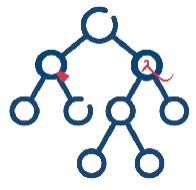
\includegraphics[height=1.0cm]{msca_logo.png}}%
    \end{center}

    \vspace{0.6cm}

    % Main title with Q logos on sides (with clickable links)
    \begin{center}
        \begin{minipage}{0.1\textwidth}
            \centering
            \href{https://quantlet.com}{
\includegraphics[height=1.1cm]{ql_logo.png}}
        \end{minipage}%
        \begin{minipage}{0.78\textwidth}
            \centering
            {\LARGE\bfseries\usebeamercolor[fg]{title}\inserttitle}

            \vspace{0.3cm}

            {\usebeamerfont{subtitle}\usebeamercolor[fg]{title}\insertsubtitle}
        \end{minipage}%
        \begin{minipage}{0.1\textwidth}
            \centering
            \href{https://quantinar.com}{
\includegraphics[height=1.1cm]{qr_logo.png}}
        \end{minipage}
    \end{center}

    \vspace{0.6cm}

    % Authors (left aligned)
    \hspace{0.5cm}{\usebeamerfont{author}\insertauthor}

    \vspace{0.3cm}

    % Institute/Affiliations (left aligned)
    \hspace{0.5cm}\begin{minipage}[t]{0.9\textwidth}
        \raggedright\small\insertinstitute
    \end{minipage}
}

%=============================================================================
% THEOREM ENVIRONMENTS
%=============================================================================
\theoremstyle{definition}
\setbeamertemplate{theorems}[numbered]
\ifdefined\atslang
\newtheorem{defn}{Definiție}
\newtheorem{thm}{Teoremă}
\newtheorem{prop}{Propoziție}
\newtheorem{rmk}{Observație}
\else
\newtheorem{defn}{Definition}
\newtheorem{thm}{Theorem}
\newtheorem{prop}{Proposition}
\newtheorem{rmk}{Remark}
\fi

%=============================================================================
% CENTRED MINIPAGE (no extra vertical space)
%=============================================================================
\newenvironment{cminipage}[1]{%
    \par\noindent\hfill\begin{minipage}{#1}\ignorespaces
}{%
    \end{minipage}\hfill\null\par
}

%=============================================================================
% CUSTOM COMMANDS
%=============================================================================
\newcommand{\E}{\mathbb{E}}
\newcommand{\Var}{\text{Var}}
\newcommand{\Cov}{\text{Cov}}
\newcommand{\Corr}{\text{Corr}}
\newcommand{\R}{\mathbb{R}}
\newcommand{\N}{\mathbb{N}}
\newcommand{\Z}{\mathbb{Z}}
\newcommand{\B}{\mathbf{B}}
\newcommand{\imark}{\textcolor{MainBlue}{\textbullet}}
\newcommand{\RMSE}{\text{RMSE}}
\newcommand{\MAE}{\text{MAE}}
\newcommand{\MAPE}{\text{MAPE}}

% Boldface vector/matrix commands (VAR, VECM, state space)
\newcommand{\bY}{\mathbf{Y}}
\newcommand{\bX}{\mathbf{X}}
\newcommand{\bA}{\mathbf{A}}
\newcommand{\bB}{\mathbf{B}}
\newcommand{\bepsilon}{\boldsymbol{\varepsilon}}
\newcommand{\bSigma}{\boldsymbol{\Sigma}}
\newcommand{\bPhi}{\boldsymbol{\Phi}}
\newcommand{\bGamma}{\boldsymbol{\Gamma}}
\newcommand{\bPi}{\boldsymbol{\Pi}}
\newcommand{\bc}{\mathbf{c}}
\newcommand{\balpha}{\boldsymbol{\alpha}}
\newcommand{\bbeta}{\boldsymbol{\beta}}
\newcommand{\bvarepsilon}{\boldsymbol{\varepsilon}}

% Seminar marks
\newcommand{\correct}{\textcolor{Forest}{\checkmark}}
\newcommand{\incorrect}{\textcolor{Crimson}{\texttimes}}
 se definește
%   \newcommand{\coursename}{Advanced Time Series Analysis and Forecasting}          (EN)
%   \newcommand{\coursename}{Analiza avansată a seriilor de timp și previziune}       (RO)  și  \def\atslang{ro}
% Fișierele .tex se află în EN/Courses, EN/Seminars, RO/Cursuri, RO/Seminarii (două niveluri sub rădăcină).
% Deck-urile sînt generate de latex/build_chapterN.py / build_seminarN.py (vezi latex/ats_build.py).

\documentclass[9pt, aspectratio=169, t]{beamer}
\providecommand{\coursename}{Advanced Time Series Analysis and Forecasting}

% Ensure content fits on slides
\setbeamersize{text margin left=8mm, text margin right=8mm}
% Smaller institute font (title page)
\setbeamerfont{institute}{size=\footnotesize}

%=============================================================================
% THEME AND STYLE CONFIGURATION
%=============================================================================
\usetheme{default}
% Using default theme for clean header/footer control

% Color Palette (matching Redispatch PDF)
\definecolor{MainBlue}{RGB}{26, 58, 110}
\definecolor{AccentBlue}{RGB}{26, 58, 110}
\definecolor{IDAred}{RGB}{205, 0, 0}
\definecolor{DarkGray}{RGB}{51, 51, 51}
\definecolor{MediumGray}{RGB}{128, 128, 128}
\definecolor{LightGray}{RGB}{248, 248, 248}
\definecolor{VeryLightGray}{RGB}{235, 235, 235}
\definecolor{KeynoteGray}{RGB}{218, 218, 218}
\definecolor{SectionGray}{RGB}{120, 120, 120}
\definecolor{FooterGray}{RGB}{100, 100, 100}
\definecolor{Crimson}{RGB}{220, 53, 69}
\definecolor{Forest}{RGB}{46, 125, 50}
\definecolor{Amber}{RGB}{181, 133, 63}
\definecolor{Orange}{RGB}{230, 126, 34}
\definecolor{Purple}{RGB}{142, 68, 173}

% Gradient background (exact Keynote 315° gradient: white to RGB 218,218,218)
\setbeamertemplate{background}{%
    \begin{tikzpicture}[remember picture, overlay]
        \shade[shading=axis, shading angle=315,
        top color=white, bottom color=KeynoteGray]
        (current page.south west) rectangle (current page.north east);
    \end{tikzpicture}%
}
% Fallback solid color for compatibility
\setbeamercolor{background canvas}{bg=}

\setbeamercolor{palette primary}{bg=MainBlue, fg=white}
\setbeamercolor{palette secondary}{bg=MainBlue!85, fg=white}
\setbeamercolor{palette tertiary}{bg=MainBlue!70, fg=white}
\setbeamercolor{structure}{fg=MainBlue}
\setbeamercolor{title}{fg=IDAred}
\setbeamercolor{frametitle}{fg=IDAred, bg=}
\setbeamercolor{block title}{bg=MainBlue, fg=white}
\setbeamercolor{block body}{bg=VeryLightGray, fg=DarkGray}
\setbeamercolor{block title alerted}{bg=Crimson, fg=white}
\setbeamercolor{block body alerted}{bg=Crimson!8, fg=DarkGray}
\setbeamercolor{block title example}{bg=Forest, fg=white}
\setbeamercolor{block body example}{bg=Forest!8, fg=DarkGray}
\setbeamercolor{item}{fg=MainBlue}

% Footer colors (override Madrid theme blue)
\setbeamercolor{author in head/foot}{fg=FooterGray, bg=}
\setbeamercolor{title in head/foot}{fg=FooterGray, bg=}
\setbeamercolor{date in head/foot}{fg=FooterGray, bg=}
\setbeamercolor{section in head/foot}{fg=FooterGray, bg=}
\setbeamercolor{subsection in head/foot}{fg=FooterGray, bg=}

% Bullet styles (apply everywhere including blocks)
\setbeamertemplate{itemize item}{\color{MainBlue}$\boxdot$}
\setbeamertemplate{itemize subitem}{\color{MainBlue}$\blacktriangleright$}
\setbeamertemplate{itemize subsubitem}{\color{MainBlue}\tiny$\bullet$}
\setbeamertemplate{itemize/enumerate body begin}{\normalsize}
\setbeamertemplate{itemize/enumerate subbody begin}{\normalsize}

% Item spacing - compact style
\setlength{\leftmargini}{10pt}       % Level 1: minimal indent
\setlength{\leftmarginii}{10pt}      % Level 2: minimal additional indent
% Compact list spacing (zero extra space before/after lists in blocks)
\makeatletter
\def\@listi{\leftmargin\leftmargini \topsep 0pt \parsep 0pt \itemsep 0pt}
\def\@listii{\leftmargin\leftmarginii \topsep 0pt \parsep 0pt \itemsep 0pt}
\makeatother

\setbeamertemplate{navigation symbols}{}

%=============================================================================
% CUSTOM HEADLINE
%=============================================================================
\setbeamertemplate{headline}{%
    \vskip10pt%
    \hbox to \paperwidth{%
        \hskip0.5cm%
        {\small\color{FooterGray}\renewcommand{\hyperlink}[2]{##2}\insertsectionhead}%
        \hfill%
        \textcolor{FooterGray}{\small\insertframenumber}%
        \hskip0.5cm%
    }%
    \vskip4pt%
    {\color{FooterGray}\hrule height 0.4pt}%
}

%=============================================================================
% CUSTOM FOOTER
%=============================================================================
\usepackage{fontawesome5}

\setbeamertemplate{footline}{%
    {\color{FooterGray}\hrule height 0.4pt}%
    \vskip4pt%
    \hbox to \paperwidth{%
        \hskip0.5cm%
        \textcolor{FooterGray}{\small\coursename}%
        \hfill%
        \raisebox{-0.1em}{%
            \begin{tikzpicture}[x=0.08em, y=0.08em, line width=0.4pt]
                \draw[FooterGray] (0,3) -- (1,4) -- (2,3.5) -- (3,5) -- (4,4) -- (5,6) -- (6,5.5) -- (7,4) -- (8,5) -- (9,7) -- (10,6) -- (11,5) -- (12,6.5) -- (13,8) -- (14,7) -- (15,6) -- (16,7.5) -- (17,9) -- (18,8) -- (19,7) -- (20,8.5) -- (21,10) -- (22,9) -- (23,8) -- (24,9.5);
            \end{tikzpicture}%
        }%
        \hskip0.5cm%
    }%
    \vskip6pt%
}

%=============================================================================
% PACKAGES
%=============================================================================
\usepackage[utf8]{inputenc}
\DeclareUnicodeCharacter{03B1}{\ensuremath{\alpha}}
\usepackage[T1]{fontenc}
\usepackage{amsmath, amssymb, amsthm}
\usepackage{mathtools}
\usepackage{bm}
\usepackage{tikz}
\usetikzlibrary{arrows.meta, positioning, shapes, calc, decorations.pathreplacing, shadings}
\usepackage{booktabs}
\usepackage{multirow}
\usepackage{array}
\usepackage{graphicx}
\usepackage{animate}
\usepackage{hyperref}
\usepackage{colortbl}
\usepackage{listings}
\lstset{language=Python, basicstyle=\ttfamily\scriptsize, keywordstyle=\color{MainBlue}\bfseries,
  commentstyle=\color{Forest}, stringstyle=\color{Crimson}, breaklines=true,
  frame=none, backgroundcolor=\color{VeryLightGray}, xleftmargin=2mm}
\hypersetup{colorlinks=true, linkcolor=MainBlue, urlcolor=MainBlue}
\graphicspath{{../../logos/}{../../charts/}{../../photos/}}
\usepackage{xcolor}
\hfuzz=2pt  % Suppress tiny overfull warnings (<2pt)
\vfuzz=2pt  % Suppress tiny vertical overfull warnings (<2pt)

%=============================================================================
% QUANTLET COMMANDS
%   \quantlet{<displayed name>}{<url>}       (generic)
%   \atsquantlet{Ch_05}{ATS_ch5_garch}       -> https://github.com/danpele/Advanced-Time-Series/tree/main/Quantlets/Ch_05/ATS_ch5_garch
%   \qlurl{<folder>} is defined per chapter by the generator (Quantlets/Ch_NN/<folder>)
%=============================================================================
\newcommand{\atsrepo}{https://github.com/danpele/Advanced-Time-Series}
\newcommand{\atsqlbase}{https://github.com/danpele/Advanced-Time-Series/tree/main/Quantlets}
\newcommand{\quantlet}[2]{%
    \hfill\href{#2}{%
        \raisebox{-0.15em}{
\includegraphics[height=0.7em]{ql_logo.png}}%
        \textcolor{MainBlue}{\tiny\ #1}%
    }%
}
\newcommand{\atsquantlet}[2]{\quantlet{\detokenize{#2}}{\atsqlbase/#1/#2}}

%=============================================================================
% NOTEBOOKS (Google Colab)
%   \colaburl{notebooks/EN/chapter5_seminar_notebook.ipynb} -> the Colab link of a file in the ATS repo
%   \nb: the chapter notebook (each seminar deck redefines it with \renewcommand)
%=============================================================================
\newcommand{\colaburl}[1]{https://colab.research.google.com/github/danpele/Advanced-Time-Series/blob/main/#1}
\newcommand{\nb}{https://colab.research.google.com/github/danpele/Advanced-Time-Series/tree/main/notebooks/EN}
\newcommand{\nbname}{notebooks/EN}

%=============================================================================
% SLIDE HELPERS (used by the generators; the same as in MFM)
%=============================================================================
% local font size for list bodies (the preamble forces \normalsize)
\newcommand{\itemsize}[1]{\setbeamertemplate{itemize/enumerate body begin}{#1}\setbeamertemplate{itemize/enumerate subbody begin}{#1}}
\newcommand{\intitle}[1]{{\hypersetup{urlcolor=white}#1}}   % white links inside coloured title bars
\newcommand{\imgcap}[1]{{\scriptsize #1}\\[0.5mm]}          % caption under a photo
\newcommand{\imgcredit}[2]{{\tiny\color{FooterGray}\href{#1}{#2}}}   % image credit: source URL, author/licence
\newcommand{\aiprompt}[1]{{\ttfamily\color{MainBlue}#1}}     % a prompt to an AI assistant

%=============================================================================
% SEMINARS: student version by default; the instructor wrapper *_solutions.tex sets \solutionstrue
%=============================================================================
\makeatletter\@ifundefined{ifsolutions}{\expandafter\newif\csname ifsolutions\endcsname}{}\makeatother
\newcommand{\solonly}[1]{\ifsolutions #1\fi}
\newcommand{\propsub}{\ifsolutions\else\framesubtitle{\ifdefined\atslang Rezolvarea se discută la seminar\else Solution discussed in class\fi}\fi}

%=============================================================================
% APPENDIX AND CHAPTER LINKS (latex/appendix_links.py writes the calls; it also re-declares these
% macros before \begin{document}, so the decks compile with or without this preamble block)
%=============================================================================
\providecommand{\atsapplink}[3]{\hypertarget{#2}{}\hyperlink{#1}{\beamergotobutton{#3}}}
\providecommand{\atsappback}[2]{\begin{tikzpicture}[remember picture,overlay]\node[anchor=south east] at ([xshift=-3mm,yshift=7mm]current page.south east){\hyperlink{#1}{\beamerreturnbutton{#2}}};\end{tikzpicture}}
\providecommand{\atschlink}[2]{\href{#1}{#2}}
\providecommand{\atschlinkt}[2]{\href{#1}{\usebeamercolor[fg]{frametitle}#2}}

%=============================================================================
% QUANTINAR COMMAND: link către un curs Quantinar (subiecte avansate)
%=============================================================================
\newcommand{\quantinar}[2]{%
    \href{#2}{%
        \raisebox{-0.15em}{
\includegraphics[height=0.8em]{qr_logo.png}}%
        \textcolor{MainBlue}{\scriptsize\ #1}%
    }%
}

%=============================================================================
% CUSTOM TITLE PAGE
%=============================================================================
\defbeamertemplate*{title page}{hybrid}[1][]
{
    \vspace{0.2cm}
    % Logos row - top header (with clickable links)
    \begin{center}
        \href{https://www.ase.ro}{
\includegraphics[height=1.0cm]{ase_logo.png}}\hspace{0.3cm}%
        \href{https://theida.net}{
\includegraphics[height=1.0cm]{ida_logo.png}}\hspace{0.3cm}%
        \href{https://blockchain-research-center.com}{
\includegraphics[height=1.0cm]{brc_logo.png}}\hspace{0.3cm}%
        \href{https://www.ai4efin.ase.ro}{
\includegraphics[height=1.0cm]{ai4efin_logo.png}}\hspace{0.3cm}%
        \href{https://ipe.ro/new}{
\includegraphics[height=1.0cm]{acad_logo.png}}\hspace{0.3cm}%
        \href{https://www.digital-finance-msca.com}{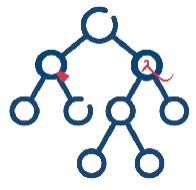
\includegraphics[height=1.0cm]{msca_logo.png}}%
    \end{center}

    \vspace{0.6cm}

    % Main title with Q logos on sides (with clickable links)
    \begin{center}
        \begin{minipage}{0.1\textwidth}
            \centering
            \href{https://quantlet.com}{
\includegraphics[height=1.1cm]{ql_logo.png}}
        \end{minipage}%
        \begin{minipage}{0.78\textwidth}
            \centering
            {\LARGE\bfseries\usebeamercolor[fg]{title}\inserttitle}

            \vspace{0.3cm}

            {\usebeamerfont{subtitle}\usebeamercolor[fg]{title}\insertsubtitle}
        \end{minipage}%
        \begin{minipage}{0.1\textwidth}
            \centering
            \href{https://quantinar.com}{
\includegraphics[height=1.1cm]{qr_logo.png}}
        \end{minipage}
    \end{center}

    \vspace{0.6cm}

    % Authors (left aligned)
    \hspace{0.5cm}{\usebeamerfont{author}\insertauthor}

    \vspace{0.3cm}

    % Institute/Affiliations (left aligned)
    \hspace{0.5cm}\begin{minipage}[t]{0.9\textwidth}
        \raggedright\small\insertinstitute
    \end{minipage}
}

%=============================================================================
% THEOREM ENVIRONMENTS
%=============================================================================
\theoremstyle{definition}
\setbeamertemplate{theorems}[numbered]
\ifdefined\atslang
\newtheorem{defn}{Definiție}
\newtheorem{thm}{Teoremă}
\newtheorem{prop}{Propoziție}
\newtheorem{rmk}{Observație}
\else
\newtheorem{defn}{Definition}
\newtheorem{thm}{Theorem}
\newtheorem{prop}{Proposition}
\newtheorem{rmk}{Remark}
\fi

%=============================================================================
% CENTRED MINIPAGE (no extra vertical space)
%=============================================================================
\newenvironment{cminipage}[1]{%
    \par\noindent\hfill\begin{minipage}{#1}\ignorespaces
}{%
    \end{minipage}\hfill\null\par
}

%=============================================================================
% CUSTOM COMMANDS
%=============================================================================
\newcommand{\E}{\mathbb{E}}
\newcommand{\Var}{\text{Var}}
\newcommand{\Cov}{\text{Cov}}
\newcommand{\Corr}{\text{Corr}}
\newcommand{\R}{\mathbb{R}}
\newcommand{\N}{\mathbb{N}}
\newcommand{\Z}{\mathbb{Z}}
\newcommand{\B}{\mathbf{B}}
\newcommand{\imark}{\textcolor{MainBlue}{\textbullet}}
\newcommand{\RMSE}{\text{RMSE}}
\newcommand{\MAE}{\text{MAE}}
\newcommand{\MAPE}{\text{MAPE}}

% Boldface vector/matrix commands (VAR, VECM, state space)
\newcommand{\bY}{\mathbf{Y}}
\newcommand{\bX}{\mathbf{X}}
\newcommand{\bA}{\mathbf{A}}
\newcommand{\bB}{\mathbf{B}}
\newcommand{\bepsilon}{\boldsymbol{\varepsilon}}
\newcommand{\bSigma}{\boldsymbol{\Sigma}}
\newcommand{\bPhi}{\boldsymbol{\Phi}}
\newcommand{\bGamma}{\boldsymbol{\Gamma}}
\newcommand{\bPi}{\boldsymbol{\Pi}}
\newcommand{\bc}{\mathbf{c}}
\newcommand{\balpha}{\boldsymbol{\alpha}}
\newcommand{\bbeta}{\boldsymbol{\beta}}
\newcommand{\bvarepsilon}{\boldsymbol{\varepsilon}}

% Seminar marks
\newcommand{\correct}{\textcolor{Forest}{\checkmark}}
\newcommand{\incorrect}{\textcolor{Crimson}{\texttimes}}
 se definește
%   \newcommand{\coursename}{Advanced Time Series Analysis and Forecasting}          (EN)
%   \newcommand{\coursename}{Analiza avansată a seriilor de timp și previziune}       (RO)  și  \def\atslang{ro}
% Fișierele .tex se află în EN/Courses, EN/Seminars, RO/Cursuri, RO/Seminarii (două niveluri sub rădăcină).
% Deck-urile sînt generate de latex/build_chapterN.py / build_seminarN.py (vezi latex/ats_build.py).

\documentclass[9pt, aspectratio=169, t]{beamer}
\providecommand{\coursename}{Advanced Time Series Analysis and Forecasting}

% Ensure content fits on slides
\setbeamersize{text margin left=8mm, text margin right=8mm}
% Smaller institute font (title page)
\setbeamerfont{institute}{size=\footnotesize}

%=============================================================================
% THEME AND STYLE CONFIGURATION
%=============================================================================
\usetheme{default}
% Using default theme for clean header/footer control

% Color Palette (matching Redispatch PDF)
\definecolor{MainBlue}{RGB}{26, 58, 110}
\definecolor{AccentBlue}{RGB}{26, 58, 110}
\definecolor{IDAred}{RGB}{205, 0, 0}
\definecolor{DarkGray}{RGB}{51, 51, 51}
\definecolor{MediumGray}{RGB}{128, 128, 128}
\definecolor{LightGray}{RGB}{248, 248, 248}
\definecolor{VeryLightGray}{RGB}{235, 235, 235}
\definecolor{KeynoteGray}{RGB}{218, 218, 218}
\definecolor{SectionGray}{RGB}{120, 120, 120}
\definecolor{FooterGray}{RGB}{100, 100, 100}
\definecolor{Crimson}{RGB}{220, 53, 69}
\definecolor{Forest}{RGB}{46, 125, 50}
\definecolor{Amber}{RGB}{181, 133, 63}
\definecolor{Orange}{RGB}{230, 126, 34}
\definecolor{Purple}{RGB}{142, 68, 173}

% Gradient background (exact Keynote 315° gradient: white to RGB 218,218,218)
\setbeamertemplate{background}{%
    \begin{tikzpicture}[remember picture, overlay]
        \shade[shading=axis, shading angle=315,
        top color=white, bottom color=KeynoteGray]
        (current page.south west) rectangle (current page.north east);
    \end{tikzpicture}%
}
% Fallback solid color for compatibility
\setbeamercolor{background canvas}{bg=}

\setbeamercolor{palette primary}{bg=MainBlue, fg=white}
\setbeamercolor{palette secondary}{bg=MainBlue!85, fg=white}
\setbeamercolor{palette tertiary}{bg=MainBlue!70, fg=white}
\setbeamercolor{structure}{fg=MainBlue}
\setbeamercolor{title}{fg=IDAred}
\setbeamercolor{frametitle}{fg=IDAred, bg=}
\setbeamercolor{block title}{bg=MainBlue, fg=white}
\setbeamercolor{block body}{bg=VeryLightGray, fg=DarkGray}
\setbeamercolor{block title alerted}{bg=Crimson, fg=white}
\setbeamercolor{block body alerted}{bg=Crimson!8, fg=DarkGray}
\setbeamercolor{block title example}{bg=Forest, fg=white}
\setbeamercolor{block body example}{bg=Forest!8, fg=DarkGray}
\setbeamercolor{item}{fg=MainBlue}

% Footer colors (override Madrid theme blue)
\setbeamercolor{author in head/foot}{fg=FooterGray, bg=}
\setbeamercolor{title in head/foot}{fg=FooterGray, bg=}
\setbeamercolor{date in head/foot}{fg=FooterGray, bg=}
\setbeamercolor{section in head/foot}{fg=FooterGray, bg=}
\setbeamercolor{subsection in head/foot}{fg=FooterGray, bg=}

% Bullet styles (apply everywhere including blocks)
\setbeamertemplate{itemize item}{\color{MainBlue}$\boxdot$}
\setbeamertemplate{itemize subitem}{\color{MainBlue}$\blacktriangleright$}
\setbeamertemplate{itemize subsubitem}{\color{MainBlue}\tiny$\bullet$}
\setbeamertemplate{itemize/enumerate body begin}{\normalsize}
\setbeamertemplate{itemize/enumerate subbody begin}{\normalsize}

% Item spacing - compact style
\setlength{\leftmargini}{10pt}       % Level 1: minimal indent
\setlength{\leftmarginii}{10pt}      % Level 2: minimal additional indent
% Compact list spacing (zero extra space before/after lists in blocks)
\makeatletter
\def\@listi{\leftmargin\leftmargini \topsep 0pt \parsep 0pt \itemsep 0pt}
\def\@listii{\leftmargin\leftmarginii \topsep 0pt \parsep 0pt \itemsep 0pt}
\makeatother

\setbeamertemplate{navigation symbols}{}

%=============================================================================
% CUSTOM HEADLINE
%=============================================================================
\setbeamertemplate{headline}{%
    \vskip10pt%
    \hbox to \paperwidth{%
        \hskip0.5cm%
        {\small\color{FooterGray}\renewcommand{\hyperlink}[2]{##2}\insertsectionhead}%
        \hfill%
        \textcolor{FooterGray}{\small\insertframenumber}%
        \hskip0.5cm%
    }%
    \vskip4pt%
    {\color{FooterGray}\hrule height 0.4pt}%
}

%=============================================================================
% CUSTOM FOOTER
%=============================================================================
\usepackage{fontawesome5}

\setbeamertemplate{footline}{%
    {\color{FooterGray}\hrule height 0.4pt}%
    \vskip4pt%
    \hbox to \paperwidth{%
        \hskip0.5cm%
        \textcolor{FooterGray}{\small\coursename}%
        \hfill%
        \raisebox{-0.1em}{%
            \begin{tikzpicture}[x=0.08em, y=0.08em, line width=0.4pt]
                \draw[FooterGray] (0,3) -- (1,4) -- (2,3.5) -- (3,5) -- (4,4) -- (5,6) -- (6,5.5) -- (7,4) -- (8,5) -- (9,7) -- (10,6) -- (11,5) -- (12,6.5) -- (13,8) -- (14,7) -- (15,6) -- (16,7.5) -- (17,9) -- (18,8) -- (19,7) -- (20,8.5) -- (21,10) -- (22,9) -- (23,8) -- (24,9.5);
            \end{tikzpicture}%
        }%
        \hskip0.5cm%
    }%
    \vskip6pt%
}

%=============================================================================
% PACKAGES
%=============================================================================
\usepackage[utf8]{inputenc}
\DeclareUnicodeCharacter{03B1}{\ensuremath{\alpha}}
\usepackage[T1]{fontenc}
\usepackage{amsmath, amssymb, amsthm}
\usepackage{mathtools}
\usepackage{bm}
\usepackage{tikz}
\usetikzlibrary{arrows.meta, positioning, shapes, calc, decorations.pathreplacing, shadings}
\usepackage{booktabs}
\usepackage{multirow}
\usepackage{array}
\usepackage{graphicx}
\usepackage{animate}
\usepackage{hyperref}
\usepackage{colortbl}
\usepackage{listings}
\lstset{language=Python, basicstyle=\ttfamily\scriptsize, keywordstyle=\color{MainBlue}\bfseries,
  commentstyle=\color{Forest}, stringstyle=\color{Crimson}, breaklines=true,
  frame=none, backgroundcolor=\color{VeryLightGray}, xleftmargin=2mm}
\hypersetup{colorlinks=true, linkcolor=MainBlue, urlcolor=MainBlue}
\graphicspath{{../../logos/}{../../charts/}{../../photos/}}
\usepackage{xcolor}
\hfuzz=2pt  % Suppress tiny overfull warnings (<2pt)
\vfuzz=2pt  % Suppress tiny vertical overfull warnings (<2pt)

%=============================================================================
% QUANTLET COMMANDS
%   \quantlet{<displayed name>}{<url>}       (generic)
%   \atsquantlet{Ch_05}{ATS_ch5_garch}       -> https://github.com/danpele/Advanced-Time-Series/tree/main/Quantlets/Ch_05/ATS_ch5_garch
%   \qlurl{<folder>} is defined per chapter by the generator (Quantlets/Ch_NN/<folder>)
%=============================================================================
\newcommand{\atsrepo}{https://github.com/danpele/Advanced-Time-Series}
\newcommand{\atsqlbase}{https://github.com/danpele/Advanced-Time-Series/tree/main/Quantlets}
\newcommand{\quantlet}[2]{%
    \hfill\href{#2}{%
        \raisebox{-0.15em}{
\includegraphics[height=0.7em]{ql_logo.png}}%
        \textcolor{MainBlue}{\tiny\ #1}%
    }%
}
\newcommand{\atsquantlet}[2]{\quantlet{\detokenize{#2}}{\atsqlbase/#1/#2}}

%=============================================================================
% NOTEBOOKS (Google Colab)
%   \colaburl{notebooks/EN/chapter5_seminar_notebook.ipynb} -> the Colab link of a file in the ATS repo
%   \nb: the chapter notebook (each seminar deck redefines it with \renewcommand)
%=============================================================================
\newcommand{\colaburl}[1]{https://colab.research.google.com/github/danpele/Advanced-Time-Series/blob/main/#1}
\newcommand{\nb}{https://colab.research.google.com/github/danpele/Advanced-Time-Series/tree/main/notebooks/EN}
\newcommand{\nbname}{notebooks/EN}

%=============================================================================
% SLIDE HELPERS (used by the generators; the same as in MFM)
%=============================================================================
% local font size for list bodies (the preamble forces \normalsize)
\newcommand{\itemsize}[1]{\setbeamertemplate{itemize/enumerate body begin}{#1}\setbeamertemplate{itemize/enumerate subbody begin}{#1}}
\newcommand{\intitle}[1]{{\hypersetup{urlcolor=white}#1}}   % white links inside coloured title bars
\newcommand{\imgcap}[1]{{\scriptsize #1}\\[0.5mm]}          % caption under a photo
\newcommand{\imgcredit}[2]{{\tiny\color{FooterGray}\href{#1}{#2}}}   % image credit: source URL, author/licence
\newcommand{\aiprompt}[1]{{\ttfamily\color{MainBlue}#1}}     % a prompt to an AI assistant

%=============================================================================
% SEMINARS: student version by default; the instructor wrapper *_solutions.tex sets \solutionstrue
%=============================================================================
\makeatletter\@ifundefined{ifsolutions}{\expandafter\newif\csname ifsolutions\endcsname}{}\makeatother
\newcommand{\solonly}[1]{\ifsolutions #1\fi}
\newcommand{\propsub}{\ifsolutions\else\framesubtitle{\ifdefined\atslang Rezolvarea se discută la seminar\else Solution discussed in class\fi}\fi}

%=============================================================================
% APPENDIX AND CHAPTER LINKS (latex/appendix_links.py writes the calls; it also re-declares these
% macros before \begin{document}, so the decks compile with or without this preamble block)
%=============================================================================
\providecommand{\atsapplink}[3]{\hypertarget{#2}{}\hyperlink{#1}{\beamergotobutton{#3}}}
\providecommand{\atsappback}[2]{\begin{tikzpicture}[remember picture,overlay]\node[anchor=south east] at ([xshift=-3mm,yshift=7mm]current page.south east){\hyperlink{#1}{\beamerreturnbutton{#2}}};\end{tikzpicture}}
\providecommand{\atschlink}[2]{\href{#1}{#2}}
\providecommand{\atschlinkt}[2]{\href{#1}{\usebeamercolor[fg]{frametitle}#2}}

%=============================================================================
% QUANTINAR COMMAND: link către un curs Quantinar (subiecte avansate)
%=============================================================================
\newcommand{\quantinar}[2]{%
    \href{#2}{%
        \raisebox{-0.15em}{
\includegraphics[height=0.8em]{qr_logo.png}}%
        \textcolor{MainBlue}{\scriptsize\ #1}%
    }%
}

%=============================================================================
% CUSTOM TITLE PAGE
%=============================================================================
\defbeamertemplate*{title page}{hybrid}[1][]
{
    \vspace{0.2cm}
    % Logos row - top header (with clickable links)
    \begin{center}
        \href{https://www.ase.ro}{
\includegraphics[height=1.0cm]{ase_logo.png}}\hspace{0.3cm}%
        \href{https://theida.net}{
\includegraphics[height=1.0cm]{ida_logo.png}}\hspace{0.3cm}%
        \href{https://blockchain-research-center.com}{
\includegraphics[height=1.0cm]{brc_logo.png}}\hspace{0.3cm}%
        \href{https://www.ai4efin.ase.ro}{
\includegraphics[height=1.0cm]{ai4efin_logo.png}}\hspace{0.3cm}%
        \href{https://ipe.ro/new}{
\includegraphics[height=1.0cm]{acad_logo.png}}\hspace{0.3cm}%
        \href{https://www.digital-finance-msca.com}{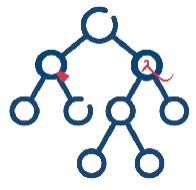
\includegraphics[height=1.0cm]{msca_logo.png}}%
    \end{center}

    \vspace{0.6cm}

    % Main title with Q logos on sides (with clickable links)
    \begin{center}
        \begin{minipage}{0.1\textwidth}
            \centering
            \href{https://quantlet.com}{
\includegraphics[height=1.1cm]{ql_logo.png}}
        \end{minipage}%
        \begin{minipage}{0.78\textwidth}
            \centering
            {\LARGE\bfseries\usebeamercolor[fg]{title}\inserttitle}

            \vspace{0.3cm}

            {\usebeamerfont{subtitle}\usebeamercolor[fg]{title}\insertsubtitle}
        \end{minipage}%
        \begin{minipage}{0.1\textwidth}
            \centering
            \href{https://quantinar.com}{
\includegraphics[height=1.1cm]{qr_logo.png}}
        \end{minipage}
    \end{center}

    \vspace{0.6cm}

    % Authors (left aligned)
    \hspace{0.5cm}{\usebeamerfont{author}\insertauthor}

    \vspace{0.3cm}

    % Institute/Affiliations (left aligned)
    \hspace{0.5cm}\begin{minipage}[t]{0.9\textwidth}
        \raggedright\small\insertinstitute
    \end{minipage}
}

%=============================================================================
% THEOREM ENVIRONMENTS
%=============================================================================
\theoremstyle{definition}
\setbeamertemplate{theorems}[numbered]
\ifdefined\atslang
\newtheorem{defn}{Definiție}
\newtheorem{thm}{Teoremă}
\newtheorem{prop}{Propoziție}
\newtheorem{rmk}{Observație}
\else
\newtheorem{defn}{Definition}
\newtheorem{thm}{Theorem}
\newtheorem{prop}{Proposition}
\newtheorem{rmk}{Remark}
\fi

%=============================================================================
% CENTRED MINIPAGE (no extra vertical space)
%=============================================================================
\newenvironment{cminipage}[1]{%
    \par\noindent\hfill\begin{minipage}{#1}\ignorespaces
}{%
    \end{minipage}\hfill\null\par
}

%=============================================================================
% CUSTOM COMMANDS
%=============================================================================
\newcommand{\E}{\mathbb{E}}
\newcommand{\Var}{\text{Var}}
\newcommand{\Cov}{\text{Cov}}
\newcommand{\Corr}{\text{Corr}}
\newcommand{\R}{\mathbb{R}}
\newcommand{\N}{\mathbb{N}}
\newcommand{\Z}{\mathbb{Z}}
\newcommand{\B}{\mathbf{B}}
\newcommand{\imark}{\textcolor{MainBlue}{\textbullet}}
\newcommand{\RMSE}{\text{RMSE}}
\newcommand{\MAE}{\text{MAE}}
\newcommand{\MAPE}{\text{MAPE}}

% Boldface vector/matrix commands (VAR, VECM, state space)
\newcommand{\bY}{\mathbf{Y}}
\newcommand{\bX}{\mathbf{X}}
\newcommand{\bA}{\mathbf{A}}
\newcommand{\bB}{\mathbf{B}}
\newcommand{\bepsilon}{\boldsymbol{\varepsilon}}
\newcommand{\bSigma}{\boldsymbol{\Sigma}}
\newcommand{\bPhi}{\boldsymbol{\Phi}}
\newcommand{\bGamma}{\boldsymbol{\Gamma}}
\newcommand{\bPi}{\boldsymbol{\Pi}}
\newcommand{\bc}{\mathbf{c}}
\newcommand{\balpha}{\boldsymbol{\alpha}}
\newcommand{\bbeta}{\boldsymbol{\beta}}
\newcommand{\bvarepsilon}{\boldsymbol{\varepsilon}}

% Seminar marks
\newcommand{\correct}{\textcolor{Forest}{\checkmark}}
\newcommand{\incorrect}{\textcolor{Crimson}{\texttimes}}


\newcommand{\qlurl}[1]{https://github.com/danpele/Advanced-Time-Series/tree/main/Quantlets/Ch_12/#1}

% Clickable citations (DOIs verified via Crossref)
\newcommand{\refBaiK}{\href{https://arxiv.org/abs/1803.01271}{Bai, Kolter și Koltun (2018)}}
\newcommand{\refBCH}{\href{https://doi.org/10.1093/restud/rdt044}{Belloni, Chernozhukov și Hansen (2014)}}
\newcommand{\refBSF}{\href{https://doi.org/10.1109/72.279181}{Bengio, Simard și Frasconi (1994)}}
\newcommand{\refBen}{\href{https://doi.org/10.1145/3533382}{Benidis et al.\ (2022)}}
\newcommand{\refBB}{\href{https://doi.org/10.1016/j.ins.2011.12.028}{Bergmeir și Benítez (2012)}}
\newcommand{\refBHK}{\href{https://doi.org/10.1016/j.csda.2017.11.003}{Bergmeir, Hyndman și Koo (2018)}}
\newcommand{\refBerk}{\href{https://doi.org/10.1214/12-AOS1077}{Berk et al.\ (2013)}}
\newcommand{\refBM}{\href{https://doi.org/10.1214/15-AOS1315}{Basu și Michailidis (2015)}}
\newcommand{\refBreA}{\href{https://doi.org/10.1007/BF00058655}{Breiman (1996)}}
\newcommand{\refBreB}{\href{https://doi.org/10.1023/A:1010933404324}{Breiman (2001)}}
\newcommand{\refBuc}{\href{https://doi.org/10.1093/jjfinec/nbaa008}{Bucci (2020)}}
\newcommand{\refBCN}{\href{https://doi.org/10.1093/biomet/81.2.351}{Burman, Chow și Nolan (1994)}}
\newcommand{\refNHiTS}{\href{https://doi.org/10.1609/aaai.v37i6.25854}{Challu et al.\ (2023)}}
\newcommand{\refCG}{\href{https://doi.org/10.1145/2939672.2939785}{Chen și Guestrin (2016)}}
\newcommand{\refCho}{\href{https://doi.org/10.3115/v1/D14-1179}{Cho et al.\ (2014)}}
\newcommand{\refCSV}{\href{https://doi.org/10.1093/jjfinec/nbac020}{Christensen, Siggaard și Veliyev (2023)}}
\newcommand{\refCor}{\href{https://doi.org/10.1093/jjfinec/nbp001}{Corsi (2009)}}
\newcommand{\refDM}{\href{https://doi.org/10.1080/07350015.1995.10524599}{Diebold și Mariano (1995)}}
\newcommand{\refFri}{\href{https://doi.org/10.1214/aos/1013203451}{Friedman (2001)}}
\newcommand{\refGSC}{\href{https://doi.org/10.1162/089976600300015015}{Gers, Schmidhuber și Cummins (2000)}}
\newcommand{\refGR}{\href{https://doi.org/10.1198/016214506000001437}{Gneiting și Raftery (2007)}}
\newcommand{\refGCLSS}{\href{https://doi.org/10.1002/jae.2910}{Goulet Coulombe et al.\ (2022)}}
\newcommand{\refGKX}{\href{https://doi.org/10.1093/rfs/hhaa009}{Gu, Kelly și Xiu (2020)}}
\newcommand{\refHan}{\href{https://doi.org/10.1198/073500105000000063}{Hansen (2005)}}
\newcommand{\refHLN}{\href{https://doi.org/10.3982/ECTA5771}{Hansen, Lunde și Nason (2011)}}
\newcommand{\refOMI}{\href{https://web.archive.org/web/20220301022212/https://realized.oxford-man.ox.ac.uk/}{Heber et al.\ (2009)}}
\newcommand{\refHAB}{\href{https://doi.org/10.1007/s10618-022-00894-5}{Hewamalage, Ackermann și Bergmeir (2023)}}
\newcommand{\refHBB}{\href{https://doi.org/10.1016/j.ijforecast.2020.06.008}{Hewamalage, Bergmeir și Bandara (2021)}}
\newcommand{\refHS}{\href{https://doi.org/10.1162/neco.1997.9.8.1735}{Hochreiter și Schmidhuber (1997)}}
\newcommand{\refHK}{\href{https://doi.org/10.1016/j.ijforecast.2006.03.001}{Hyndman și Koehler (2006)}}
\newcommand{\refJW}{\href{https://doi.org/10.18653/v1/N19-1357}{Jain și Wallace (2019)}}
\newcommand{\refJZS}{\href{https://proceedings.mlr.press/v37/jozefowicz15.html}{Jozefowicz, Zaremba și Sutskever (2015)}}
\newcommand{\refKeA}{\href{https://proceedings.neurips.cc/paper/2017/hash/6449f44a102fde848669bdd9eb6b76fa-Abstract.html}{Ke et al.\ (2017)}}
\newcommand{\refKB}{\href{https://arxiv.org/abs/1412.6980}{Kingma și Ba (2015)}}
\newcommand{\refLMDW}{\href{https://doi.org/10.1016/j.apenergy.2021.116983}{Lago et al.\ (2021)}}
\newcommand{\refLSST}{\href{https://doi.org/10.1214/15-AOS1371}{Lee et al.\ (2016)}}
\newcommand{\refTFT}{\href{https://doi.org/10.1016/j.ijforecast.2021.03.012}{Lim et al.\ (2021)}}
\newcommand{\refLL}{\href{https://proceedings.neurips.cc/paper/2017/hash/8a20a8621978632d76c43dfd28b67767-Abstract.html}{Lundberg și Lee (2017)}}
\newcommand{\refMSAa}{\href{https://doi.org/10.1371/journal.pone.0194889}{Makridakis, Spiliotis și Assimakopoulos (2018)}}
\newcommand{\refMfourA}{\href{https://doi.org/10.1016/j.ijforecast.2019.04.014}{Makridakis, Spiliotis și Assimakopoulos (2020)}}
\newcommand{\refMfiveA}{\href{https://doi.org/10.1016/j.ijforecast.2021.11.013}{Makridakis, Spiliotis și Assimakopoulos (2022)}}
\newcommand{\refMM}{\href{https://doi.org/10.1016/j.jeconom.2015.10.011}{Medeiros și Mendes (2016)}}
\newcommand{\refMVVZ}{\href{https://doi.org/10.1080/07350015.2019.1637745}{Medeiros et al.\ (2021)}}
\newcommand{\refMei}{\href{https://jmlr.org/papers/v7/meinshausen06a.html}{Meinshausen (2006)}}
\newcommand{\refMR}{\href{https://jmlr.org/papers/v11/mohri10a.html}{Mohri și Rostamizadeh (2010)}}
\newcommand{\refMMH}{\href{https://doi.org/10.1016/j.ijforecast.2021.03.004}{Montero-Manso și Hyndman (2021)}}
\newcommand{\refNie}{\href{https://arxiv.org/abs/2211.14730}{Nie et al.\ (2023)}}
\newcommand{\refOre}{\href{https://arxiv.org/abs/1905.10437}{Oreshkin et al.\ (2020)}}
\newcommand{\refPMB}{\href{https://proceedings.mlr.press/v28/pascanu13.html}{Pascanu, Mikolov și Bengio (2013)}}
\newcommand{\refPat}{\href{https://doi.org/10.1016/j.jeconom.2010.03.034}{Patton (2011)}}
\newcommand{\refPet}{\href{https://doi.org/10.1016/j.ijforecast.2021.11.001}{Petropoulos et al.\ (2022)}}
\newcommand{\refRac}{\href{https://doi.org/10.1016/S0304-4076(00)00030-0}{Racine (2000)}}
\newcommand{\refRHW}{\href{https://doi.org/10.1038/323533a0}{Rumelhart, Hinton și Williams (1986)}}
\newcommand{\refDeepAR}{\href{https://doi.org/10.1016/j.ijforecast.2019.07.001}{Salinas et al.\ (2020)}}
\newcommand{\refSBV}{\href{https://doi.org/10.1214/15-AOS1321}{Scornet, Biau și Vert (2015)}}
\newcommand{\refSha}{\href{https://doi.org/10.1515/9781400881970-018}{Shapley (1953)}}
\newcommand{\refSmyl}{\href{https://doi.org/10.1016/j.ijforecast.2019.03.017}{Smyl (2020)}}
\newcommand{\refSVL}{\href{https://arxiv.org/abs/1409.3215}{Sutskever, Vinyals și Le (2014)}}
\newcommand{\refTib}{\href{https://doi.org/10.1111/j.2517-6161.1996.tb02080.x}{Tibshirani (1996)}}
\newcommand{\refWaveNet}{\href{https://arxiv.org/abs/1609.03499}{van den Oord et al.\ (2016)}}
\newcommand{\refVas}{\href{https://proceedings.neurips.cc/paper/2017/hash/3f5ee243547dee91fbd053c1c4a845aa-Abstract.html}{Vaswani et al.\ (2017)}}
\newcommand{\refWA}{\href{https://doi.org/10.1080/01621459.2017.1319839}{Wager și Athey (2018)}}
\newcommand{\refWhi}{\href{https://doi.org/10.1111/1468-0262.00152}{White (2000)}}
\newcommand{\refWP}{\href{https://doi.org/10.18653/v1/D19-1002}{Wiegreffe și Pinter (2019)}}
\newcommand{\refAuto}{\href{https://proceedings.neurips.cc/paper/2021/hash/bcc0d400288793e8bdcd7c19a8ac0c2b-Abstract.html}{Wu et al.\ (2021)}}
\newcommand{\refYu}{\href{https://doi.org/10.1214/aop/1176988849}{Yu (1994)}}
\newcommand{\refZeng}{\href{https://doi.org/10.1609/aaai.v37i9.26317}{Zeng et al.\ (2023)}}
\newcommand{\refZY}{\href{https://jmlr.org/papers/v7/zhao06a.html}{Zhao și Yu (2006)}}
\newcommand{\refInf}{\href{https://doi.org/10.1609/aaai.v35i12.17325}{Zhou et al.\ (2021)}}
\newcommand{\refZW}{\href{https://doi.org/10.1016/j.eneco.2017.12.016}{Ziel și Weron (2018)}}
\newcommand{\refZou}{\href{https://doi.org/10.1198/016214506000000735}{Zou (2006)}}
\newcommand{\refZH}{\href{https://doi.org/10.1111/j.1467-9868.2005.00503.x}{Zou și Hastie (2005)}}

\title[Analiza avansată a seriilor de timp și previziune]{Analiza avansată a seriilor de timp și previziune}
\subtitle{Capitolul 12: Machine learning și deep learning pentru serii de timp}
\author[D.T. Pele]{Daniel Traian PELE}
\institute{Academia de Studii Economice din București\\
IDA Institute Digital Assets\\
Blockchain Research Center\\
AI4EFin Artificial Intelligence for Energy Finance\\
Academia Română, Institutul de Prognoză Economică\\
MSCA Digital Finance}
\date{}

%=============================================================================
\providecommand{\atsapplink}[3]{\hypertarget{#2}{}\hyperlink{#1}{\beamergotobutton{#3}}}  % APPLINKS-MACROS
\providecommand{\atsappback}[2]{\begin{tikzpicture}[remember picture,overlay]\node[anchor=south east] at ([xshift=-3mm,yshift=7mm]current page.south east){\hyperlink{#1}{\beamerreturnbutton{#2}}};\end{tikzpicture}}  % APPLINKS-MACROS
\providecommand{\atschlink}[2]{\href{#1}{#2}}  % APPLINKS-MACROS
\providecommand{\atschlinkt}[2]{\href{#1}{\usebeamercolor[fg]{frametitle}#2}}  % APPLINKS-MACROS
\begin{document}
%=============================================================================

{
\setbeamertemplate{headline}{}
\setbeamertemplate{footline}{}
\begin{frame}[noframenumbering]
    \titlepage
\end{frame}
}
% BEGIN-ACRONYMS (generat de latex/acronyms.py; nu editati manual)
\begin{frame}{Acronime folosite în acest material (1/3)}
\setbeamertemplate{itemize/enumerate body begin}{\tiny}
\begin{columns}[T]
\begin{column}{0.49\textwidth}
\begin{itemize}\setlength{\itemsep}{0pt}
    \item \textbf{ACF}: Autocorrelation Function (funcția de autocorelație)
    \item \textbf{AI}: Artificial Intelligence (inteligență artificială)
    \item \textbf{AR}: AutoRegressive (model); in event studies: Abnormal Return (model autoregresiv; în studiile de eveniment: randament anormal)
    \item \textbf{ARMA}: AutoRegressive Moving Average (model) — model autoregresiv cu medie mobilă
    \item \textbf{ARX}: AutoRegressive model with eXogenous variables (model autoregresiv cu variabile exogene)
    \item \textbf{BET}: Bucharest Exchange Trading (index) — indicele de referință al Bursei de Valori București
    \item \textbf{BPTT}: BackPropagation Through Time (retropropagarea în timp)
    \item \textbf{CRPS}: Continuous Ranked Probability Score (scorul probabilistic continuu)
    \item \textbf{DM}: Diebold–Mariano (test) — testul Diebold–Mariano de comparare a prognozelor
    \item \textbf{ENTSO-E}: European Network of Transmission System Operators for Electricity (Rețeaua europeană a operatorilor de transport și de sistem pentru energie electrică)
    \item \textbf{ERM}: Empirical Risk Minimisation (minimizarea riscului empiric)
    \item \textbf{ES-RNN}: Exponential Smoothing – Recurrent Neural Network (hybrid) — hibridul netezire exponențială – rețea recurentă (Smyl 2020)
    \item \textbf{ETS}: Error, Trend, Seasonality (exponential smoothing state space models) — eroare, trend, sezonalitate (modele de netezire exponențială)
\end{itemize}
\end{column}
\begin{column}{0.49\textwidth}
\begin{itemize}\setlength{\itemsep}{0pt}
    \item \textbf{ETT}: Electricity Transformer Temperature (data set) — setul de date Electricity Transformer Temperature
    \item \textbf{FFT}: Fast Fourier Transform (transformata Fourier rapidă)
    \item \textbf{GARCH}: Generalised AutoRegressive Conditional Heteroskedasticity (heteroscedasticitate condiționată autoregresivă generalizată)
    \item \textbf{GRN}: Gated Residual Network (rețea reziduală cu poartă)
    \item \textbf{GRU}: Gated Recurrent Unit (unitate recurentă cu porți)
    \item \textbf{HAC}: Heteroskedasticity and Autocorrelation Consistent (standard errors) — erori standard robuste la heteroscedasticitate și autocorelație
    \item \textbf{HAR}: Heterogeneous AutoRegressive (model) — model autoregresiv heterogen
    \item \textbf{HGB}: Histogram Gradient Boosting (gradient boosting pe histograme)
    \item \textbf{HLN}: Harvey–Leybourne–Newbold (small-sample correction of the DM test) — corecția Harvey–Leybourne–Newbold a testului DM pentru eșantioane mici
    \item \textbf{IAPC}: Indicele armonizat al prețurilor de consum
    \item \textbf{KKT}: Karush–Kuhn–Tucker (conditions) — condițiile Karush–Kuhn–Tucker
    \item \textbf{LLM}: Large Language Model (model lingvistic de mari dimensiuni)
    \item \textbf{LOOCV}: Leave-One-Out Cross-Validation (validare încrucișată cu omiterea cîte unei observații)
\end{itemize}
\end{column}
\end{columns}
\end{frame}
\begin{frame}{Acronime folosite în acest material (2/3)}
\setbeamertemplate{itemize/enumerate body begin}{\tiny}
\begin{columns}[T]
\begin{column}{0.49\textwidth}
\begin{itemize}\setlength{\itemsep}{0pt}
    \item \textbf{LSTM}: Long Short-Term Memory (network) — rețea cu memorie pe termen lung și scurt
    \item \textbf{LTSF}: Long-Term Series Forecasting (prognoza seriilor pe termen lung)
    \item \textbf{MA}: Moving Average (medie mobilă)
    \item \textbf{MAE}: Mean Absolute Error (eroarea absolută medie)
    \item \textbf{MAPAE}: Mean Absolute Predictive Accuracy Error (eroarea absolută medie a estimării acurateței)
    \item \textbf{MAPE}: Mean Absolute Percentage Error (eroarea procentuală absolută medie)
    \item \textbf{MASE}: Mean Absolute Scaled Error (eroarea absolută medie scalată)
    \item \textbf{MCS}: Model Confidence Set (mulțimea de încredere a modelelor)
    \item \textbf{MIMO}: Multiple-Input Multiple-Output (forecast strategy) — strategia cu ieșiri multiple
    \item \textbf{ML}: Machine Learning (învățare automată)
    \item \textbf{MLP}: MultiLayer Perceptron (perceptron multistrat)
    \item \textbf{MPAE}: Mean Predictive Accuracy Error (eroarea medie (deplasarea) a estimării acurateței)
    \item \textbf{MSE}: Mean Squared Error (eroarea pătratică medie)
\end{itemize}
\end{column}
\begin{column}{0.49\textwidth}
\begin{itemize}\setlength{\itemsep}{0pt}
    \item \textbf{MT}: Malta (country code) — Malta (codul țării)
    \item \textbf{NL}: NonLinear (shrinkage) — neliniar (shrinkage)
    \item \textbf{OLS}: Ordinary Least Squares (metoda celor mai mici pătrate)
    \item \textbf{OOS}: Out-Of-Sample (în afara eșantionului)
    \item \textbf{OWA}: Overall Weighted Average (of sMAPE and MASE relative to Naive 2) — media ponderată generală a sMAPE și MASE relative la Naive 2
    \item \textbf{QLIKE}: Quasi-LIKElihood loss (pierderea de tip cvasi-verosimilitate)
    \item \textbf{RMSE}: Root Mean Squared Error (rădăcina erorii pătratice medii)
    \item \textbf{RNN}: Recurrent Neural Network (rețea neuronală recurentă)
    \item \textbf{RV}: Realised Variance (varianța realizată)
    \item \textbf{SGD}: Stochastic Gradient Descent (coborîre stochastică pe gradient)
    \item \textbf{SHAP}: SHapley Additive exPlanations (explicații aditive Shapley)
    \item \textbf{SPA}: Superior Predictive Ability (test) — testul abilității predictive superioare
    \item \textbf{SUA}: Statele Unite ale Americii
\end{itemize}
\end{column}
\end{columns}
\end{frame}
\begin{frame}{Acronime folosite în acest material (3/3)}
\setbeamertemplate{itemize/enumerate body begin}{\tiny}
\begin{columns}[T]
\begin{column}{0.49\textwidth}
\begin{itemize}\setlength{\itemsep}{0pt}
    \item \textbf{TCN}: Temporal Convolutional Network (rețea convoluțională temporală)
    \item \textbf{TFT}: Temporal Fusion Transformer (Transformer de fuziune temporală (Lim et al. 2021))
    \item \textbf{TSA}: Time Series Analysis (Serii de timp, cursul de licență)
    \item \textbf{UE}: Uniunea Europeană
    \item \textbf{VAR}: Vector AutoRegression (model vector autoregresiv)
    \item \textbf{VC}: Vapnik–Chervonenkis (dimension) — dimensiunea Vapnik–Chervonenkis
    \item \textbf{VIX}: CBOE Volatility IndeX (indicele de volatilitate CBOE)
    \item \textbf{WIG20}: Warszawski Indeks Giełdowy 20 (indicele celor mai mari 20 de companii de la Bursa din Varșovia)
\end{itemize}
\end{column}
\begin{column}{0.49\textwidth}
\end{column}
\end{columns}
\end{frame}
% END-ACRONYMS

\begin{frame}{Întrebarea de azi și traseul}
\itemsize{\small}
\begin{itemize}
    \item \textbf{Întrebarea}: cînd prognozează instrumentele flexibile (regresii penalizate, ansambluri de arbori, rețele deep) seriile de timp mai bine decît reperele statistice puternice și cum stabilim acest lucru riguros?
    \begin{itemize}
        \item dependența strică logica i.i.d.\ a machine learning: validarea, generalizarea și inferența se schimbă toate
    \end{itemize}
    \item \textbf{Traseul} capitolului
    \begin{itemize}
        \item învățarea din date dependente: mixing, margini de eroare, cînd este validă validarea încrucișată
        \item modele globale și locale; lasso și variantele lui în dimensiune mare; ansambluri de arbori în profunzime
        \item rețele recurente și convoluționale; atenție și Transformers; N-BEATS, N-HiTS, DeepAR, TFT
        \item interpretare și comparația riguroasă: repere, teste, data snooping
    \end{itemize}
    \item Pornim de la \atschlink{https://danpele.github.io/Time-Series-Analysis/RO/Cursuri/capitol9_invatare_automata_serii_timp.pdf}{TSA, Capitolul 9} (variabile cu laguri, validare walk-forward, arbori, un MLP mic, M4 și M5) și de la \atschlink{https://danpele.github.io/Advanced-Time-Series/RO/Cursuri/capitol1_evaluarea_prognozelor.pdf}{Capitolul 1} (DM, MCS, reguli de scor); Seminarul 12 are loc înaintea acestui curs
\end{itemize}
\end{frame}

\begin{frame}{Rezultatele învățării}
\itemsize{\small}
\begin{itemize}
    \item Enunțați cînd este validă validarea încrucișată cu K subeșantioane pentru predicția autoregresivă și construiți validări pe blocuri, cu purjare și cu origine mobilă, fără scurgere de informație
    \item Deduceți soluțiile lasso, lasso adaptiv și elastic net, enunțați condițiile lor de consistență pentru date dependente și explicați de ce inferența naivă după selecție eșuează
    \item Explicați mecanica deplasare--varianță pentru bagging, păduri aleatoare, păduri de regresie cuantilică și gradient boosting cu restricții
    \item Deduceți stingerea gradienților în rețelele recurente și rolul porților; citiți arhitecturile TCN, Transformers, N-BEATS, N-HiTS, DeepAR și TFT
    \item Realizați o comparație preînregistrată cu repere puternice, raportînd DM, MCS și seed-urile, și interpretați corect valorile Shapley și atenția
\end{itemize}
\end{frame}

\begin{frame}{Bibliografie, date și instrumente}
\itemsize{\small}
\begin{itemize}
    \item Validare și teoria învățării: \refBHK; \refRac; \refMR; \refHAB
    \begin{itemize}
        \item Dimensiune mare și arbori: \refTib; \refZou; \refBM; \refMei; \refFri; \refKeA
        \item Deep learning: \refHS; \refVas; \refZeng; \refOre; \refDeepAR; \refTFT; sinteza \refBen
    \end{itemize}
    \item Quantlet-urile Python ale capitolului: \href{https://github.com/danpele/Advanced-Time-Series/tree/main/Quantlets/Ch_12}{Quantlets/Ch\_12}
    \begin{itemize}
        \item \texttt{numpy}, \texttt{scikit-learn} și \texttt{PyTorch} pe procesor: rețele mici, seed-uri fixate, rulări de cîteva minute
    \end{itemize}
    \item Notebook-ul cursului: \href{\colaburl{notebooks/EN/chapter12_lecture_notebook.ipynb}}{deschideți în Google Colab}
\end{itemize}
\end{frame}

\begin{frame}{Datele folosite în acest capitol}
\itemsize{\footnotesize}
\begin{center}
\scriptsize
\begin{tabular}{>{\raggedright\arraybackslash}p{3.0cm}>{\raggedright\arraybackslash}p{5.6cm}>{\raggedright\arraybackslash}p{3.6cm}}
\toprule
\textbf{Seria} & \textbf{Sursa, eșantionul} & \textbf{Utilizarea} \\
\midrule
Consumul de electricitate al României, orar & Energy-Charts (date de transparență ENTSO-E), 1\,369 de zile pînă la 30 septembrie 2026 & arbori, Transformers, DLinear \\
Inflația IAPC, 27 de țări UE & Eurostat prc\_hicp\_minr, rate anuale, lunar, ianuarie 2000 -- august 2026 & modele globale, lasso \\
S\&P 500 și alți cinci indici, varianța realizată & \refOMI: RV din randamente de 5 minute, 5\,552 de zile pînă la 25 februarie 2022 & modele deep față de HAR \\
Subsetul orar M4 & \refMfourA: 414 de serii de 700--960 de ore, orizont 48 & N-BEATS, N-HiTS, DeepAR \\
\bottomrule
\end{tabular}
\end{center}
\begin{itemize}
    \item Fiecare comparație are o perioadă de prognoză fixată înainte de rularea modelelor; pierderile, testele și seed-urile sînt raportate împreună cu ea
\end{itemize}
\end{frame}

\begin{frame}{Patru generații de modele de prognoză}
\itemsize{\small}
\begin{columns}[T]
\begin{column}{0.36\textwidth}
\centering
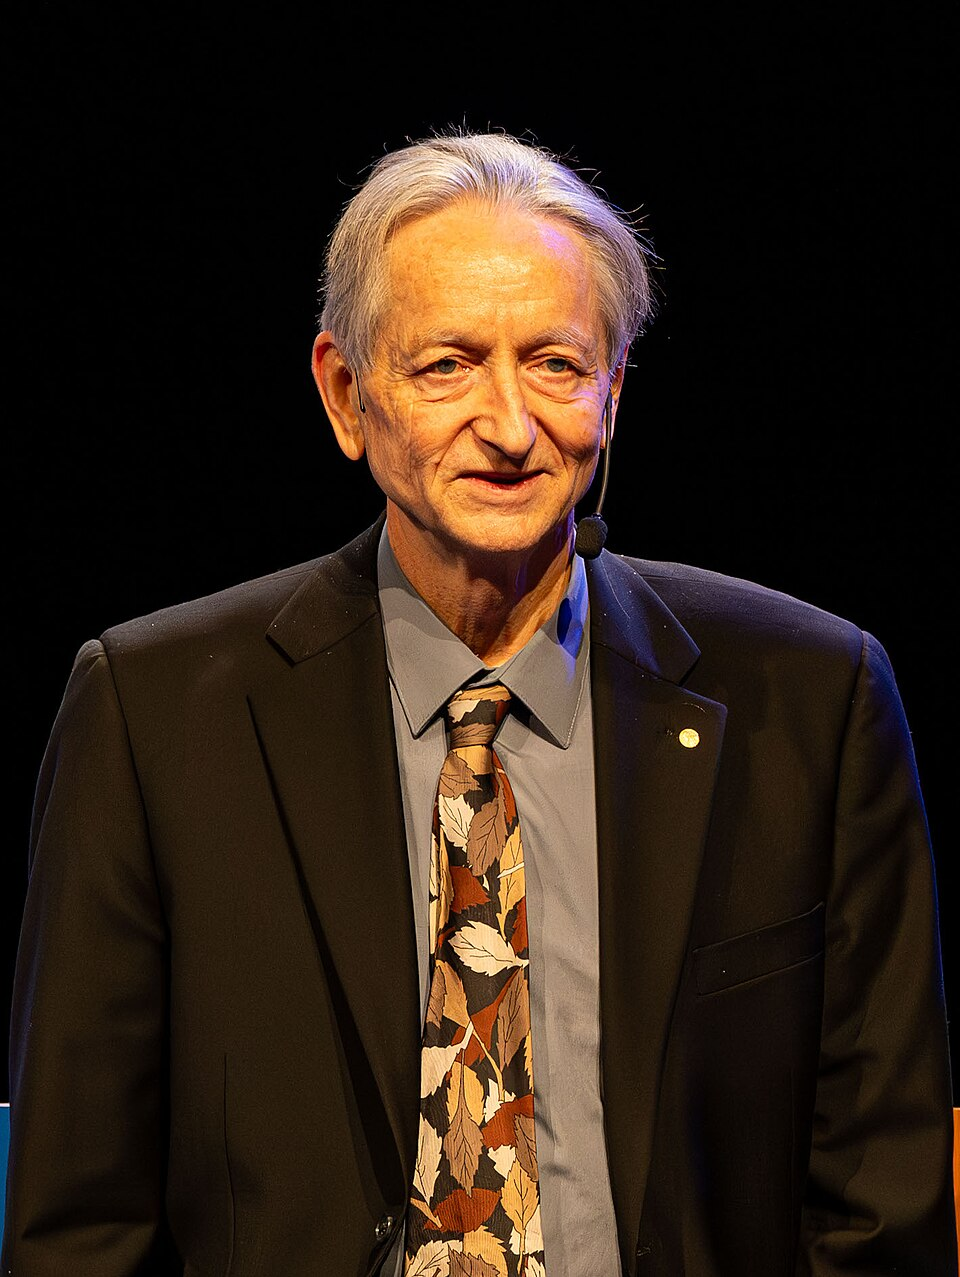
\includegraphics[height=0.48\textheight]{ch12_hinton_2024.jpg}\\[1mm]
\imgcap{Geoffrey Hinton, Premiul Nobel pentru fizică 2024}
\imgcredit{https://commons.wikimedia.org/wiki/File:Geoffrey_E._Hinton,_2024_Nobel_Prize_Laureate_in_Physics_(cropped).jpg}{Foto: Arthur Petron (2024); CC BY-SA 4.0; Wikimedia Commons}
\end{column}
\begin{column}{0.62\textwidth}
\begin{itemize}
    \item \textbf{Statistice}: ARIMA, ETS, HAR, spațiul stărilor: puțini parametri, un model pe serie
    \item \textbf{Machine learning}: regresii penalizate, păduri, boosting pe variabile cu laguri, adesea globale
    \item \textbf{Modele deep de secvențe}: RNN, LSTM, TCN, Transformers, N-BEATS, DeepAR; retropropagarea \refRHW
    \item \textbf{Foundation models}: preantrenate pe multe serii, folosite zero-shot (\atschlink{https://danpele.github.io/Advanced-Time-Series/RO/Cursuri/capitol13_foundation_models_conformal.pdf}{Capitolul 13})
    \item Fiecare generație trebuie să fie mai bună decît cea dinainte în afara eșantionului, cu teste, pe aceleași date
\end{itemize}
\end{column}
\end{columns}
\end{frame}

\begin{frame}{Patru seturi de date, patru tipuri de structură}
\itemsize{\footnotesize}
\begin{center}
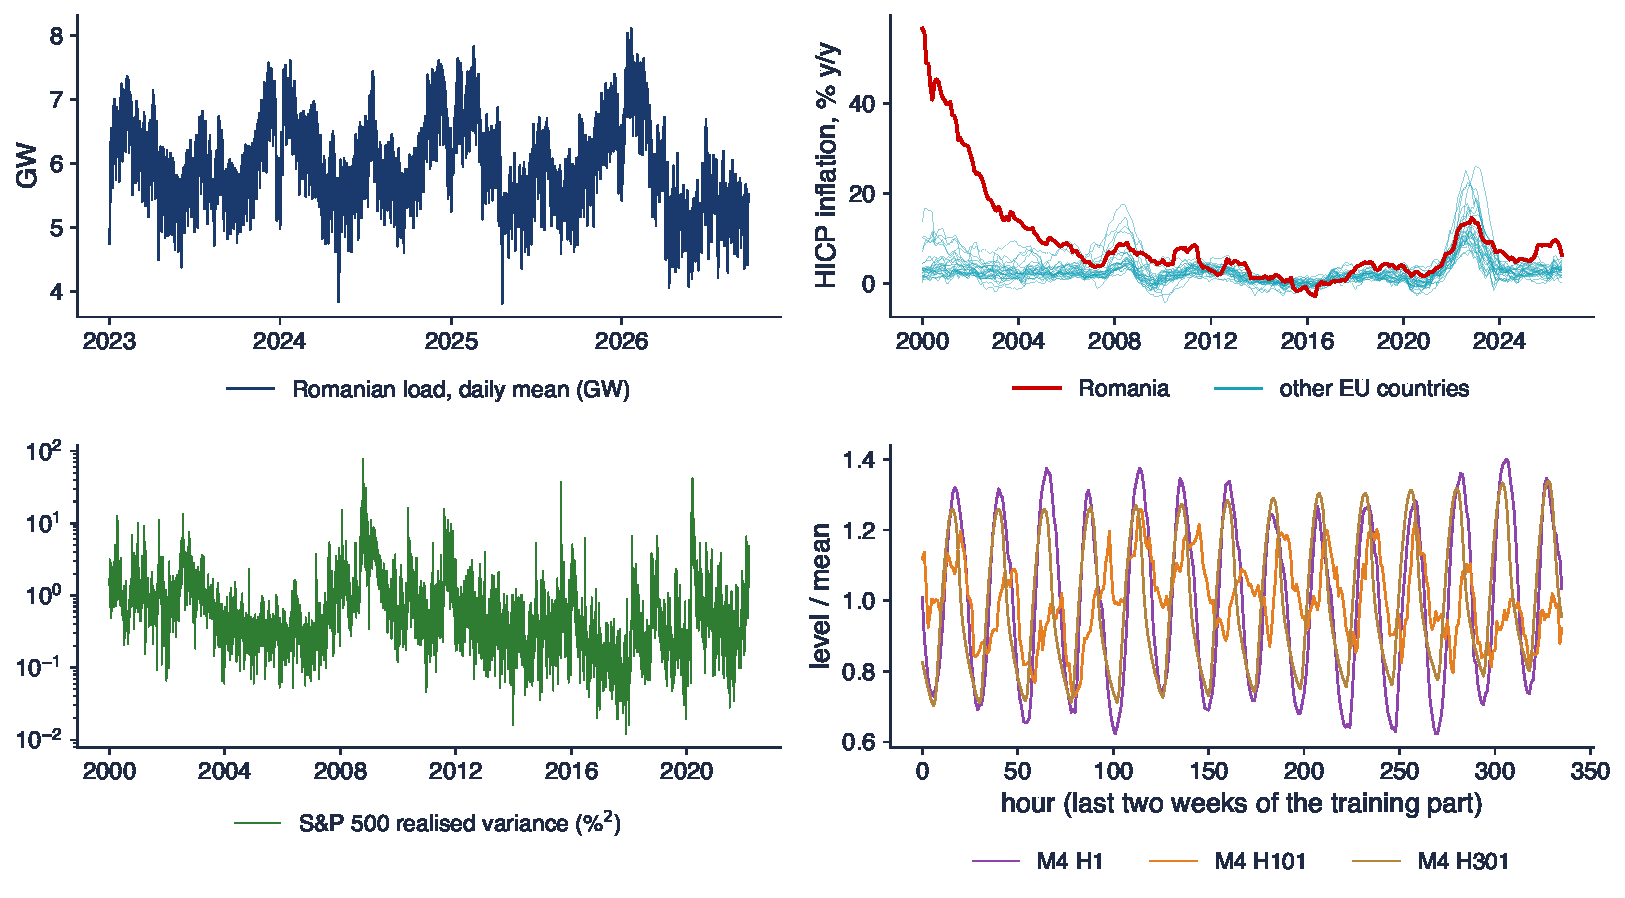
\includegraphics[width=0.97\textwidth,height=0.52\textheight,keepaspectratio]{ats_ch12_overview.pdf}
\end{center}
\vspace{-0.25cm}
\begin{itemize}
    \item Consumul României (media zilnică, în medie 6{,}06 GW); inflația UE (România cu roșu); varianța realizată S\&P 500 (scară logaritmică); trei serii orare M4 (ultimele două săptămîni)
\end{itemize}
\quantlet{ATS\_ch12\_validation}{\qlurl{ATS_ch12_validation}}
\end{frame}

\begin{frame}{Interpretarea celor patru seturi de date}
\itemsize{\small}
\begin{itemize}
    \item Consumul: sezonalitate zilnică și săptămînală puternică, sărbători, ciclu anual lent: o structură de calendar pe care arborii și modelele liniare o captează bine
    \item Inflația: 27 de serii scurte, care se mișcă împreună, cu un șoc comun în 2021--2023: terenul natural pentru modelele globale și pentru panelul în dimensiune mare
    \item Varianța realizată: memorie lungă și cozi groase; reperul HAR din \atschlink{https://danpele.github.io/Advanced-Time-Series/RO/Cursuri/capitol8_volatilitate_avansata.pdf}{Capitolul 8} este greu de depășit
    \item M4 orar: multe serii înrudite de aceeași frecvență, cadrul în care modelele deep globale au cîștigat prima dată
\end{itemize}
\end{frame}


%=============================================================================
\section{Învățarea din date dependente}
%=============================================================================

\begin{frame}{Cunoscut din TSA și elemente noi}
\itemsize{\small}
\begin{itemize}
    \item Cunoscut (\atschlink{https://danpele.github.io/Time-Series-Analysis/RO/Cursuri/capitol9_invatare_automata_serii_timp.pdf}{TSA, Capitolul 9}): variabile cu laguri, validare walk-forward, scurgere de informație prin exemple, ridge și lasso, arbori, păduri aleatoare, gradient boosting, un MLP mic, elemente de predicție conformală, M4 și M5
    \item Nou: statistica din spatele rețetelor
    \begin{itemize}
        \item generalizarea sub mixing; cînd este validă validarea încrucișată; modele globale
        \item consistența selecției și inferența după selecție; păduri cuantilice; boosting cu restricții
        \item gradienți în timp; atenție; dezvoltări în baze de funcții; modele deep cu verosimilitate; interpretare
    \end{itemize}
    \item Replicări: Bergmeir, Hyndman și Koo (2018, secțiunea 4); Montero-Manso și Hyndman (2021) pe inflația UE; protocolul Zeng et al.\ (2023) pe consumul României; evaluarea M4 pe seriile orare
\end{itemize}
\end{frame}

\begin{frame}{Riscul, riscul empiric și diferența de generalizare (1/2)}
\itemsize{\small}
\begin{itemize}
    \item O regulă de prognoză $f$ dintr-o clasă $\mathcal F$ se judecă după pierderea ei așteptată sub legea staționară
    \[ R(f) = \E\,\ell\big(Y_{t+h}, f(X_t)\big), \qquad \hat R_n(f) = \frac1n\sum_{t=1}^n \ell\big(y_{t+h}, f(x_t)\big) \]
    \begin{itemize}
        \item $R(f)$: \textbf{riscul}; $\hat R_n(f)$: \textbf{riscul empiric} pe $n$ perechi de antrenare; $\ell$: pierderea (de exemplu eroarea pătratică); $X_t$: variabilele cunoscute la $t$; $h$: orizontul
    \end{itemize}
    \item Minimizarea riscului empiric (ERM) și diferența de generalizare
    \[ \hat f = \arg\min_{f \in \mathcal F}\hat R_n(f), \qquad R(\hat f) - \hat R_n(\hat f) \le \sup_{f \in \mathcal F}|R(f) - \hat R_n(f)| \]
    \begin{itemize}
        \item diferența: cu cît este mai slabă regula estimată pe date noi decît pe datele de antrenare
    \end{itemize}
\end{itemize}
\end{frame}

\begin{frame}{Riscul, riscul empiric și diferența de generalizare (2/2)}
\itemsize{\small}
\begin{itemize}
    \item Date i.i.d.: abaterea uniformă scade în funcție de complexitatea clasei
    \[ \sup_{\mathcal F}|R - \hat R_n| = O_p\Big(\sqrt{\mathrm{complexitate}(\mathcal F)/n}\Big) \]
    \begin{itemize}
        \item complexitatea: dimensiunea VC sau complexitatea Rademacher, aproximativ numărul de tipare pe care clasa le poate potrivi
    \end{itemize}
    \item Date dependente: cele $n$ observații conțin mai puțină informație; marginea este valabilă cu o \textbf{dimensiune efectivă a eșantionului} mai mică decît $n$
    \begin{itemize}
        \item și numai dacă seria își uită trecutul suficient de repede: mixing
    \end{itemize}
    \item Nestaționaritatea (rupturi, \atschlink{https://danpele.github.io/Advanced-Time-Series/RO/Cursuri/capitol2_rupturi_structurale_modele_neliniare.pdf}{Capitolul 2}) adaugă o a doua diferență: legea viitoare diferă de cea de antrenare; nicio margine nu o acoperă
\end{itemize}
\end{frame}

\begin{frame}{Coeficienții de mixing}
\itemsize{\small}
\begin{itemize}
    \item $\beta$-mixing: cît de departe este viitorul îndepărtat de independența față de trecut
    \[ \beta(a) = \sup_t\,\E\sup_{B\in\sigma(X_{t+a},\dots)}\big|P\big(B\mid\sigma(\dots,X_t)\big) - P(B)\big| \]
    \begin{itemize}
        \item $\sigma(\dots, X_t)$: informația din trecut pînă la $t$; $\sigma(X_{t+a}, \dots)$: evenimentele $B$ din viitor după distanța $a$; $\alpha$-mixing folosește în schimb $|P(A\cap B) - P(A)P(B)|$
        \item mixing: $\beta(a) \to 0$ cînd distanța $a \to \infty$: viitorul îndepărtat este aproape independent de trecut
    \end{itemize}
    \item ARMA staționar cu inovații continue, GARCH și modelele cu schimbare de regim cu lanț ergodic sînt $\beta$-mixing \textbf{geometric}: $\beta(a) \le Cr^a$, $C > 0$, $0 < r < 1$
    \begin{itemize}
        \item memoria lungă (\atschlink{https://danpele.github.io/Advanced-Time-Series/RO/Cursuri/capitol10_memorie_lunga_rough_volatility.pdf}{Capitolul 10}) nu este mixing geometric: dimensiunea efectivă a eșantionului scade mult mai mult
    \end{itemize}
    \item Mixing-ul este presupus, rar testat: este o afirmație despre procesul generator, nu despre eșantion
\end{itemize}
\end{frame}

\begin{frame}{Blocuri și o margine de generalizare}
\itemsize{\small}
\begin{itemize}
    \item \refYu: împărțim eșantionul în $2\mu$ blocuri alternante de lungime $a$; sub $\beta$-mixing, blocurile impare se comportă ca $\mu$ blocuri \textbf{independente}, pînă la o eroare $\mu\,\beta(a)$
    \begin{itemize}
        \item instrumentele i.i.d.\ se aplică apoi cu $\mu = n/(2a)$ observații în loc de $n$
    \end{itemize}
    \item \refMR: pentru un algoritm uniform stabil, cu probabilitatea de cel puțin $1 - \delta$
    \[ R(\hat f) \le \hat R_n(\hat f) + O(\kappa_n a) + O\Big(\sqrt{\log(1/\delta')/\mu}\Big), \qquad \delta' = \delta - 2(\mu - 1)\beta(a) \]
    \begin{itemize}
        \item $\kappa_n$: stabilitatea uniformă, cea mai mare modificare a pierderii cînd se schimbă un punct de antrenare; $\delta$: nivelul de încredere
        \item compromisul în $a$: blocurile lungi fac $\beta(a)$ mic, dar lasă puține blocuri $\mu$; ridge și modelele regularizate sînt uniform stabile, rețelele deep antrenate prin SGD doar aproximativ
    \end{itemize}
    \item Aceeași idee a blocurilor dă bootstrap-ul pe blocuri (\atschlink{https://danpele.github.io/Advanced-Time-Series/RO/Cursuri/capitol0_recapitulare_inferenta.pdf}{Capitolul 0}) și validarea încrucișată pe blocuri
\end{itemize}
\end{frame}

\begin{frame}{Validarea încrucișată pentru serii de timp: schemele}
\itemsize{\small}
\begin{itemize}
    \item \textbf{K subeșantioane aleatoare}: rîndurile matricei de laguri $(y_t; y_{t-1},\dots,y_{t-p})$ repartizate aleator
    \item \textbf{Validarea nedependentă} \refBHK: aceleași subeșantioane, dar rîndurile de antrenare aflate la mai puțin de $p$ laguri de un rînd de test sînt eliminate
    \item \textbf{K blocuri contigue} și \textbf{hv-block} \refBCN, \refRac: blocuri de test contigue, cu un interval de $h$ rînduri (purjare) de fiecare parte
    \item \textbf{În afara eșantionului (OOS)} și \textbf{originea mobilă}: test doar la sfîrșit; singura schemă care imită utilizarea reală, cu prețul unei varianțe mari
    \item Întrebarea nu este care schemă este „corectă”, ci care estimează riscul viitor cu deplasare mică și varianță mică
\end{itemize}
\end{frame}

\begin{frame}{Validitatea validării cu K subeșantioane: Bergmeir, Hyndman și Koo (2018)}
\itemsize{\small}
\begin{itemize}
    \item O autoregresie neliniară cu erori \textbf{necorelate} \refBHK
    \[ y_t = g(y_{t-1},\dots,y_{t-p}; \theta) + \varepsilon_t \]
    \begin{itemize}
        \item $g$: orice funcție de regresie (liniară, arbore, rețea) cu parametrii $\theta$; $p$: numărul de laguri; $\varepsilon_t$: erorile, $\Cov(\varepsilon_t, \varepsilon_s) = 0$ pentru $t \ne s$
        \item rîndurile matricei de laguri sînt atunci suficient de interschimbabile: un rînd de test nu are nicio eroare comună cu un rînd de antrenare
        \item rezultat: estimația MSE prin K subeșantioane este asimptotic nedeplasată și are o varianță mai mică decît OOS, pentru că fiecare rînd este folosit
    \end{itemize}
    \item Eșuează cînd reziduurile sînt autocorelate: un model subspecificat, ținte suprapuse la $h$ pași sau variabile care identifică momentul
    \begin{itemize}
        \item atunci o eroare de test este previzibilă din erorile de antrenare vecine: estimații optimiste
    \end{itemize}
    \item Regula practică: verificați ACF a reziduurilor modelului estimat (Ljung--Box, \atschlink{https://danpele.github.io/Time-Series-Analysis/RO/Cursuri/capitol2_modele_arma.pdf}{TSA, Capitolul 2}) înainte de a avea încredere în K subeșantioane aleatoare
\end{itemize}
\end{frame}

\begin{frame}{Schema replicării: Bergmeir, Hyndman și Koo (2018, secțiunea 4)}
\itemsize{\small}
\begin{itemize}
    \item Serii de lungime 200: 140 de observații de estimare, 60 de evaluare; modele AR(1)--AR(5) prin OLS; prognoze la un pas
    \item Procedurile pe datele de estimare: 5 subeșantioane, LOOCV, validare nedependentă ($p = 5$), OOS (ultimele 20\%); eroarea „adevărată”: modelul pe toate datele de estimare, RMSE pe datele de evaluare
    \item 1\,000 de repetări pentru fiecare proces: AR(3) staționar cu coeficienți aleatori, MA(1) inversabil și un AR sezonier estimat pe decesele accidentale din SUA 1973--1978 ($\phi = 0{,}76$, $\Phi_{12} = 0{,}85$) drept contraexemplu
    \item Precizia și deplasarea fiecărei proceduri
    \[ \mathrm{MAPAE} = \mathrm{media}\,|\widehat{PE} - PE|, \qquad \mathrm{MPAE} = \mathrm{media}\,(\widehat{PE} - PE) \]
    \begin{itemize}
        \item $PE$: eroarea de predicție adevărată (RMSE pe datele de evaluare); $\widehat{PE}$: estimația ei prin procedură; medii pe repetări; MPAE $< 0$: estimare optimistă
    \end{itemize}
\end{itemize}
\end{frame}

\begin{frame}{Precizia și deplasarea schemelor de validare}
\itemsize{\footnotesize}
\begin{center}
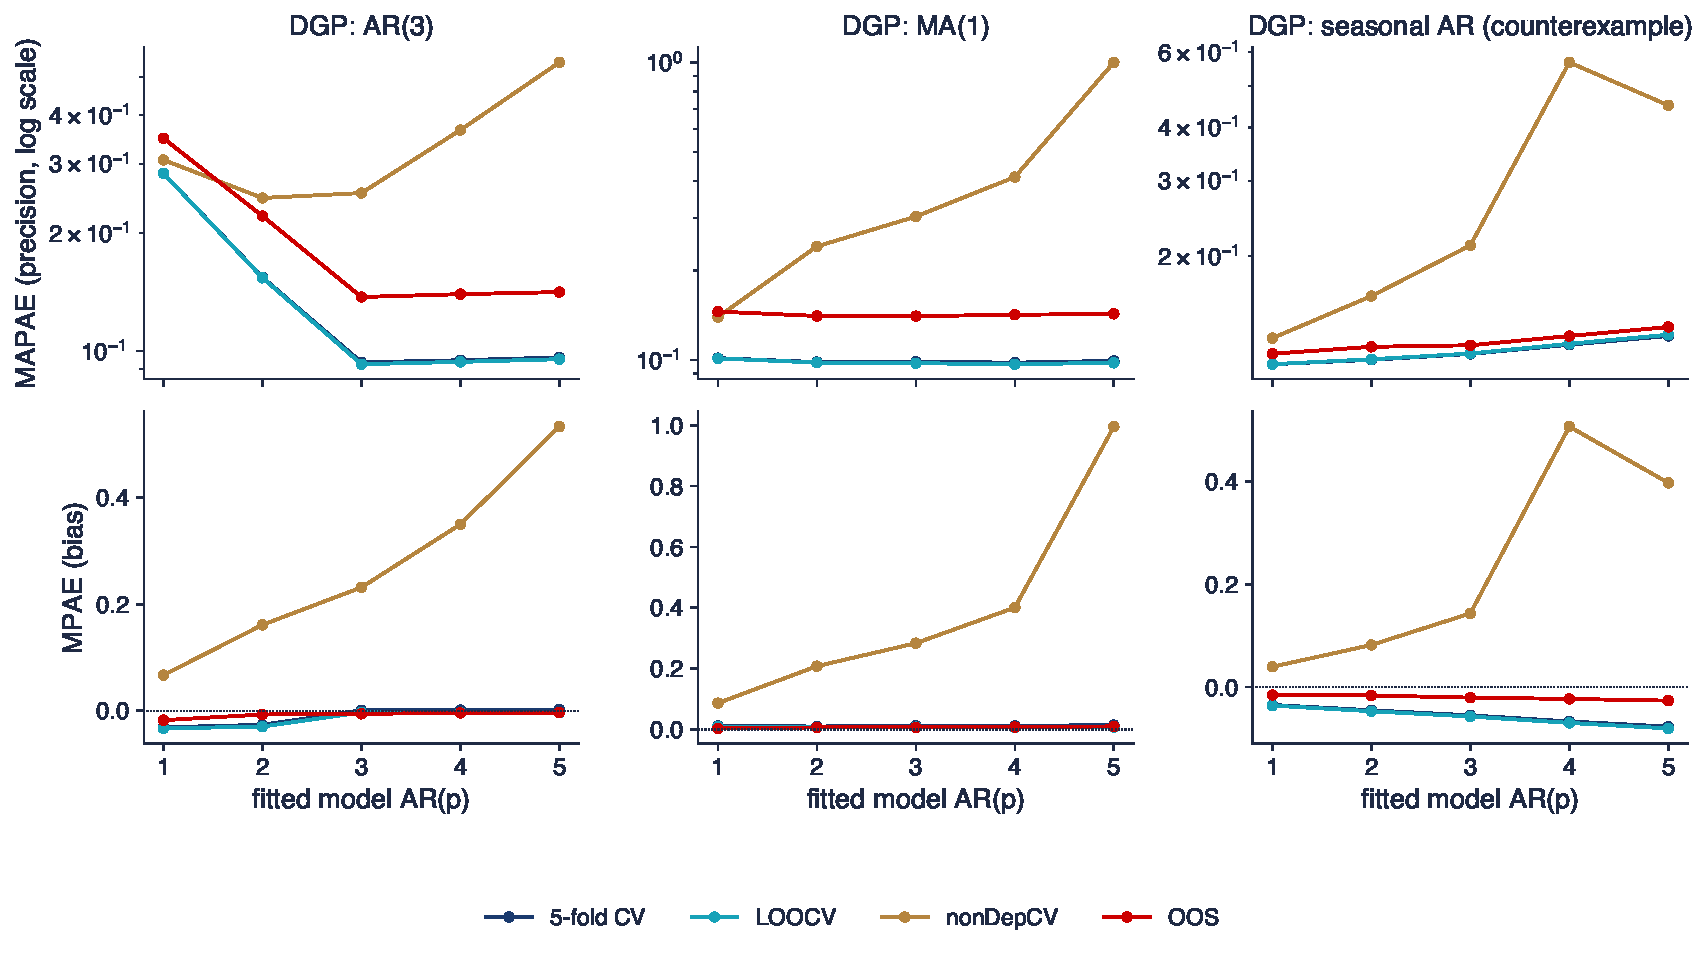
\includegraphics[width=0.97\textwidth,height=0.58\textheight,keepaspectratio]{ats_ch12_cv_bhk.pdf}
\end{center}
\vspace{-0.25cm}
\begin{itemize}
    \item Sus: precizia (scară logaritmică); jos: deplasarea, după ordinul AR estimat și procesul generator
\end{itemize}
\quantlet{ATS\_ch12\_validation}{\qlurl{ATS_ch12_validation}}
\end{frame}

\begin{frame}{Interpretarea replicării}
\itemsize{\small}
\begin{itemize}
    \item Date AR(3), model AR(3): 5 subeșantioane dau MAPAE 0{,}094 față de 0{,}137 pentru OOS, deplasare 0{,}001: ca în lucrare, validarea încrucișată este nedeplasată și mai precisă
    \item AR(1) subspecificat pe date AR(3): reziduurile sînt autocorelate, iar validarea încrucișată își pierde avantajul (MAPAE 0{,}284 față de 0{,}349)
    \item Contraexemplul sezonier: orice AR($p \le 5$) omite lagul 12; validarea încrucișată este deplasată în jos (MPAE \ensuremath{-}0{,}077 pentru AR(5)) și nu mai este mai precisă decît OOS (0{,}130 față de 0{,}136)
    \item Validarea nedependentă elimină atît de multe rînduri încît modelele ei sînt slabe: deplasare 0{,}232 pentru AR(3); prețul independenței se plătește în date
\end{itemize}
\end{frame}

\begin{frame}{Scurgerea de informație prin ținte suprapuse și variabile de timp}
\itemsize{\small}
\begin{itemize}
    \item Ținta $z_t = \frac1h\sum_{j=1}^h y_{t+j}$ (o lună de volatilitate, un trimestru de vînzări): $\mathrm{corr}(z_t, z_{t+1}) \ge (h - 1)/h$ cînd $y$ este zgomot alb, mai mult cînd $y$ este persistent
    \begin{itemize}
        \item un subeșantion aleator pune $z_{t-1}$ și $z_{t+1}$ în antrenare cînd $z_t$ este testat: răspunsul este aproape în setul de antrenare
    \end{itemize}
    \item Un indice de timp sau o variabilă de dată permite unui algoritm flexibil să \textbf{localizeze} rîndul de test între vecinii lui
    \item Simulare: AR(1) cu $\phi = 0{,}9$, $h = 20$, o pădure aleatoare pe $y_t,\dots,y_{t-4}$ și un indice de timp; 60 de repetări; raportul dintre RMSE estimat și RMSE adevărat pe date noi
\end{itemize}
\end{frame}

\begin{frame}{Optimismul fiecărei scheme de validare}
\itemsize{\footnotesize}
\begin{center}
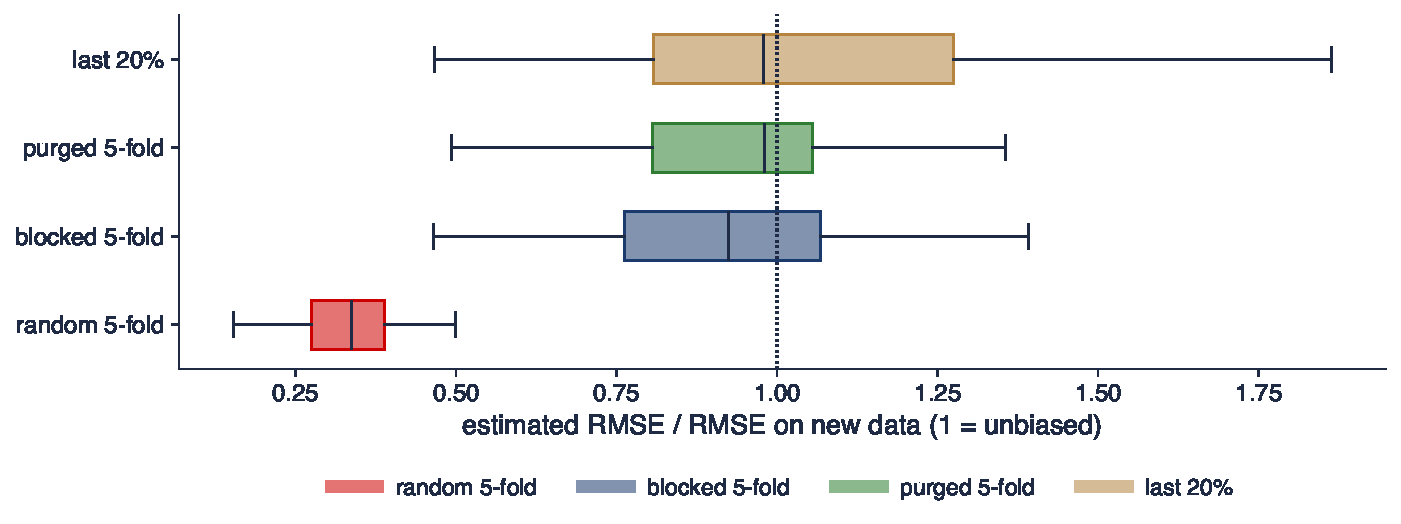
\includegraphics[width=0.97\textwidth,height=0.46\textheight,keepaspectratio]{ats_ch12_leakage.pdf}
\end{center}
\vspace{-0.25cm}
\begin{itemize}
    \item Raportul 1: schema estimează fără deplasare eroarea pe date noi; sub 1: optimistă
\end{itemize}
\quantlet{ATS\_ch12\_validation}{\qlurl{ATS_ch12_validation}}
\end{frame}

\begin{frame}{Interpretarea experimentului de scurgere}
\itemsize{\small}
\begin{itemize}
    \item 5 subeșantioane aleatoare: raportul median 0{,}34 (quartile 0{,}28--0{,}39): pretinde o eroare de trei ori mai mică decît cea reală
    \item 5 blocuri contigue 0{,}92, 5 blocuri cu purjare 0{,}98, ultimele 20\% 0{,}98: contiguitatea și purjarea elimină cea mai mare parte a deplasării
    \item Blocurile interioare lasă încă pădurea să interpoleze în timp; doar ultimul bloc reproduce extrapolarea în viitor
    \item Regula: purjați cel puțin $h$ rînduri în jurul fiecărui bloc de test și eliminați indicii de timp, cu excepția cazului în care trendul este modelat explicit
\end{itemize}
\end{frame}

\begin{frame}{Recapitulare: învățarea din date dependente}
\itemsize{\small}
\begin{itemize}
    \item Marginile de generalizare sînt valabile cu o dimensiune efectivă a eșantionului dată de mixing; blocurile sînt instrumentul comun
    \item Validarea cu K subeșantioane aleatoare este validă pentru autoregresii cu erori necorelate și atunci este mai bună decît OOS
    \item Țintele suprapuse, subspecificarea și variabilele de timp o strică: blocuri, purjare și o perioadă finală neatinsă
\end{itemize}
\end{frame}


%=============================================================================
\section{Modele globale și regresie în dimensiune mare}
%=============================================================================

\begin{frame}{Modele locale și modele globale}
\itemsize{\small}
\begin{itemize}
    \item \textbf{Local}: un model pentru fiecare serie, $\hat y_{i,t+h} = f_i(y_{i,t}, y_{i,t-1},\dots)$; \textbf{global}: o singură funcție pentru toate seriile, $\hat y_{i,t+h} = f(y_{i,t}, y_{i,t-1},\dots)$
    \begin{itemize}
        \item modelele globale reunesc $N \times T$ rînduri: mult mai multe date pe parametru
    \end{itemize}
    \item \refMMH: pentru orice mulțime de serii există un model global care prognozează la fel de bine ca modelele locale; modelele globale își permit \textbf{memorie mai lungă} și complexitate mai mare
    \begin{itemize}
        \item marginea lor: complexitatea unui model global crește cu $NT$, cea a $N$ modele locale cu cîte $T$
    \end{itemize}
    \item Cîștigătorii M4 și M5 au fost globali (\refSmyl; LightGBM în \refMfiveA): reunirea datelor, nu adîncimea, a fost ingredientul comun
    \item Scalarea contează: seriile de niveluri diferite se împart la propria scală înainte de reunire (ratele inflației au aceeași scală)
\end{itemize}
\end{frame}

\begin{frame}{Schema studiului: inflația UE, local față de global}
\itemsize{\small}
\begin{itemize}
    \item Inflația anuală IAPC a celor 27 de țări UE; prognoze directe la $h = 1$ și $h = 12$ luni din modele AR($p$), $p \in \{1, 2, 3, 6, 12, 18, 24, 36\}$
    \item Fereastră mobilă de 120 de luni; origini ale prognozei din ianuarie 2015 (139 origini pentru $h = 1$)
    \item Local: 27 de regresii OLS pentru fiecare origine; global: o singură regresie OLS reunită (aceiași coeficienți pentru toate țările), ca în \refMMH
    \item Pierderea: RMSE în puncte procentuale; testul DM pe diferența medie a pierderilor dintre țări (corecția HLN, \atschlink{https://danpele.github.io/Advanced-Time-Series/RO/Cursuri/capitol1_evaluarea_prognozelor.pdf}{Capitolul 1})
\end{itemize}
\end{frame}

\begin{frame}{Memoria ajută modelele globale și le afectează pe cele locale}
\itemsize{\footnotesize}
\begin{center}
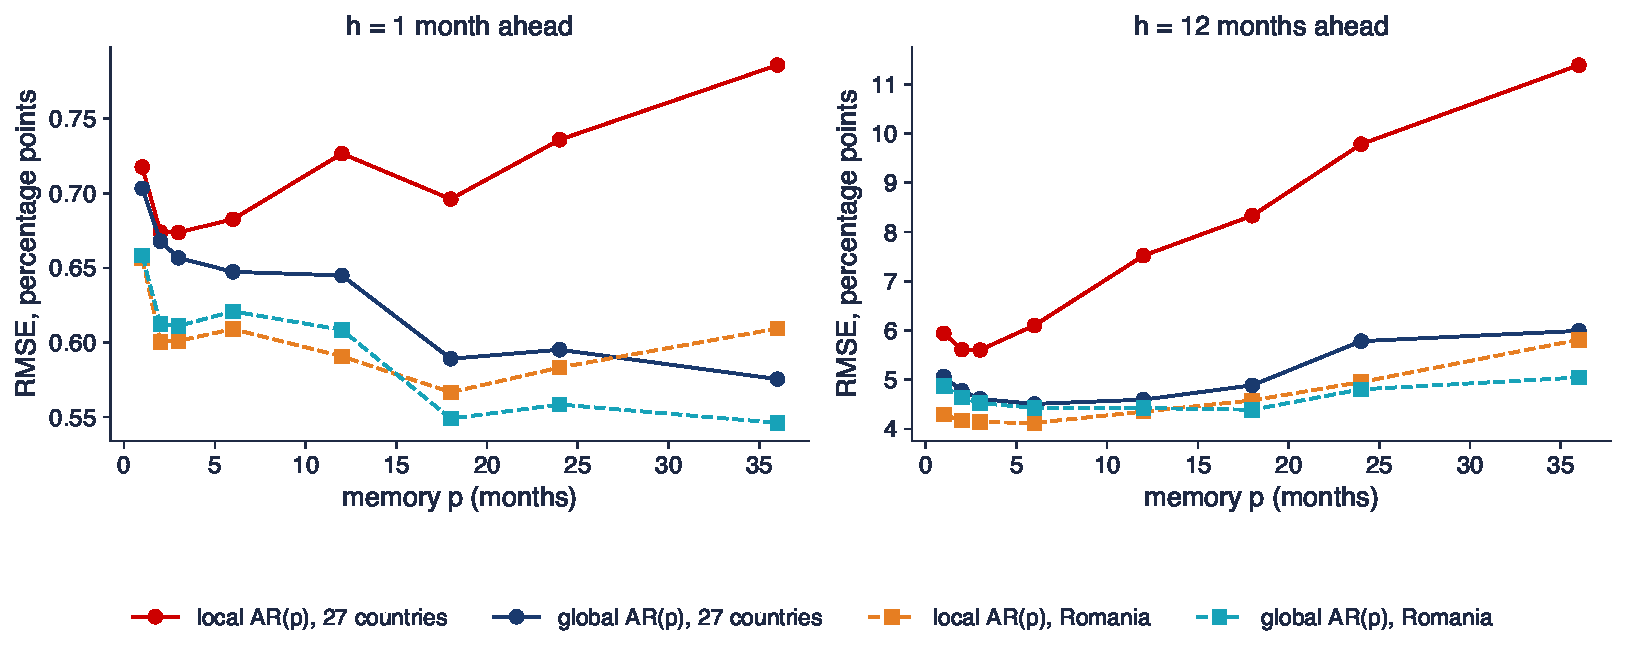
\includegraphics[width=0.97\textwidth,height=0.5\textheight,keepaspectratio]{ats_ch12_global_local.pdf}
\end{center}
\vspace{-0.25cm}
\begin{itemize}
    \item RMSE în funcție de memoria $p$; cercuri: media celor 27 de țări; pătrate: România
\end{itemize}
\quantlet{ATS\_ch12\_global\_models}{\qlurl{ATS_ch12_global_models}}
\end{frame}

\begin{frame}{Interpretarea modelelor locale și globale}
\itemsize{\small}
\begin{itemize}
    \item $h = 1$: RMSE local este minim la $p = 3$ (0{,}67), apoi se deteriorează; cel global scade pînă la $p = 36$ (0{,}58); DM pe media celor 27 de țări \ensuremath{-}4{,}40 ($p$ $<$0{,}001)
    \item $h = 12$: valul din 2021--2023 domină; AR(36) local ajunge la 11{,}39 față de 5{,}99 global; cel mai bun global 4{,}51 față de cel mai bun local 5{,}60, DM \ensuremath{-}1{,}09 ($p$ 0{,}277)
    \item România separat: modelul global ajută la $h = 1$ cu memorie lungă (0{,}55 față de 0{,}61 la $p = 36$), nesemnificativ (DM $p$ 0{,}19)
    \item Lecția lui Montero-Manso și Hyndman se confirmă: reunirea datelor permite o memorie mai lungă; pentru o singură serie, cîștigul este real, dar greu de demonstrat
\end{itemize}
\end{frame}

\begin{frame}{Lasso (1/2): condițiile de optimalitate}
\itemsize{\small}
\begin{itemize}
    \item \refTib: cele mai mici pătrate cu o penalizare $\ell_1$
    \[ \hat\beta = \arg\min_\beta \frac1{2n}\|y - X\beta\|^2 + \lambda\|\beta\|_1, \qquad \|\beta\|_1 = \sum_j|\beta_j| \]
    \begin{itemize}
        \item $y$: ținta, $n \times 1$; $X$: predictorii, $n \times p$, cu coloanele $x_j$; $\lambda \ge 0$: penalizarea; cu cît este mai mare, cu atît mai mulți coeficienți devin zero
        \item condițiile Karush--Kuhn--Tucker (KKT): $\frac1n x_j'(y - X\hat\beta) = \lambda\,\mathrm{sign}(\hat\beta_j)$ dacă $\hat\beta_j \ne 0$ și $|\frac1n x_j'(y - X\hat\beta)| \le \lambda$ altfel
    \end{itemize}
    \item Predictori ortonormali ($X'X = nI$): pragul moale aplicat coeficientului OLS $z_j$
    \[ \hat\beta_j^{\mathrm{lasso}} = \mathrm{sign}(z_j)\,(|z_j| - \lambda)_+, \qquad \hat\beta_j^{\mathrm{ridge}} = \frac{z_j}{1 + \lambda} \]
    \begin{itemize}
        \item $(u)_+ = \max(u, 0)$; lasso selectează (anulează coeficienții $z_j$ mici), ridge doar îi micșorează
    \end{itemize}
\end{itemize}
\end{frame}

\begin{frame}{Lasso (2/2): predicție și selecție}
\itemsize{\small}
\begin{itemize}
    \item Predicția: cu $s$ coeficienți nenuli și o valoare proprie restrînsă $\kappa$, pentru $\lambda \asymp \sigma\sqrt{\log p/n}$
    \[ \frac1n\|X(\hat\beta - \beta)\|^2 = O_p\Big(\frac{s\log p}{n\kappa^2}\Big) \]
    \begin{itemize}
        \item $\sigma$: abaterea standard a erorii; $\kappa$: cît de departe este $X$ de colinearitate pe direcțiile rare; serii de timp: aceeași rată pentru VAR stabile \refBM, erori cu cozi groase \refMM
    \end{itemize}
    \item Selecția este mai grea decît predicția: consistența semnelor cere \textbf{condiția de nereprezentare} \refZY
    \[ \big\|X_{S^c}'X_S(X_S'X_S)^{-1}\mathrm{sign}(\beta_S)\big\|_\infty < 1 \]
    \begin{itemize}
        \item $S$: mulțimea predictorilor relevanți, $S^c$: ceilalți; eșuează cînd predictorii relevanți și irelevanți sînt corelați (țări vecine, laguri)
    \end{itemize}
\end{itemize}
\end{frame}

\begin{frame}{Lasso adaptiv și elastic net}
\itemsize{\small}
\begin{itemize}
    \item \textbf{Lasso adaptiv} \refZou: ponderi specifice fiecărui coeficient, dintr-o estimație de prima etapă
    \[ \lambda\sum_j w_j|\beta_j|, \qquad w_j = 1/|\tilde\beta_j|^\gamma \]
    \begin{itemize}
        \item $\tilde\beta_j$: estimația de prima etapă (OLS, ridge); $\gamma > 0$; coeficienții mari sînt penalizați puțin, cei mici mult
        \item \textbf{proprietatea de oracol}: selecție consistentă și estimații $\sqrt n$-normale ale coeficienților nenuli, fără condiția de nereprezentare
    \end{itemize}
    \item \textbf{Elastic net} \refZH: o combinație a penalizărilor lasso și ridge
    \[ \lambda\Big(\alpha\|\beta\|_1 + \frac{1 - \alpha}2\|\beta\|_2^2\Big) \]
    \[ \hat\beta_j = \frac{\mathrm{sign}(z_j)(|z_j| - \lambda\alpha)_+}{1 + \lambda(1 - \alpha)} \ (X'X = nI) \]
    \begin{itemize}
        \item $\alpha \in [0, 1]$: $\alpha = 1$ lasso, $\alpha = 0$ ridge; efectul de grup: predictorii corelați intră împreună, în loc să fie ales unul la întîmplare
    \end{itemize}
    \item Penalizarea se alege prin validare încrucișată: cu ținte la $h$ pași folosiți blocuri cu purjare de $h$ perioade (secțiunea 1)
\end{itemize}
\end{frame}

\begin{frame}{Inferența după selecție}
\itemsize{\small}
\begin{itemize}
    \item Practica naivă: selecție cu lasso, apoi raportarea statisticilor $t$ OLS ale variabilelor selectate: p-value-urile sînt \textbf{prea mici}
    \begin{itemize}
        \item aceleași date au ales modelul și îl testează: distribuția lui $\hat\beta$ este condiționată de faptul că a fost selectat
    \end{itemize}
    \item Remedii: intervale \textbf{PoSI}, valabile pentru orice selecție \refBerk; intervale \textbf{condiționate exacte} pentru lasso (un eveniment de selecție poliedral) \refLSST
    \item Pentru un coeficient de interes (o dobîndă de politică, un șoc extern): \textbf{dubla selecție} \refBCH: lasso al lui $y$ pe variabilele de control, lasso al regresorului de interes pe aceleași variabile, OLS pe reuniune
    \begin{itemize}
        \item cu erori standard HAC pentru serii de timp (\atschlink{https://danpele.github.io/Advanced-Time-Series/RO/Cursuri/capitol0_recapitulare_inferenta.pdf}{Capitolul 0})
    \end{itemize}
    \item Pentru prognoză, selecția este un mijloc: se judecă după pierderea în afara eșantionului și după stabilitatea a ceea ce este selectat
\end{itemize}
\end{frame}

\begin{frame}{Schema studiului: inflația României din panelul UE}
\itemsize{\small}
\begin{itemize}
    \item Ținta: inflația anuală IAPC a României peste 12 luni; fereastră de 120 de luni, reestimare la fiecare 3 luni; 128 de prognoze (ianuarie 2016 -- august 2026)
    \item Variabile: 3 laguri proprii (nepenalizate) și 3 laguri ale celorlalte 26 de țări: 78 predictori penalizați pentru circa 105 observații
    \item Modele: AR(3) (reper), ridge, lasso, lasso adaptiv, elastic net ($\alpha = 0{,}5$), OLS după lasso, AR(12) global al panelului; penalizarea prin 5 blocuri cu purjare de 12 luni
    \item Literatura despre prognoza inflației cu multe date \refMVVZ, \refGCLSS, aplicată aici pe panelul UE
\end{itemize}
\end{frame}

\begin{frame}{Selecția lasso pe panel și acuratețea ei}
\itemsize{\footnotesize}
\begin{center}
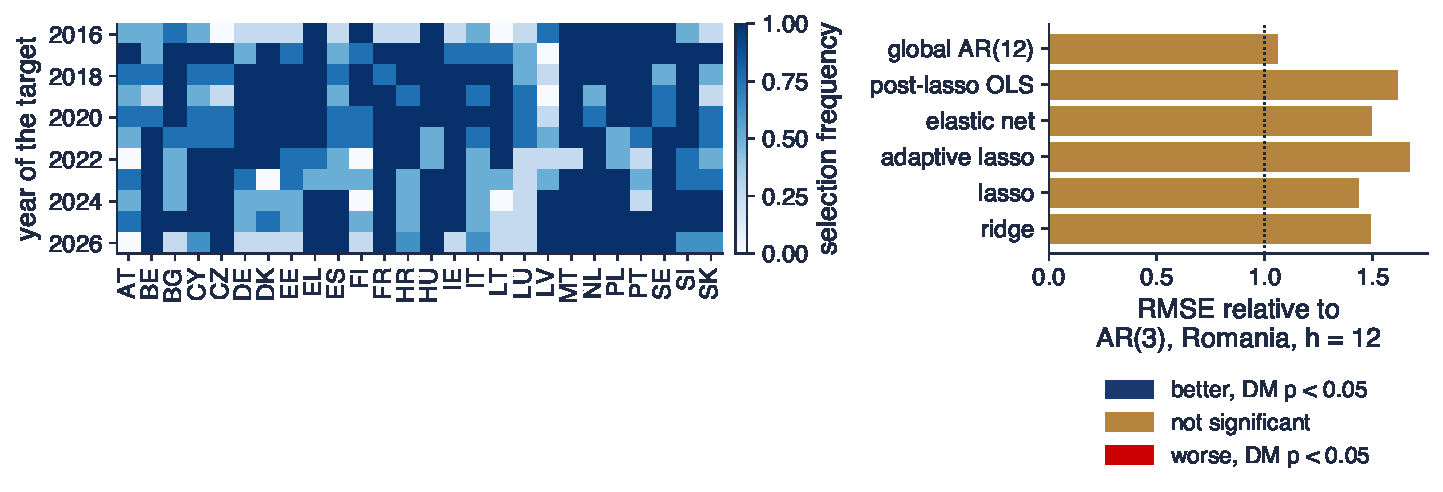
\includegraphics[width=0.97\textwidth,height=0.48\textheight,keepaspectratio]{ats_ch12_ro_lasso.pdf}
\end{center}
\vspace{-0.25cm}
\begin{itemize}
    \item Stînga: ponderea originilor din fiecare an în care o țară intră în lasso; dreapta: RMSE relativ la AR(3), culoarea după testul DM
\end{itemize}
\quantlet{ATS\_ch12\_global\_models}{\qlurl{ATS_ch12_global_models}}
\end{frame}

\begin{frame}{Interpretarea lasso pe panel}
\itemsize{\small}
\begin{itemize}
    \item Selecția este instabilă: mediana de 34 din 78 predictori (între 15 și 61); cele mai frecvente sînt EL, NL, MT, nu vecinii României
    \item Acuratețea: RMSE AR(3) 4{,}13; lasso de 1{,}44 ori, lasso adaptiv de 1{,}67 ori, elastic net de 1{,}49 ori, ridge de 1{,}49 ori mai mare; AR(12) global 1{,}06
    \item Niciuna dintre diferențe nu este semnificativă (DM $p$ între 0{,}20 și 0{,}39): circa 10 perioade independente de 12 luni, una dominată de valul din 2022
    \item Dimensiune mare cu 105 observații ale unei ținte persistente: validarea alege penalizări mici, panelul potrivește co-mișcări trecute care nu se repetă; aici cîștigă parcimonia
\end{itemize}
\end{frame}

\begin{frame}{Recapitulare: modele globale și dimensiune mare}
\itemsize{\small}
\begin{itemize}
    \item Modelele globale reunesc multe serii și își permit memorie lungă; pe inflația UE cîștigă la o lună
    \item Lasso prognozează bine sub raritate și valori proprii restrînse; selectează bine doar sub condiția de nereprezentare; lasso adaptiv și elastic net o relaxează
    \item Raportați stabilitatea selecției și folosiți inferența PoSI, exactă sau prin dubla selecție, niciodată statisticile $t$ naive
\end{itemize}
\end{frame}


%=============================================================================
\section{Ansambluri de arbori în profunzime}
%=============================================================================

\begin{frame}{Bagging: varianța unei medii}
\itemsize{\small}
\begin{itemize}
    \item Media a $B$ predictori $\hat f_b(x)$ antrenați pe eșantioane bootstrap \refBreA
    \[ \Var\Big(\frac1B\sum_{b=1}^B\hat f_b(x)\Big) = \frac1{B^2}\big(B\sigma^2 + B(B - 1)\rho\sigma^2\big) = \rho\sigma^2 + \frac{1 - \rho}B\sigma^2 \]
    \begin{itemize}
        \item $\sigma^2$: varianța unui singur predictor; $\rho$: corelația dintre doi predictori (după date și randomizare)
        \item mai mulți arbori elimină doar al doilea termen; pragul $\rho\sigma^2$ scade doar prin \textbf{decorelarea} arborilor
    \end{itemize}
    \item \textbf{Pădurile aleatoare} \refBreB: un subset aleator de $m_{\mathrm{try}}$ variabile la fiecare ramificare scade $\rho$, cu prețul unei deplasări mici
    \begin{itemize}
        \item teorie: consistența pentru regresia aditivă \refSBV; arborii onești (eșantioane separate pentru ramificări și valorile din frunze) dau prognoze asimptotic normale \refWA
    \end{itemize}
    \item Arborii nu pot extrapola: o prognoză este o medie a țintelor trecute, deci trendurile și salturile de nivel cer diferențiere sau o parte liniară
\end{itemize}
\end{frame}

\begin{frame}{Păduri de regresie cuantilică}
\itemsize{\small}
\begin{itemize}
    \item \refMei: păstrăm \textbf{toate} țintele de antrenare în frunze și le ponderăm după cît de des împart o frunză cu $x$
    \[ w_i(x) = \frac1B\sum_{b=1}^B \frac{\mathbf 1\{x_i \in L_b(x)\}}{|L_b(x)|}, \qquad \hat F(y\mid x) = \sum_i w_i(x)\,\mathbf 1\{y_i \le y\} \]
    \begin{itemize}
        \item $L_b(x)$: frunza arborelui $b$ care conține $x$; $|L_b(x)|$: numărul punctelor de antrenare din ea; $\sum_i w_i(x) = 1$
        \item $\hat F(y\mid x)$: funcția de repartiție condiționată estimată; cuantila $\hat q_\tau(x) = \inf\{y: \hat F(y\mid x) \ge \tau\}$
    \end{itemize}
    \item Aceeași pădure dă toate cuantilele: fără încrucișări, fără reestimare pentru fiecare nivel
    \begin{itemize}
        \item consistentă pentru distribuția condiționată, în condiții de regularitate; o pădure aleatoare este o metodă adaptivă de tip vecini apropiați
    \end{itemize}
    \item Evaluarea prin pierderea pinball și acoperire (\atschlink{https://danpele.github.io/Advanced-Time-Series/RO/Cursuri/capitol1_evaluarea_prognozelor.pdf}{Capitolul 1}): benzile sînt corecte doar dacă pădurea a fost antrenată pe date asemănătoare viitorului
\end{itemize}
\end{frame}

\begin{frame}{Gradient boosting (1/2): coborîre pe gradient în spațiul funcțiilor}
\itemsize{\small}
\begin{itemize}
    \item \refFri: se adaugă arbori mici, fiecare ajustat pe gradientul negativ al pierderii în punctul curent
    \[ F_m = F_{m-1} + \nu\,h_m, \qquad g_i = -\frac{\partial\ell(y_i, F)}{\partial F}\Big|_{F = F_{m-1}(x_i)} \]
    \begin{itemize}
        \item $F_m$: funcția estimată după $m$ arbori; $h_m$: un arbore mic ajustat pe $(x_i, g_i)$; $\nu \in (0, 1]$: rata de învățare (shrinkage): pași mai mici, mai mulți arbori, varianță mai mică
        \item pierderea pătratică: $g_i$ = reziduul; pierderea pinball: $g_i = \tau - \mathbf 1\{y_i < F\}$ (boosting cuantilic)
    \end{itemize}
\end{itemize}
\end{frame}

\begin{frame}{Gradient boosting (2/2): ordinul doi, histograme, restricții}
\itemsize{\small}
\begin{itemize}
    \item Ordinul doi \refCG: valoarea optimă a unei frunze și cîștigul unei ramificări
    \[ w^* = -\frac{G}{H + \lambda}, \qquad \text{cîștigul} = \frac12\Big[\frac{G_L^2}{H_L + \lambda} + \frac{G_R^2}{H_R + \lambda} - \frac{G^2}{H + \lambda}\Big] - \gamma \]
    \begin{itemize}
        \item $G$, $H$: sumele derivatelor de ordinul întîi și doi ale pierderii pe punctele unei frunze ($L$, $R$: descendentul stîng și drept); $\lambda$: penalizarea valorilor frunzelor; $\gamma$: costul unei ramificări
    \end{itemize}
    \item LightGBM \refKeA: variabile grupate în histograme (cel mult 255 de intervale), creștere pe frunze, eșantionare unilaterală după gradient; HistGradientBoosting din scikit-learn (folosit aici) urmează aceeași construcție
    \item Restricțiile de monotonie: o ramificare este permisă doar dacă valorile frunzelor stîngă și dreaptă respectă ordinea, iar descendenții moștenesc limitele; funcția estimată este atunci monotonă în acea variabilă peste tot
\end{itemize}
\end{frame}

\begin{frame}{Schema studiului: consumul României pentru ziua următoare}
\itemsize{\small}
\begin{columns}[T]
\begin{column}{0.34\textwidth}
\centering
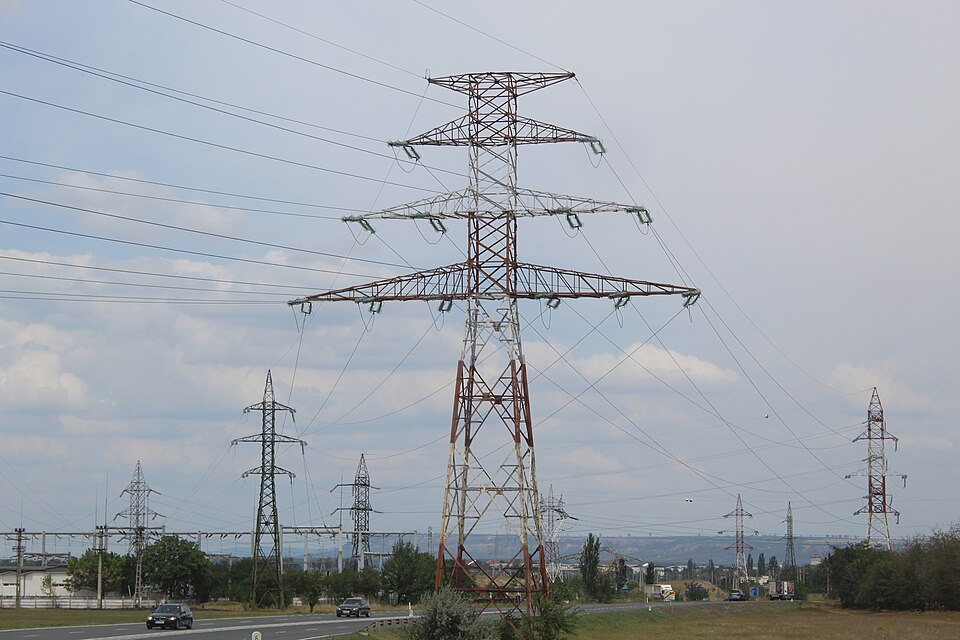
\includegraphics[height=0.42\textheight]{ch12_marasesti_750kv_2022.jpg}\\[1mm]
\imgcap{Linie de 750 kV la Mărășești, România}
\imgcredit{https://commons.wikimedia.org/wiki/File:750_kV_electricity_tower_at_M\%C4\%83r\%C4\%83\%C8\%99e\%C8\%99ti,_Romania.jpg}{Foto: TrainSimFan (2022); CC BY-SA 4.0; Wikimedia Commons}
\end{column}
\begin{column}{0.64\textwidth}
\begin{itemize}
    \item Prognozăm cele 24 de valori orare ale zilei $d + 1$ cu date pînă în ziua $d$; evaluare pe 638 de zile, ianuarie 2025 -- septembrie 2026
    \item Reper: ARX-ul expert din \atschlink{https://danpele.github.io/Advanced-Time-Series/RO/Cursuri/capitol1_evaluarea_prognozelor.pdf}{Capitolul 1} (\refZW): o regresie pe oră, fereastră de 364 de zile, reestimat zilnic
    \item Algoritmi globali (un model pentru toate orele) pe aceleași laguri, ora, ziua săptămînii, sărbătorile din România, ciclul anual; reestimați lunar pe toate datele anterioare: RF cu benzi QRF, HGB, HGB crescător în cele trei laguri ale consumului, HGB cuantilic
    \item Pierderi: MAE, pinball mediu pe decile, acoperirea de 80\%; DM față de ARX și MCS (\atschlink{https://danpele.github.io/Advanced-Time-Series/RO/Cursuri/capitol1_evaluarea_prognozelor.pdf}{Capitolul 1})
\end{itemize}
\end{column}
\end{columns}
\end{frame}

\begin{frame}{Arbori față de ARX-ul expert}
\itemsize{\footnotesize}
\begin{center}
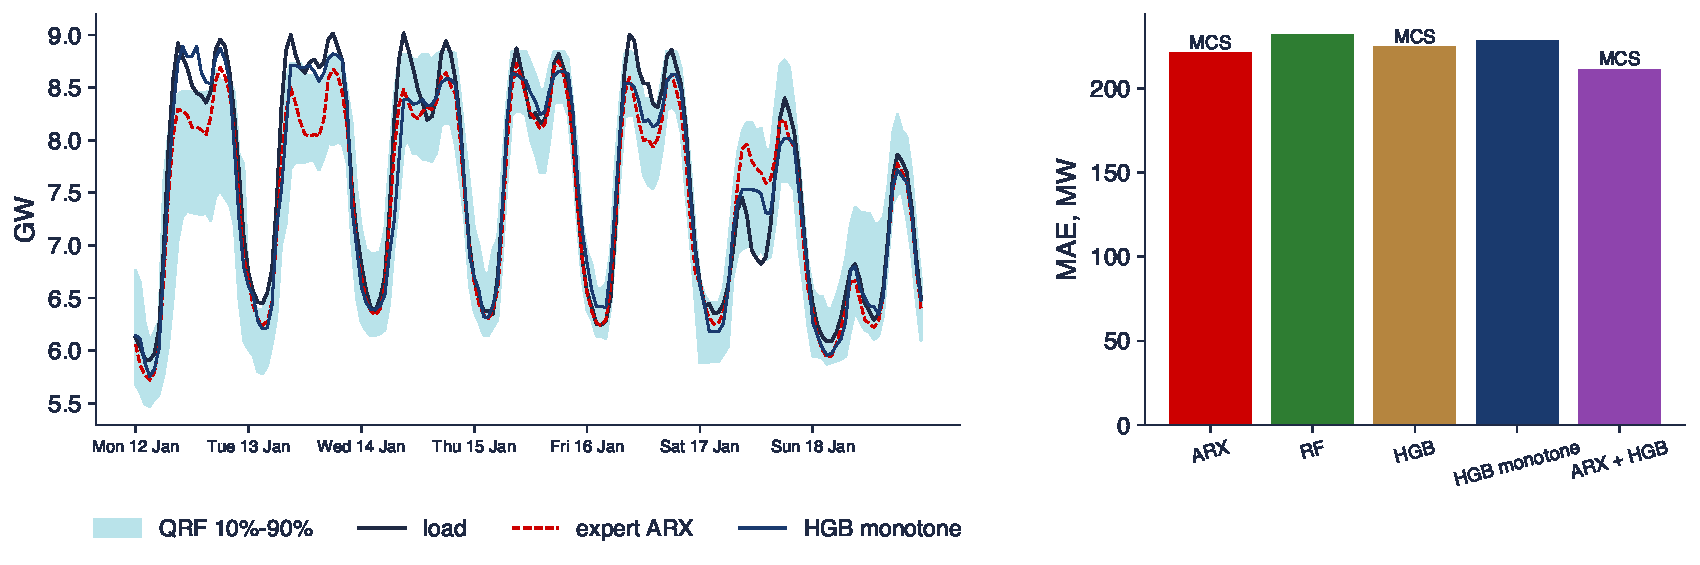
\includegraphics[width=0.97\textwidth,height=0.46\textheight,keepaspectratio]{ats_ch12_load_trees.pdf}
\end{center}
\vspace{-0.25cm}
\begin{itemize}
    \item Stînga: o săptămînă din ianuarie cu benzile QRF 10\%--90\%; dreapta: MAE în MW, MCS marchează modelele din mulțimea de încredere de 90\%
\end{itemize}
\quantlet{ATS\_ch12\_trees}{\qlurl{ATS_ch12_trees}}
\end{frame}

\begin{frame}{Interpretarea comparației pentru consum}
\itemsize{\small}
\begin{itemize}
    \item MAE (MW): ARX 221, RF 232, HGB 225, HGB monoton 228; pădurea este semnificativ mai slabă (DM 2{,}84), boosting nu diferă semnificativ de ARX
    \item Media egală dintre ARX și boosting: 211 MW, DM \ensuremath{-}3{,}36 ($p$ $<$0{,}001), singurul model din MCS: combinarea este mai bună decît selecția (\atschlink{https://danpele.github.io/Advanced-Time-Series/RO/Cursuri/capitol1_evaluarea_prognozelor.pdf}{Capitolul 1})
    \item Cuantile: pinball (MW) ARX 89{,}1, HGB cuantilic 89{,}5, QRF 92{,}8; acoperirea de 80\%: 78\%, 61\%, 83\%: boosting-ul cuantilic este îngust, dar acoperă prea puțin, QRF acoperă prea mult
    \item Un model liniar reestimat zilnic, cu structura corectă, este un reper puternic; arborii aduc valoare ca o completare, nu ca un înlocuitor
\end{itemize}
\end{frame}

\begin{frame}{Restricțiile de monotonie în practică}
\itemsize{\footnotesize}
\begin{center}
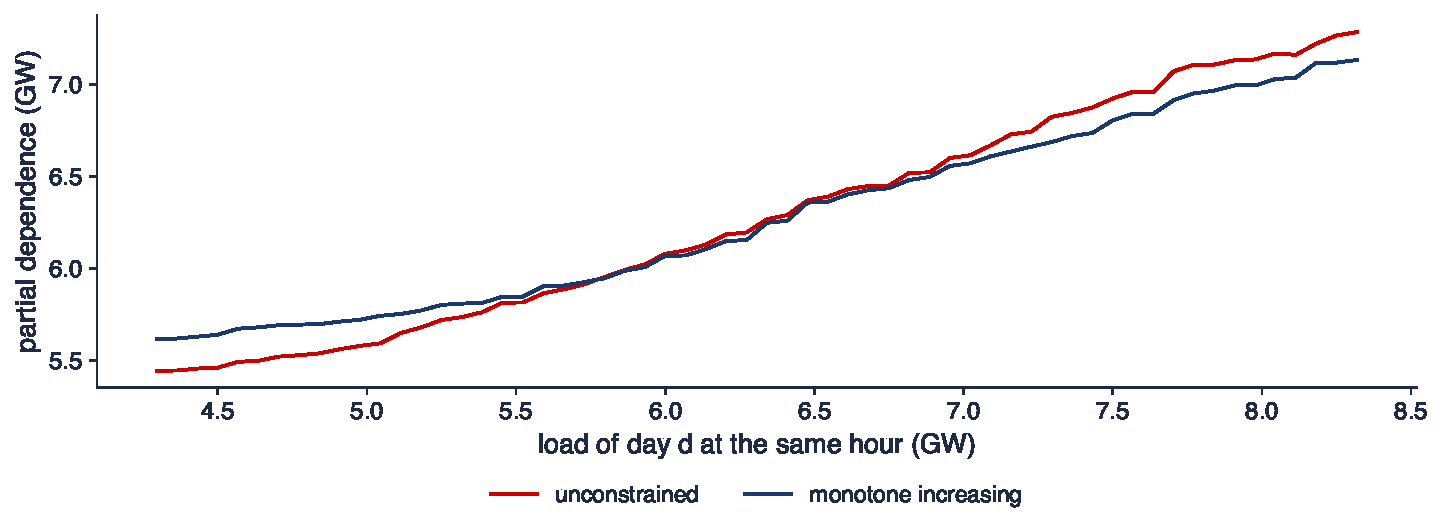
\includegraphics[width=0.97\textwidth,height=0.46\textheight,keepaspectratio]{ats_ch12_monotone.pdf}
\end{center}
\vspace{-0.25cm}
\begin{itemize}
    \item Dependența parțială a prognozei boosting de consumul din ziua $d$ la aceeași oră, antrenat pe 2023--2024
\end{itemize}
\quantlet{ATS\_ch12\_trees}{\qlurl{ATS_ch12_trees}}
\end{frame}

\begin{frame}{Interpretarea restricției}
\itemsize{\small}
\begin{itemize}
    \item Fără restricție: 3 pași descrescători (cel mai mare de 7{,}5 MW): mai mult consum ieri ar însemna uneori mai puțin consum mîine, o potrivire a zgomotului
    \item Cu restricție: monoton prin construcție; amplitudinea totală 1{,}52 GW față de 1{,}84 GW: o parte a efectului trece la celelalte laguri
    \item Acuratețea abia se schimbă (228 față de 225 MW); cîștigul este plauzibilitatea și robustețea la marginile datelor
    \item Restricțiile sînt calea prin care cunoașterea economică intră într-o cutie neagră: restricții de semn, ca în \atschlink{https://danpele.github.io/Advanced-Time-Series/RO/Cursuri/capitol3_modele_var_structurale_proiectii_locale.pdf}{Capitolul 3}, dar pentru algoritmi neliniari
\end{itemize}
\end{frame}

\begin{frame}{Recapitulare: ansamblurile de arbori}
\itemsize{\small}
\begin{itemize}
    \item Bagging-ul și pădurile reduc varianța pînă la pragul $\rho\sigma^2$; decorelarea, nu numărul de arbori, îl coboară
    \item QRF dă întreaga distribuție condiționată dintr-o singură pădure; boosting-ul ajustează gradienți, cu frunze de ordinul doi și histograme în LightGBM
    \item Pe consumul României, arborii egalează ARX-ul expert, dar nu îl depășesc; combinația lor cîștigă
\end{itemize}
\end{frame}


%=============================================================================
\section{Deep learning pentru secvențe}
%=============================================================================

\begin{frame}{De la MLP la modelele de secvențe}
\itemsize{\small}
\begin{columns}[T]
\begin{column}{0.32\textwidth}
\centering
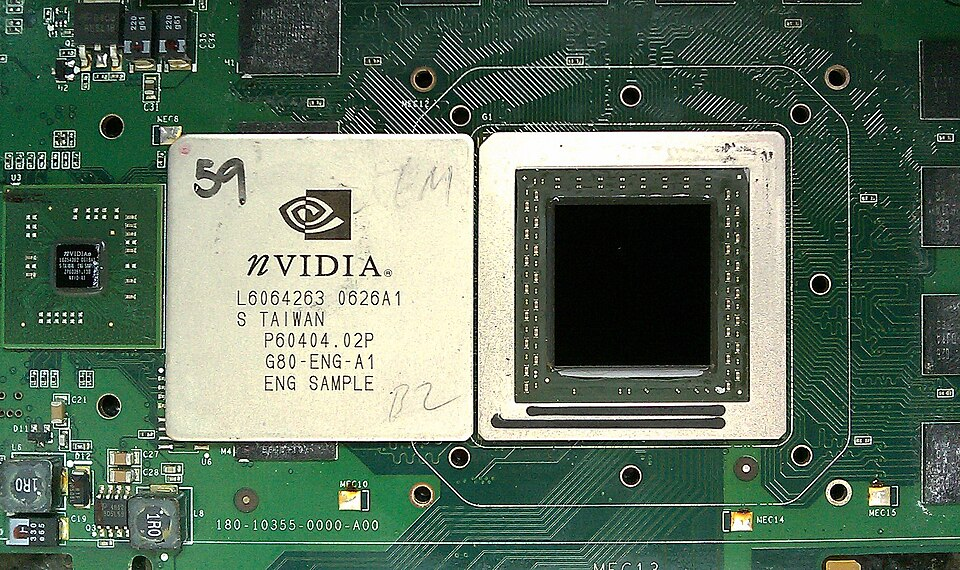
\includegraphics[height=0.3\textheight]{ch12_nvidia_g80.jpg}\\[1mm]
\imgcap{NVIDIA G80, primul procesor grafic CUDA (2006)}
\imgcredit{https://commons.wikimedia.org/wiki/File:NVIDIA_G80_GPU_Core.jpg}{Foto: Hyins (2011); domeniu public; Wikimedia Commons}
\end{column}
\begin{column}{0.66\textwidth}
\begin{itemize}
    \item Un MLP pe o fereastră de $L$ laguri este un AR($L$) neliniar
    \[ \hat y_{t+h} = W_2\,\sigma(W_1x_t + b_1) + b_2 \]
    \begin{itemize}
        \item $x_t$: cele mai recente $L$ valori; $W_1$, $W_2$: matricele de ponderi; $b_1$, $b_2$: termenii liberi (bias); $\sigma$: funcția de activare aplicată pe elemente (ReLU sau tanh)
    \end{itemize}
    \item Antrenarea: retropropagare \refRHW\ cu Adam \refKB; oprire timpurie pe ultimul bloc al eșantionului de antrenare; intrări standardizate doar cu momentele de antrenare
    \item Aproximarea universală nu spune nimic despre necesarul de date: cu cîteva mii de observații zilnice, o rețea are puțin spațiu față de un model liniar
    \item Modelele de secvențe partajează ponderile în timp: recurență (RNN), convoluție (TCN) sau atenție (Transformer)
\end{itemize}
\end{column}
\end{columns}
\end{frame}

\begin{frame}{Rețele recurente și retropropagarea în timp (1/2)}
\itemsize{\small}
\begin{itemize}
    \item RNN Elman: o stare ascunsă actualizată cu aceleași ponderi la fiecare pas
    \[ h_t = \tanh(W h_{t-1} + U x_t + b), \qquad \hat y_t = V h_t \]
    \begin{itemize}
        \item $h_t$: starea ascunsă, un rezumat învățat al trecutului (ca starea Kalman din \atschlink{https://danpele.github.io/Advanced-Time-Series/RO/Cursuri/capitol6_modele_spatiul_starilor_filtrare_bayesiana.pdf}{Capitolul 6}); $x_t$: intrarea; $W$, $U$, $V$, $b$: ponderi comune tuturor momentelor
    \end{itemize}
    \item Retropropagarea în timp (BPTT): gradientul însumează contribuțiile tuturor pașilor trecuți
    \[ \frac{\partial\mathcal L_T}{\partial W} = \sum_{t\le T}\frac{\partial\mathcal L_T}{\partial h_T}\Big(\prod_{k=t+1}^T\frac{\partial h_k}{\partial h_{k-1}}\Big)\frac{\partial^+ h_t}{\partial W} \]
    \[ \frac{\partial h_k}{\partial h_{k-1}} = \mathrm{diag}(1 - h_k^2)\,W \]
    \begin{itemize}
        \item $\mathcal L_T$: pierderea la momentul $T$; $\partial^+h_t/\partial W$: efectul direct al lui $W$ la pasul $t$; contribuția lagului $T - t$ este un produs de $T - t$ jacobiene
    \end{itemize}
\end{itemize}
\end{frame}

\begin{frame}{Rețele recurente și retropropagarea în timp (2/2)}
\itemsize{\small}
\begin{itemize}
    \item \refBSF, \refPMB: produsul jacobienelor este mărginit geometric
    \[ \Big\|\prod_{k=t+1}^T\frac{\partial h_k}{\partial h_{k-1}}\Big\| \le (\gamma\,\|W\|)^{T-t}, \qquad \gamma = \max|\tanh'| \le 1 \]
    \begin{itemize}
        \item $\gamma\|W\| < 1$: gradienți care \textbf{se sting}, lagurile lungi nu pot fi învățate
        \item raza spectrală a lui $W$ peste 1: posibilă \textbf{explozie}, tratată prin limitarea normei gradientului
    \end{itemize}
\end{itemize}
\end{frame}

\begin{frame}{LSTM și GRU: porțile (1/2)}
\itemsize{\footnotesize}
\begin{columns}[T]
\begin{column}{0.28\textwidth}
\centering

\includegraphics[height=0.36\textheight]{ch12_hochreiter_2015.jpg}\\[1mm]
\imgcap{Sepp Hochreiter, coautor al LSTM}
\imgcredit{https://commons.wikimedia.org/wiki/File:Sepp_Hochreiter.JPG}{Foto: Eulenreich (2015); CC BY-SA 4.0; Wikimedia Commons}
\end{column}
\begin{column}{0.7\textwidth}
\begin{itemize}
    \item LSTM \refHS: trei porți și un candidat, toate calculate din $[h_{t-1}, x_t]$
    \[ i_t, f_t, o_t = \sigma(W_\bullet[h_{t-1}, x_t] + b_\bullet) \]
    \[ \tilde c_t = \tanh(W_c[h_{t-1}, x_t] + b_c) \]
    \begin{itemize}
        \item $i_t$: poarta de intrare; $f_t$: poarta de uitare; $o_t$: poarta de ieșire; $\sigma$: funcția logistică, cu valori în $(0, 1)$; $\tilde c_t$: memoria candidată
    \end{itemize}
    \item Celula și ieșirea
    \[ c_t = f_t\odot c_{t-1} + i_t\odot\tilde c_t, \qquad h_t = o_t\odot\tanh(c_t) \]
    \begin{itemize}
        \item $\odot$: produsul pe elemente; de-a lungul celulei $\partial c_t/\partial c_{t-1} = \mathrm{diag}(f_t)$: aditiv, fără compresie
    \end{itemize}
\end{itemize}
\end{column}
\end{columns}
\end{frame}

\begin{frame}{LSTM și GRU: porțile (2/2)}
\itemsize{\small}
\begin{itemize}
    \item Poarta de uitare \refGSC\ trebuie să rămînă deschisă: $f \approx 1$
    \begin{itemize}
        \item un bias de 1 al porții de uitare este inițializarea obișnuită \refJZS: $\sigma(1) = 0{,}73$ la începutul antrenării
    \end{itemize}
    \item GRU \refCho: două porți, de actualizare $z_t$ și de resetare $r_t$
    \[ h_t = (1 - z_t)\odot h_{t-1} + z_t\odot\tilde h_t \]
    \begin{itemize}
        \item $\tilde h_t$: starea candidată, calculată din $r_t\odot h_{t-1}$ și $x_t$; mai puțini parametri decît LSTM, comportament asemănător
    \end{itemize}
\end{itemize}
\end{frame}

\begin{frame}{Distanța în timp pînă la care ajunge gradientul}
\itemsize{\footnotesize}
\begin{center}
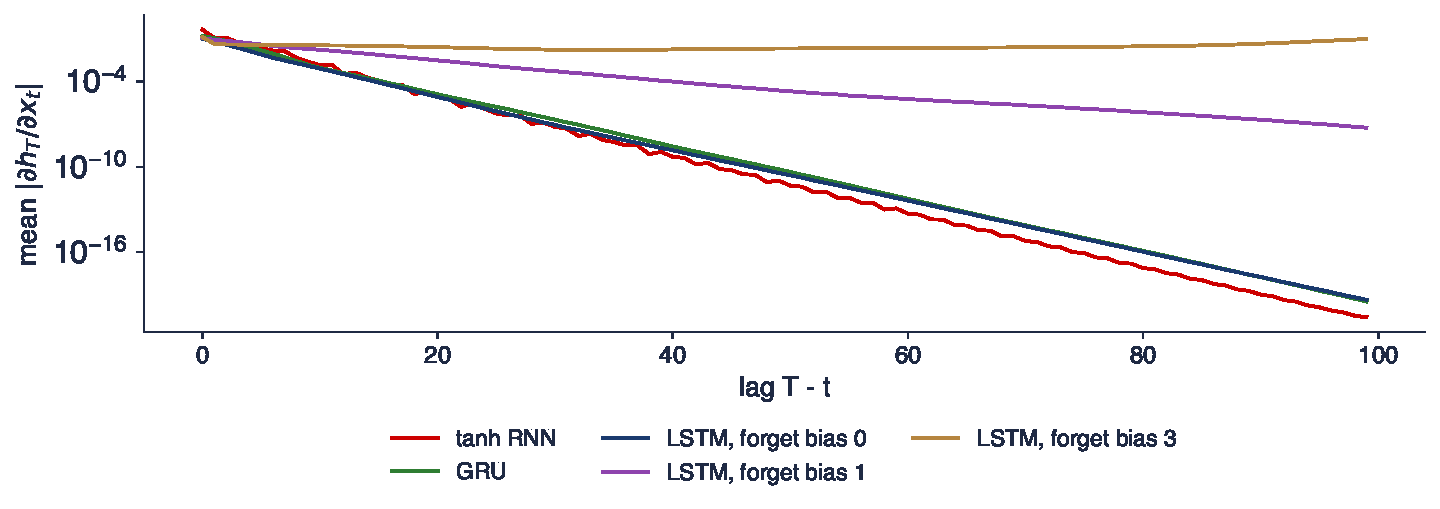
\includegraphics[width=0.97\textwidth,height=0.5\textheight,keepaspectratio]{ats_ch12_vanishing.pdf}
\end{center}
\vspace{-0.25cm}
\begin{itemize}
    \item Media $|\partial h_T/\partial x_t|$ pentru rețele proaspăt inițializate (32 de unități, $T = 100$, intrări gaussiene, media a 5 seed-uri), scară logaritmică
\end{itemize}
\quantlet{ATS\_ch12\_recurrent}{\qlurl{ATS_ch12_recurrent}}
\end{frame}

\begin{frame}{Interpretarea gradienților}
\itemsize{\small}
\begin{itemize}
    \item La lagul 50, gradientul este o fracțiune $10^{-10}$ din valoarea de la lagul 1 pentru RNN tanh, $10^{-9}$ pentru GRU și $10^{-9}$ pentru LSTM cu bias-ul implicit 0 al porții de uitare
    \item Bias 1 al porții de uitare: $10^{-4}$; bias 3: 0{,}47: porțile ajută doar cînd poarta de uitare este deschisă ($\sigma(3) = 0{,}95$)
    \item Ratele de stingere pe lag: 0{,}51 (RNN), 0{,}45 (LSTM, bias 0), 0{,}03 (LSTM, bias 3): geometrice în toate cazurile
    \item Pentru seriile zilnice contează mai puțin decît pare: memoria de tip HAR (22 de laguri) este accesibilă; pentru datele orare cu ciclu săptămînal (168 de laguri), ea decide arhitectura
\end{itemize}
\end{frame}

\begin{frame}{Rețele convoluționale temporale}
\itemsize{\small}
\begin{itemize}
    \item Convoluția cauzală dilatată: o sumă ponderată a intrărilor trecute, aflate la distanță de $d$ pași \refWaveNet
    \[ z_t = \sum_{j=0}^{k-1} w_j\,x_{t - d\,j} \]
    \begin{itemize}
        \item $k$: mărimea nucleului; $w_j$: ponderile filtrului; $d$: dilatarea (sare $d - 1$ pași); intră doar trecutul (cauzal)
        \item TCN \refBaiK: blocuri reziduale cu cîte două convoluții cauzale dilatate, $d = 1, 2, 4, \dots, 2^{\ell-1}$ pe $\ell$ niveluri
    \end{itemize}
    \item Cîmpul receptiv: cît de departe în trecut poate privi rețeaua
    \[ R = 1 + 2(k - 1)(2^\ell - 1) \]
    \begin{itemize}
        \item $k = 3$, $\ell = 4$: $R = 61$; o săptămînă de ore cere $\ell = 7$ ($R = 509$); memoria este fixată de arhitectură: fără stingere în timp, dar nimic dincolo de $R$
    \end{itemize}
    \item Paralelă în timp (antrenare rapidă), gradienți stabili; Bai et al.\ au găsit TCN competitive cu LSTM pe sarcini standard de secvențe
\end{itemize}
\end{frame}

\begin{frame}{Prognoze pe mai mulți pași și sequence-to-sequence}
\itemsize{\small}
\begin{itemize}
    \item \textbf{Recursiv}: un model la un pas iterat, prognozele reintroduse ca intrări: erorile se acumulează, modelul este antrenat doar pentru $h = 1$
    \item \textbf{Direct}: un model pentru fiecare orizont $h$ (prognozele HAR și ale rețelelor de aici); \textbf{MIMO}: o rețea dă întregul vector $(\hat y_{t+1},\dots,\hat y_{t+H})$ (DLinear, N-BEATS, Transformers aici)
    \item \textbf{Encoder--decoder} \refSVL: o rețea recurentă codifică trecutul într-o stare, alta desfășoară viitorul; antrenare cu teacher forcing
    \begin{itemize}
        \item deplasarea de expunere: la test, decodorul își vede propriile erori; DeepAR simulează în schimb traiectorii
    \end{itemize}
    \item Sinteza practicii recurente \refHBB: desezonalizare sau laguri sezoniere, scalare pe serie, antrenare globală, ansamblu de seed-uri
\end{itemize}
\end{frame}

\begin{frame}{Schema studiului: modele deep față de HAR}
\itemsize{\small}
\begin{itemize}
    \item Ținta $y = \log RV$ pentru S\&P 500 (\refOMI); prognoze ale $RV_{t+h}$, $h \in \{1, 5, 22\}$, directe; prognoza nivelului $\exp(\hat m + s^2/2)$ cu varianța reziduală de antrenare
    \item Fereastră extinsă, prima prognoză după 2500 de zile (24 decembrie 2009), reestimare la fiecare 500 de zile; 3\,051 de prognoze pe orizont
    \item Modele pe ultimele 22 de valori: HAR \refCor\ (OLS), MLP (2 $\times$ 32 de unități), LSTM (16 unități), TCN (3 niveluri, $R = 29$), HGB pe cele 22 de laguri; un seed pe rețea
    \item QLIKE \refPat, DM (HLN) față de HAR, MCS; literatura: rețelele neuronale cîștigă puțin față de HAR \refBuc; cîștigurile ML apar mai ales cu mulți predictori \refCSV
\end{itemize}
\end{frame}

\begin{frame}{Rețele deep față de HAR}
\itemsize{\footnotesize}
\begin{center}
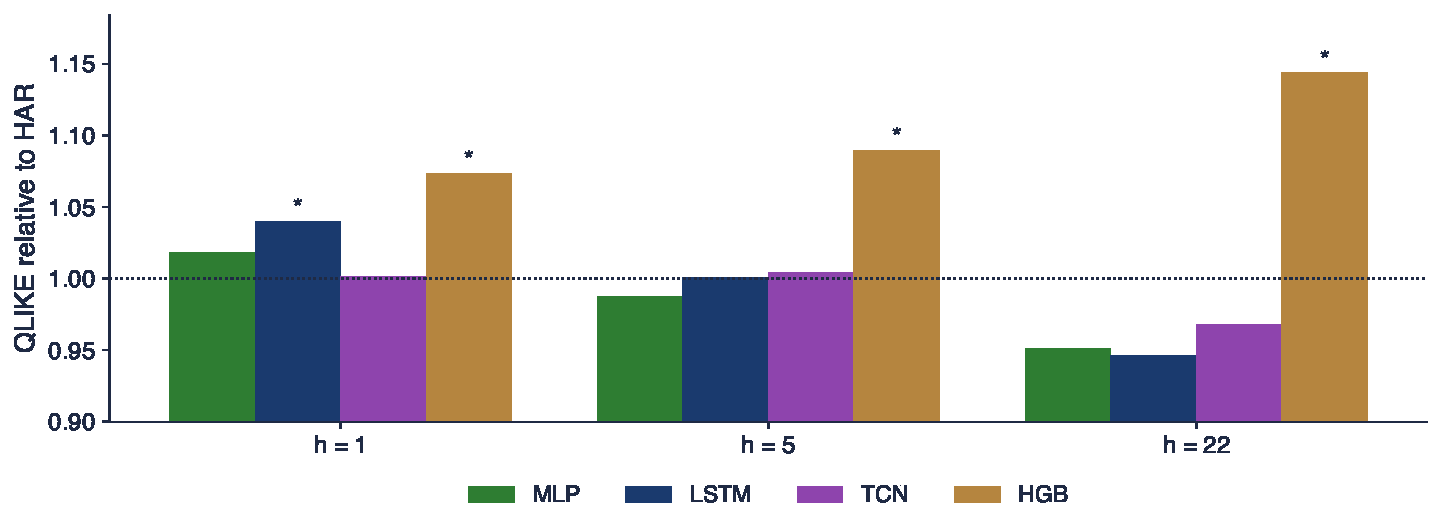
\includegraphics[width=0.97\textwidth,height=0.5\textheight,keepaspectratio]{ats_ch12_rv_deep.pdf}
\end{center}
\vspace{-0.25cm}
\begin{itemize}
    \item QLIKE relativ la HAR (1 = HAR); steaua marchează o respingere DM la 5\%
\end{itemize}
\quantlet{ATS\_ch12\_recurrent}{\qlurl{ATS_ch12_recurrent}}
\end{frame}

\begin{frame}{Interpretarea modelelor deep față de HAR}
\itemsize{\small}
\begin{itemize}
    \item $h = 1$: MLP 1{,}019, LSTM 1{,}040 (DM 2{,}77), TCN 1{,}002, HGB 1{,}074 (DM 3{,}84): niciun model nu este mai bun decît HAR, două modele sînt semnificativ mai slabe
    \item $h = 22$: MLP 0{,}951, LSTM 0{,}946, TCN 0{,}968: cîștiguri de 3--5\% pe care DM nu le confirmă ($p$ 0{,}132; 0{,}444); HAR rămîne în MCS ($p$ 0{,}49)
    \item Boosting-ul pe lagurile brute este cel mai slab la toate orizonturile: arborii nu pot extrapola la vîrfurile de volatilitate din 2020
    \item HAR este un model liniar cu cele trei variabile potrivite; o rețea trebuie să le redescopere din cîteva mii de zile
\end{itemize}
\end{frame}

\begin{frame}{Recapitulare: deep learning pentru secvențe}
\itemsize{\small}
\begin{itemize}
    \item Gradienții în timp sînt produse de jacobiene: se sting geometric, cu excepția cazului în care poarta de uitare LSTM rămîne deschisă
    \item TCN fixează memoria prin cîmpul receptiv; prognozele pe mai mulți pași sînt recursive, directe sau MIMO
    \item Pe varianța realizată zilnică, rețelele nu sînt semnificativ mai bune decît HAR la niciun orizont
\end{itemize}
\end{frame}


%=============================================================================
\section{Atenție și Transformers}
%=============================================================================

\begin{frame}{Atenția cu produs scalar scalat}
\itemsize{\small}
\begin{itemize}
    \item \refVas: fiecare token „privește” toți tokenii, cu ponderi date de similaritatea interogare--cheie
    \[ Q = XW_Q, \quad K = XW_K, \quad V = XW_V \]
    \[ \mathrm{Att}(Q, K, V) = \mathrm{softmax}\Big(\frac{QK'}{\sqrt{d_k}}\Big)V \]
    \begin{itemize}
        \item $X \in \mathbb R^{n\times d}$: $n$ tokeni de dimensiune $d$; $W_Q, W_K, W_V$: proiecții învățate în interogări, chei și valori; $d_k$: dimensiunea cheilor; softmax normalizează fiecare rînd în ponderi care însumează 1
        \item fiecare ieșire este o medie ponderată a valorilor, cu ponderi dependente de date; $\sqrt{d_k}$ menține logiții de ordinul unu; multi-head: mai multe proiecții în paralel, concatenate
    \end{itemize}
    \item Echivariantă la permutări: fără \textbf{codificări poziționale}, ordinea tokenilor se pierde, ceea ce este fatal pentru serii de timp
    \item Cost $O(n^2 d)$ în timp și memorie: un token pe oră și o săptămînă de intrare dau $n = 168$; o lună dă $n = 720$
    \begin{itemize}
        \item Transformers pentru orizonturi lungi din 2020--2022 au urmărit mai ales acest cost
    \end{itemize}
\end{itemize}
\end{frame}

\begin{frame}{Transformers pentru orizonturi lungi}
\itemsize{\small}
\begin{itemize}
    \item \textbf{Informer} \refInf: atenție ProbSparse (doar interogările cele mai informative), distilarea atenției, un decodor generativ care dă orizontul dintr-o dată: $O(n\log n)$
    \item \textbf{Autoformer} \refAuto: descompunerea seriei în fiecare strat (trend prin medie mobilă și rest) și un mecanism de autocorelație care agregă subserii la laguri găsite prin FFT
    \item \textbf{PatchTST} \refNie: tokenii sînt \textbf{segmente} de valori consecutive (de exemplu 16 sau 24), fiecare canal modelat separat, normalizare pe instanță
    \begin{itemize}
        \item mai puțini tokeni ($n/P$), semnificație locală în fiecare token, ferestre de intrare mai lungi accesibile
    \end{itemize}
    \item Toate au fost evaluate pe aceleași cîteva seturi de date (electricitate, trafic, vreme, ETT), cu MSE pe date standardizate
\end{itemize}
\end{frame}

\begin{frame}{Critica lui Zeng et al.\ (2023): eficiența Transformers}
\itemsize{\small}
\begin{itemize}
    \item \refZeng: auto-atenția este invariantă la permutări; tokenii punctuali nu au semnificație locală; codificările poziționale restabilesc ordinea doar parțial
    \item Reperele LTSF-Linear: o singură aplicație liniară de la ultimele $L$ valori la următoarele $H$
    \[ \textbf{Linear:}\ \hat y_{t+1:t+H} = W\,x_{t-L+1:t} \]
    \[ \textbf{DLinear:}\ \hat y = \big(W_s(I - A) + W_tA\big)\,x \]
    \begin{itemize}
        \item $W$: o matrice de ponderi $H \times L$; \textbf{NLinear} scade și adaugă înapoi ultima valoare; \textbf{DLinear}: $A$ matricea mediei mobile, $W_t$ pentru trendul $Ax$, $W_s$ pentru rest (Seminarul 12, A8)
    \end{itemize}
    \item Rezultatul lor: aceste modele cu un singur strat sînt mai bune decît Informer, Autoformer și succesorii lor pe majoritatea seturilor standard pentru orizonturi lungi
    \begin{itemize}
        \item iar Transformers nu se îmbunătățeau cu o fereastră $L$ mai lungă: un semn că nu foloseau istoria suplimentară
    \end{itemize}
    \item PatchTST a fost răspunsul: segmentarea și independența canalelor au readus Transformers înaintea DLinear pe aceleași seturi de date
\end{itemize}
\end{frame}

\begin{frame}{Schema replicării: protocolul Zeng et al.\ pe consumul României}
\itemsize{\small}
\begin{itemize}
    \item Consumul orar al României ca o singură serie ($n = 32\,856$ ore), standardizat cu momentele de antrenare; împărțire cronologică 7:1:2; testul de la 31 decembrie 2025
    \item Fereastra de intrare $L = 336$ de ore; orizonturi $H = 96$ și $336$; MSE și MAE pe seria standardizată, ca în tabelele lor
    \item Modele: repetarea ultimei valori, naiv sezonier (ultima săptămînă), Linear, NLinear, DLinear (nucleu 25), un Transformer pe segmente (14 segmente de 24 de ore, 1 strat, 4 capete) și același Transformer cu un token pe oră
    \item Adam, MSE, oprire timpurie pe blocul de validare; media a trei seed-uri (unul pentru Transformer-ul cu tokeni punctuali, al cărui cost este $O(n^2)$)
\end{itemize}
\end{frame}

\begin{frame}{Modele liniare, Transformers și rolul tokenilor}
\itemsize{\footnotesize}
\begin{center}
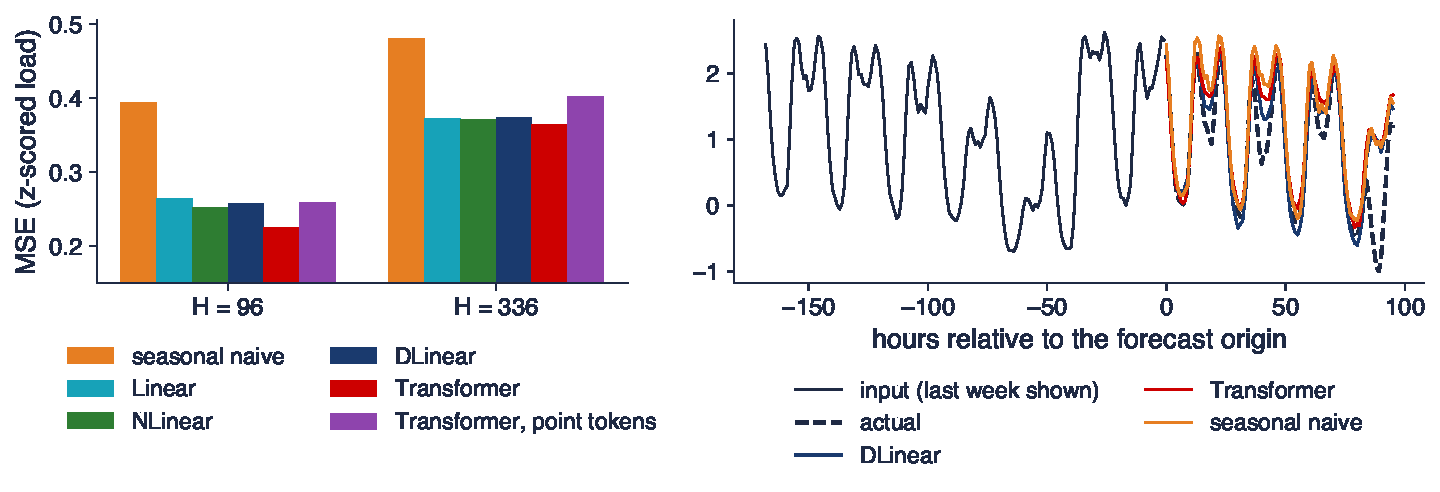
\includegraphics[width=0.97\textwidth,height=0.48\textheight,keepaspectratio]{ats_ch12_zeng.pdf}
\end{center}
\vspace{-0.25cm}
\begin{itemize}
    \item Stînga: MSE de test după orizont (repetarea ultimei valori, 1{,}585 și 1{,}699, iese din scară); dreapta: o fereastră de test la $H = 96$ (ultima săptămînă de intrare, consumul real și trei prognoze)
\end{itemize}
\quantlet{ATS\_ch12\_transformers}{\qlurl{ATS_ch12_transformers}}
\end{frame}

\begin{frame}{Interpretarea protocolului}
\itemsize{\small}
\begin{itemize}
    \item $H = 96$: naiv sezonier 0{,}393, Linear 0{,}265, NLinear 0{,}253, DLinear 0{,}257; Transformer cu tokeni punctuali 0{,}258; Transformer pe segmente 0{,}226
    \item $H = 336$: DLinear 0{,}374, tokeni punctuali 0{,}402 (mai slab decît orice model liniar), segmente 0{,}364
    \item Ambele lucrări se replică pe datele noastre: Transformer-ul cu tokeni punctuali nu este mai bun decît NLinear sau DLinear la $H = 96$ și este mai slab decît orice model liniar la $H = 336$; segmentarea răstoarnă clasamentul
    \item Distanța dintre cel mai bun model liniar și Transformer-ul pe segmente scade de la 0{,}253 față de 0{,}226 la $H = 96$ la 0{,}371 față de 0{,}364 la $H = 336$: la orizonturi lungi seria este mai ales nivel sezonier
\end{itemize}
\end{frame}

\begin{frame}{Temporal Fusion Transformer}
\itemsize{\small}
\begin{itemize}
    \item \refTFT: construit pentru prognoze pe mai multe orizonturi, cu trei tipuri de intrări: statice (magazinul, țara), viitoare cunoscute (calendar, prețuri), trecute observate
    \item Componente
    \begin{itemize}
        \item rețele reziduale cu poartă (GRN): $\mathrm{LayerNorm}\big(a + \mathrm{GLU}(\eta)\big)$, o poartă care poate opri un bloc
        \item rețele de selecție a variabilelor: ponderi softmax pe intrări la fiecare moment
        \item codificatori ai covariatelor statice care condiționează celelalte blocuri; un encoder--decoder LSTM pentru tipare locale
        \item atenție multi-head interpretabilă (valori comune tuturor capetelor) pentru dependența de lungă durată; ieșiri cuantilice antrenate cu pierderea pinball
    \end{itemize}
    \item „Interpretabilitatea” lui înseamnă ponderile de selecție a variabilelor și tiparul atenției: diagnostice utile, nu explicații cauzale (secțiunea 7)
\end{itemize}
\end{frame}

\begin{frame}{Recapitulare: atenție și Transformers}
\itemsize{\small}
\begin{itemize}
    \item Atenția este o medie ponderată dependentă de date; ordinea vine doar din codificările poziționale; costul este pătratic în numărul de tokeni
    \item Zeng et al.: un strat liniar a fost mai bun decît Transformers cu tokeni punctuali; PatchTST: segmentele refac avantajul; ambele se replică pe consumul României
    \item TFT organizează intrările statice, cunoscute și observate prin porți, selecție și atenție și dă cuantile
\end{itemize}
\end{frame}


%=============================================================================
\section{Modele deep globale: N-BEATS, N-HiTS, DeepAR}
%=============================================================================

\begin{frame}{N-BEATS: dezvoltare în baze de funcții cu stivuire reziduală}
\itemsize{\small}
\begin{itemize}
    \item \refOre: fiecare bloc reconstruiește o parte a intrării (backcast) și prognozează restul
    \[ \hat x_\ell = g^b(\theta^b_\ell), \quad \hat y_\ell = g^f(\theta^f_\ell) \]
    \[ x_{\ell+1} = x_\ell - \hat x_\ell, \quad \hat y = \sum_\ell\hat y_\ell \]
    \begin{itemize}
        \item $x_\ell$: intrarea blocului $\ell$; $\theta^b_\ell, \theta^f_\ell$: coeficienții produși de patru straturi complet conectate; $g^b$, $g^f$: funcțiile de bază; dublu rezidual: fiecare bloc explică ce au lăsat cele anterioare
    \end{itemize}
    \item \textbf{Generic}: $g$ liniar și învățat; \textbf{interpretabil}: baza de trend $\{(t/H)^j\}_{j\le3}$ și baza sezonieră $\{\cos 2\pi jt/H, \sin 2\pi jt/H\}$
    \begin{itemize}
        \item $H$: orizontul prognozei; o descompunere învățată, asemănătoare netezirii exponențiale
    \end{itemize}
    \item Deep learning pur, fără variabile specifice seriilor de timp; antrenat global pe fiecare frecvență cu pierderi sMAPE/MASE; rezultatele publicate sînt ansambluri de 180 de rețele
    \begin{itemize}
        \item rezultatul lor pe M4 l-a depășit pe cîștigătorul competiției, hibridul ES-RNN al lui \refSmyl
    \end{itemize}
\end{itemize}
\end{frame}

\begin{frame}{N-HiTS: intrări pe mai multe rate, ieșiri ierarhice}
\itemsize{\small}
\begin{itemize}
    \item \refNHiTS: blocul $\ell$ aplică întîi max-pooling cu nucleul $k_\ell$ (de exemplu 8, 4, 1): blocurile de rezoluție mică văd forma pe termen lung, cele de rezoluție mare detaliul
    \item Fiecare bloc dă doar $H/r_\ell$ coeficienți, interpolați la $H$ puncte: raportul de expresivitate $r_\ell$ obligă blocurile grosiere să prognozeze componente netede
    \begin{itemize}
        \item o descompunere explicită pe frecvențe a prognozei, apropiată de multirezoluția wavelet din \atschlink{https://danpele.github.io/Advanced-Time-Series/RO/Cursuri/capitol11_analiza_spectrala_analiza_wavelet.pdf}{Capitolul 11}
    \end{itemize}
    \item Mai puțini parametri și mai puțin calcul decît N-BEATS la orizonturi lungi, cu acuratețe asemănătoare la cele scurte
    \item Ale noastre: N-BEATS generic (3 blocuri $\times$ 3 straturi $\times$ 256 de unități) și N-HiTS (pooling 8, 4, 1), intrare de 336 de ore, fiecare fereastră împărțită la nivelul ei mediu absolut, pierdere MAE, mediana a 3 seed-uri
\end{itemize}
\end{frame}

\begin{frame}{Schema studiului: subsetul orar M4}
\itemsize{\small}
\begin{itemize}
    \item \refMfourA: 414 de serii orare, orizont 48
    \item Măsurile de acuratețe: MAPE simetric, eroarea scalată și media lor relativă la Naive 2
    \[ \mathrm{OWA} = \frac12\Big(\frac{\mathrm{sMAPE}}{\mathrm{sMAPE}_{\mathrm{Naive2}}} + \frac{\mathrm{MASE}}{\mathrm{MASE}_{\mathrm{Naive2}}}\Big) \]
    \begin{itemize}
        \item sMAPE: media lui $2|y - \hat y|/(|y| + |\hat y|)$, în \%; MASE: eroarea absolută medie împărțită la MAE din eșantion al naivului sezonier (perioada 24) \refHK; OWA $< 1$: mai bun decît Naive 2
    \end{itemize}
    \item Naive, naivul sezonier și Naive 2 calculate aici reproduc exact fișierul oficial de evaluare M4: Naive 2 sMAPE 18{,}38 (oficial 18{,}38), MASE 2{,}40 (oficial 2{,}40)
    \item Repere din același fișier: reperele M4 MLP și RNN (OWA 0{,}921 și 1{,}036), Theta 1{,}006, cîștigătorul \refSmyl\ 0{,}440, locul doi Montero-Manso et al.\ 0{,}484; toate modelele globale sînt antrenate doar pe părțile de antrenare
\end{itemize}
\end{frame}

\begin{frame}{Modele deep globale pe seriile orare M4}
\itemsize{\footnotesize}
\begin{center}
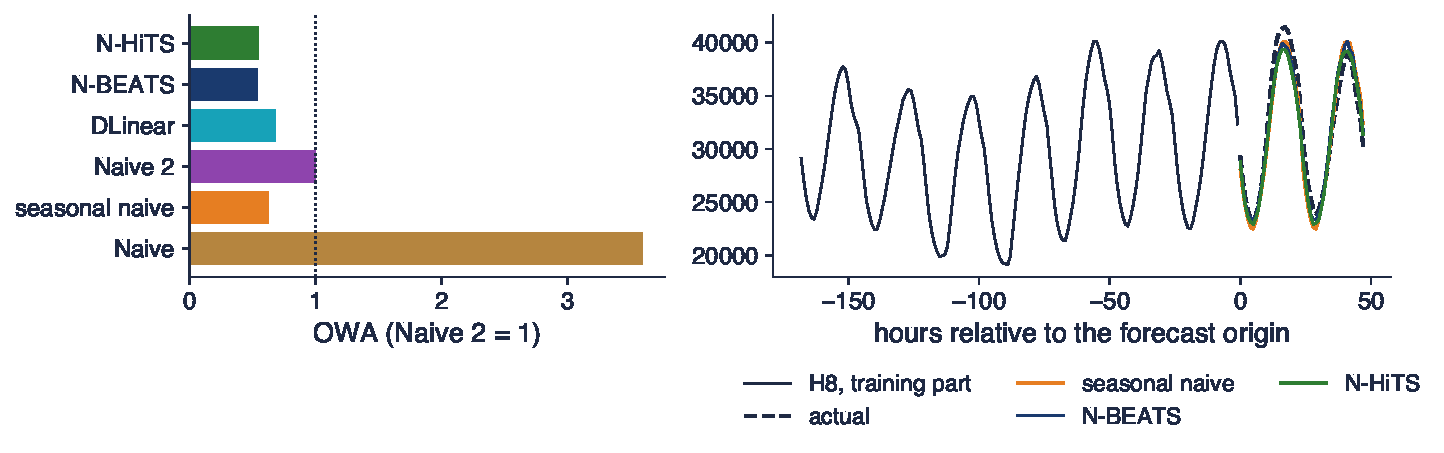
\includegraphics[width=0.97\textwidth,height=0.48\textheight,keepaspectratio]{ats_ch12_m4.pdf}
\end{center}
\vspace{-0.25cm}
\begin{itemize}
    \item Stînga: OWA (Naive 2 = 1); dreapta: o serie cu prognozele naivului sezonier, N-BEATS și N-HiTS
\end{itemize}
\quantlet{ATS\_ch12\_global\_deep}{\qlurl{ATS_ch12_global_deep}}
\end{frame}

\begin{frame}{Interpretarea rezultatelor M4 orare}
\itemsize{\small}
\begin{itemize}
    \item OWA: naiv sezonier 0{,}628, DLinear 0{,}683, N-BEATS 0{,}539 (sMAPE 10{,}73, MASE 1{,}19), N-HiTS 0{,}548
    \item Cîteva minute de antrenare pe procesor pun N-BEATS înaintea tuturor reperelor M4 și a reperelor neuronale M4 (0{,}921; 1{,}036), în urma primelor două participări (0{,}440; 0{,}484)
    \item Reperele neuronale M4 erau locale (o rețea pe serie); ale noastre sînt globale: reunirea celor 414 serii face diferența
    \item DLinear este mai slab aici: seriile orare M4 cer interacțiuni neliniare între nivel și sezon pe care un singur strat liniar nu le poate exprima
\end{itemize}
\end{frame}

\begin{frame}{DeepAR: prognoze probabilistice dintr-o rețea recurentă globală}
\itemsize{\small}
\begin{itemize}
    \item \refDeepAR: o stare LSTM pentru fiecare serie determină parametrii unei verosimilități
    \[ h_{i,t} = \mathrm{LSTM}(h_{i,t-1}, z_{i,t-1}, x_{i,t}), \qquad z_{i,t} \sim \ell\big(\cdot\mid\theta(h_{i,t})\big) \]
    \begin{itemize}
        \item $z_{i,t}$: valoarea seriei $i$ la $t$; $x_{i,t}$: covariabilele (laguri la 1, 24, 168, calendar); $\theta(h)$: de exemplu gaussiană $(\mu, \sigma)$ pentru date reale, binomială negativă pentru numărări
        \item antrenarea: maximizăm $\sum_{i,t}\log\ell(z_{i,t}\mid\theta(h_{i,t}))$ pe ferestre aleatoare din toate seriile, fiecare scalată cu $1 + $ media contextului
    \end{itemize}
    \item Prognoza: simulare ancestrală, fiecare extragere reintrodusă ca intrare următoare; cuantilele din traiectoriile simulate
    \[ \mathrm{wQL} = \sum_\tau\frac{2\sum_{i,t}\rho_\tau(z_{i,t} - \hat q_{\tau,i,t})}{\sum_{i,t}|z_{i,t}|} \]
    \begin{itemize}
        \item pierderea cuantilică ponderată: $\rho_\tau$ pierderea pinball la nivelul $\tau$, $\hat q_\tau$ cuantila prognozată; o aproximare a CRPS \refGR, o valoare mai mică este mai bună
    \end{itemize}
    \item Modelul preferat pentru paneluri mari din retail și energie; baza mai multor foundation models (\atschlink{https://danpele.github.io/Advanced-Time-Series/RO/Cursuri/capitol13_foundation_models_conformal.pdf}{Capitolul 13})
\end{itemize}
\end{frame}

\begin{frame}{Un DeepAR mic pe seriile orare M4}
\itemsize{\footnotesize}
\begin{center}
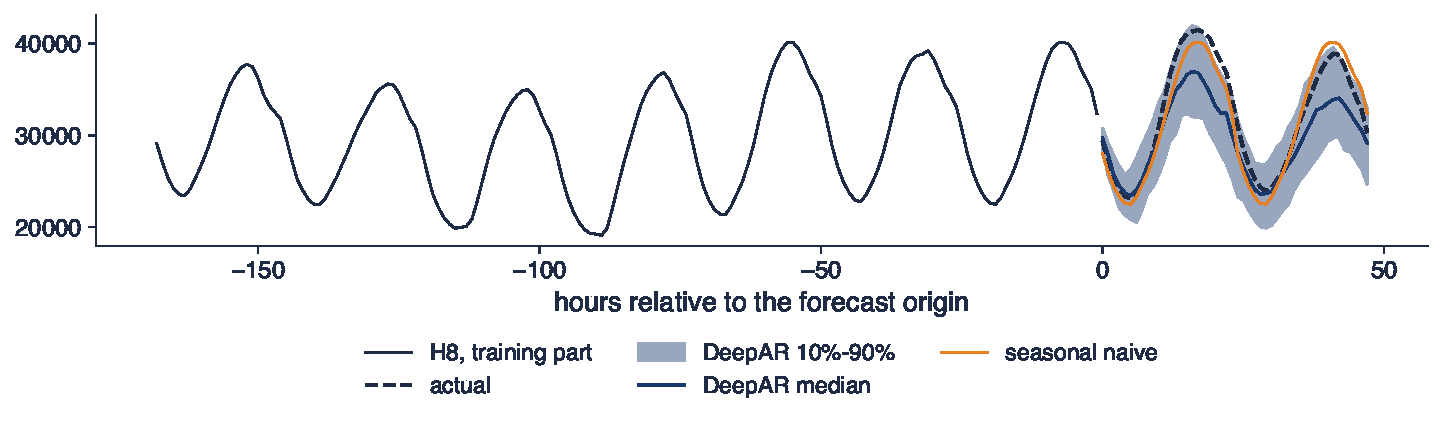
\includegraphics[width=0.97\textwidth,height=0.46\textheight,keepaspectratio]{ats_ch12_deepar.pdf}
\end{center}
\vspace{-0.25cm}
\begin{itemize}
    \item LSTM cu două straturi (40 de unități), context de 168 de ore, 4\,000 de pași de antrenare cu cîte 64 de ferestre, 100 de traiectorii simulate; aceeași serie ca în graficul anterior
\end{itemize}
\quantlet{ATS\_ch12\_global\_deep}{\qlurl{ATS_ch12_global_deep}}
\end{frame}

\begin{frame}{Interpretarea DeepAR}
\itemsize{\small}
\begin{itemize}
    \item wQL după bugetul de antrenare (pași): 500: 0{,}0344, 1000: 0{,}0338, 2000: 0{,}0374, 4000: 0{,}0405; naivul sezonier cu cuantile empirice: 0{,}0375
    \item După 1000 de pași, DeepAR este mai bun decît reperul (acoperirea de 80\%: 83\%); cu antrenare mai lungă, supraajustează ferestrele de antrenare și pierde (76\% la 4000 de pași)
    \item Alegerea celui mai bun punct de control din acest tabel ar fi data snooping: bugetul trebuie fixat pe un bloc de validare înainte de a deschide perioada de test
    \item Modelele deep probabilistice sînt sensibile la bugetul de antrenare; raportați regula care l-a fixat și reperul sub o regulă de scor proprie
\end{itemize}
\end{frame}

\begin{frame}{Lecțiile competiției M5}
\itemsize{\small}
\begin{itemize}
    \item \refMfiveA: 42\,840 de serii Walmart într-o ierarhie, vînzări zilnice în unități, 28 de zile înainte; secțiunile de acuratețe și de incertitudine
    \begin{itemize}
        \item metodele cîștigătoare la acuratețe au fost modele LightGBM globale pe variabile construite (laguri, medii mobile, prețuri, calendar), adesea combinate
    \end{itemize}
    \item Modelele globale, învățarea între serii și informația externă (prețuri, evenimente) au contat mai mult decît arhitectura
    \item Reperele simple au fost depășite, dar cu marje mai mici decît sugerează publicitatea ML și cel mai puțin la nivelul de jos al ierarhiei
    \item Un avertisment anterior: metodele ML au pierdut în fața celor statistice pe datele lunare M3 \refMSAa; diferența dintre M3 și M5 este volumul de date și învățarea între serii
\end{itemize}
\end{frame}

\begin{frame}{Recapitulare: modele deep globale}
\itemsize{\small}
\begin{itemize}
    \item N-BEATS și N-HiTS: stive reziduale de blocuri complet conectate, generice sau cu baze de trend și sezon, pe mai multe rate în N-HiTS
    \item Pe M4 orar, N-BEATS global depășește toate reperele și rețelele neuronale locale din M4
    \item DeepAR dă traiectorii dintr-o verosimilitate; depășește naivul sezonier sub wQL doar la bugetul de antrenare potrivit, care trebuie fixat pe date de validare
\end{itemize}
\end{frame}


%=============================================================================
\section{Interpretare și comparații riguroase}
%=============================================================================

\begin{frame}{Valorile Shapley (1/2): definiția}
\itemsize{\small}
\begin{itemize}
    \item \refSha: partea echitabilă a jucătorului $g$ într-un joc cooperativ $v$ cu $G$ jucători
    \[ \phi_g = \sum_{S \subseteq \{1..G\}\setminus g}\frac{|S|!\,(G - |S| - 1)!}{G!}\big[v(S\cup g) - v(S)\big] \]
    \begin{itemize}
        \item $v(S)$: valoarea coaliției $S$; $v(S\cup g) - v(S)$: contribuția marginală a lui $g$; ponderile o mediază pe toate ordinile în care jucătorii pot intra
    \end{itemize}
    \item Singura alocare care respectă patru axiome
    \begin{itemize}
        \item eficiența ($\sum_g\phi_g = v(\mathrm{toate}) - v(\emptyset)$), simetria, jucătorul nul (un jucător care nu adaugă nimic primește 0) și aditivitatea
    \end{itemize}
\end{itemize}
\end{frame}

\begin{frame}{Valorile Shapley (2/2): SHAP pentru prognoze}
\itemsize{\small}
\begin{itemize}
    \item SHAP \refLL: jucătorii sînt variabilele; valoarea unei coaliții $S$ este prognoza așteptată cînd se cunoaște doar $x_S$
    \[ v(S) = \E\big[f(x_S, X_{\bar S})\big] \]
    \begin{itemize}
        \item $f$: modelul estimat; $\bar S$: celelalte variabile; \textbf{intervențional}: $X_{\bar S}$ dintr-un eșantion de fundal, independent de $x_S$; \textbf{observațional}: condiționat de $x_S$
        \item cu laguri, variabilele sînt puternic corelate: valorile intervenționale evaluează modelul pe istorii imposibile; grupați în schimb lagurile corelate
    \end{itemize}
    \item Aici: valori Shapley exacte pentru trei grupuri de laguri (ziua, zilele 2--5, zilele 6--22) pentru boosting pe logaritmul RV S\&P 500, 300 de zile de prognoză, 100 de zile de fundal
\end{itemize}
\end{frame}

\begin{frame}{Tiparul învățat de modelul boosting}
\itemsize{\footnotesize}
\begin{center}
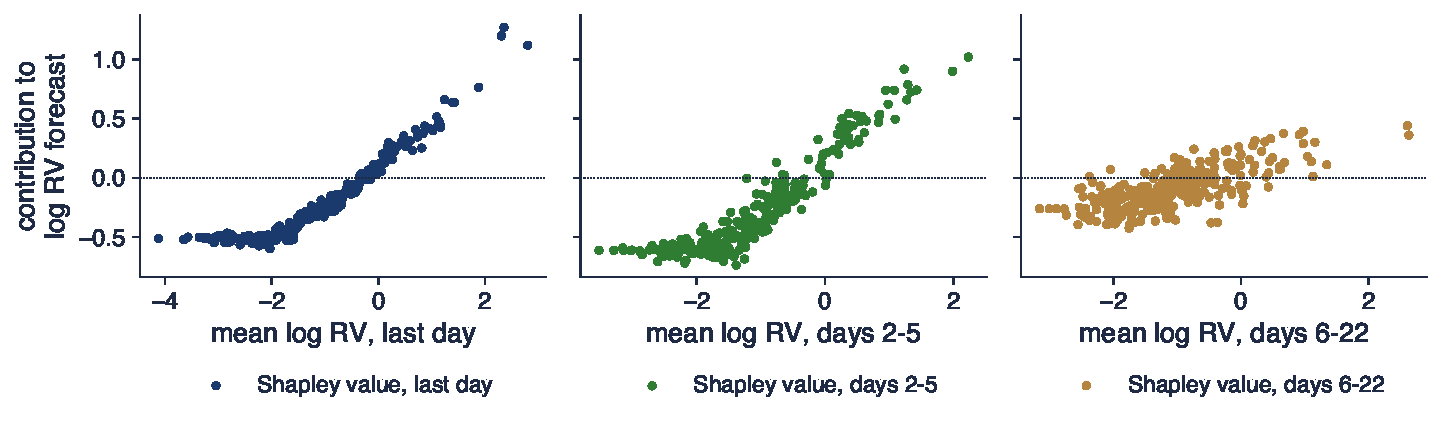
\includegraphics[width=0.97\textwidth,height=0.44\textheight,keepaspectratio]{ats_ch12_shap.pdf}
\end{center}
\vspace{-0.25cm}
\begin{itemize}
    \item Fiecare punct: o zi de prognoză; orizontal: media logaritmului RV a grupului; vertical: valoarea lui Shapley
\end{itemize}
\quantlet{ATS\_ch12\_interpretation}{\qlurl{ATS_ch12_interpretation}}
\end{frame}

\begin{frame}{Interpretarea valorilor Shapley}
\itemsize{\small}
\begin{itemize}
    \item Ponderile mediei $|\phi|$: ultima zi 37\%, zilele 2--5 46\%, zilele 6--22 17\%
    \item HAR pe același eșantion: coeficienți 0{,}28; 0{,}50; 0{,}17 pentru mediile zilnică, săptămînală și lunară: arborii boosting au redescoperit cascada HAR
    \item Valorile se aplatizează la extreme: arborii își limitează prognozele la intervalul de antrenare, motivul pentru care boosting a pierdut față de HAR în 2020
    \item Valorile Shapley descriu modelul, nu procesul generator: descrierea corectă a unui model greșit rămîne greșită
\end{itemize}
\end{frame}

\begin{frame}{Atenția nu este explicație}
\itemsize{\small}
\begin{itemize}
    \item \refJW: ponderile atenției sînt adesea necorelate cu importanța bazată pe gradient, iar tipare de atenție foarte diferite dau aceleași prognoze
    \item \refWP: atenția poate fi o explicație fidelă în anumite condiții, dar acest lucru trebuie testat, nu presupus
    \item Un test: importanța prin ocluzie, creșterea MSE cînd un segment de intrare este înlocuit cu media ferestrei, față de atenția primită de fiecare segment
    \begin{itemize}
        \item pe Transformer-ul pe segmente din secțiunea 5 ($H = 96$), primele 1000 de ferestre de test
    \end{itemize}
\end{itemize}
\end{frame}

\begin{frame}{Atenția Transformer-ului și informația folosită}
\itemsize{\footnotesize}
\begin{center}
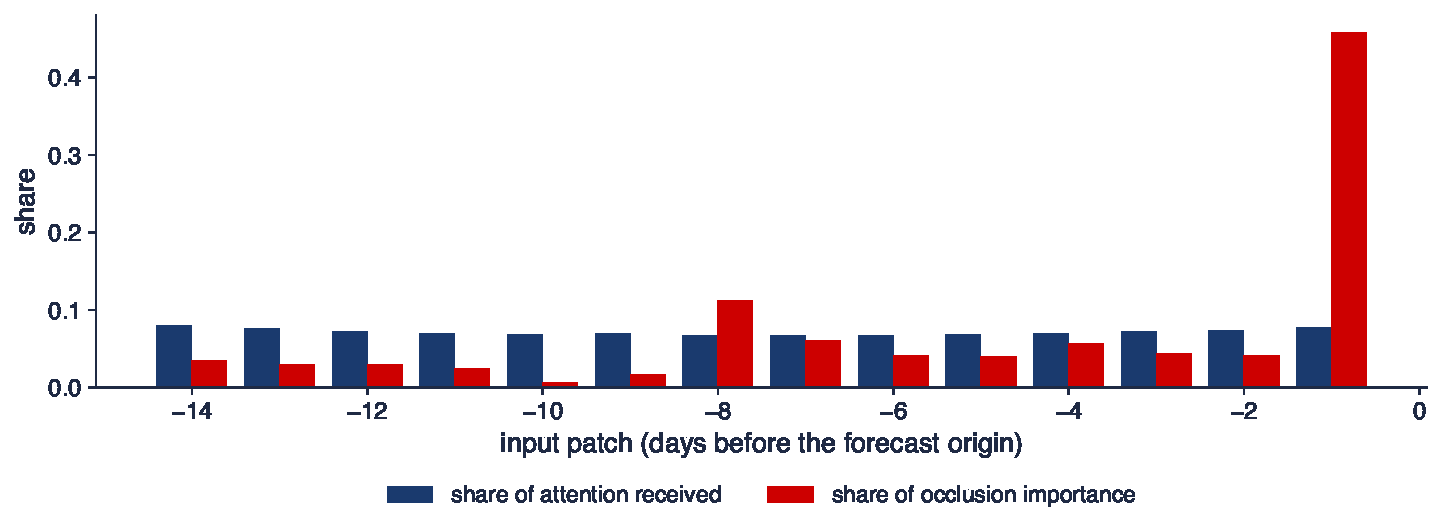
\includegraphics[width=0.97\textwidth,height=0.46\textheight,keepaspectratio]{ats_ch12_attention.pdf}
\end{center}
\vspace{-0.25cm}
\begin{itemize}
    \item Ponderea atenției primite de fiecare dintre cele 14 segmente zilnice față de ponderea importanței prin ocluzie
\end{itemize}
\quantlet{ATS\_ch12\_interpretation}{\qlurl{ATS_ch12_interpretation}}
\end{frame}

\begin{frame}{Interpretarea atenției și ocluziei}
\itemsize{\small}
\begin{itemize}
    \item Ultima zi poartă 46\% din importanța prin ocluzie, dar primește doar 8\% din atenție
    \item Cea mai mare atenție merge la segmentul de acum 14 zile; cel mai important segment este cel de acum 1 zi; corelația Spearman \ensuremath{-}0{,}09
    \item Capul care aplatizează citește direct stările tokenilor: ce contează poate ocoli complet ponderile atenției
    \item Raportați hărțile de atenție drept ceea ce sînt, un tipar de amestecare; pentru importanță folosiți ocluzia, Shapley sau gradienții, cu o verificare de control
\end{itemize}
\end{frame}

\begin{frame}{Comparația riguroasă}
\itemsize{\small}
\begin{itemize}
    \item Întîi repere puternice: naiv sezonier, ETS/Theta, HAR, un ARX expert; Lago et al.\ au construit un reper deschis pentru că modelele publicate de prețuri ale electricității erau rar comparate cu ele \refLMDW
    \item Capcanele inventariate de \refHAB: reutilizarea setului de test, scurgeri prin scalare și variabile, erori mediate pe serii de scări diferite, fără teste de semnificație, buget de reglare neraportat
    \item Teste (\atschlink{https://danpele.github.io/Advanced-Time-Series/RO/Cursuri/capitol1_evaluarea_prognozelor.pdf}{Capitolul 1}): DM pentru două modele, MCS \refHLN\ pentru mai multe, reality check \refWhi\ și SPA \refHan\ cînd cel mai bun dintre multe a fost ales pe aceleași date
    \item Raportați seed-urile, hardware-ul, timpul de antrenare, fiecare arhitectură încercată; preînregistrați schema (\atschlink{https://danpele.github.io/Advanced-Time-Series/RO/Cursuri/capitol0_recapitulare_inferenta.pdf}{Capitolul 0})
\end{itemize}
\end{frame}

\begin{frame}{Seed-uri și data snooping}
\itemsize{\footnotesize}
\begin{center}
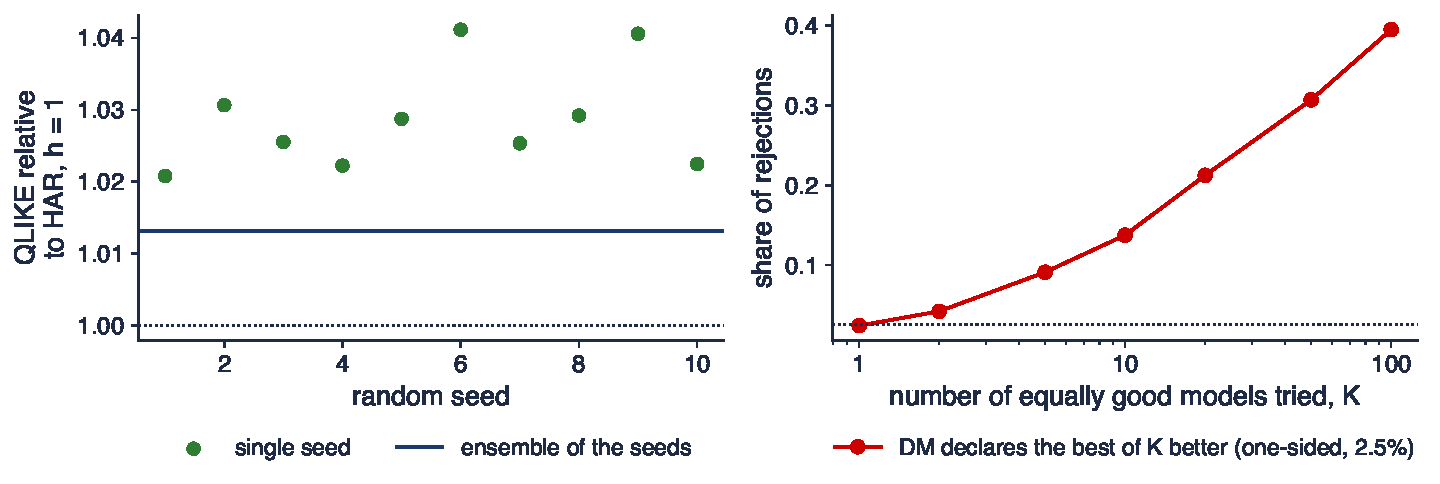
\includegraphics[width=0.97\textwidth,height=0.46\textheight,keepaspectratio]{ats_ch12_snooping.pdf}
\end{center}
\vspace{-0.25cm}
\begin{itemize}
    \item Stînga: MLP față de HAR pentru RV S\&P 500, $h = 1$, cu 10 seed-uri și ansamblul lor; dreapta: simulare, $K$ modele la fel de bune, 2500 de zile de test, corelație 0,5
\end{itemize}
\quantlet{ATS\_ch12\_interpretation}{\qlurl{ATS_ch12_interpretation}}
\end{frame}

\begin{frame}{Interpretarea seed-urilor și a data snooping}
\itemsize{\small}
\begin{itemize}
    \item Doar seed-urile mută raportul QLIKE între 1{,}019 și 1{,}041 (mediana 1{,}027); ansamblul seed-urilor ajunge la 1{,}013, mai bun decît orice seed individual
    \item Alegerea celui mai bun dintre $K$ modele la fel de bune pe setul de test: testul DM îl declară mai bun (unilateral, nivel nominal 2,5\%) în 2\% din cazuri pentru $K = 1$, 14\% pentru $K = 10$, 40\% pentru $K = 100$
    \item Căutările de hiperparametri, seed-urile și arhitecturile sînt toate $K$: numărați-le și testați cîștigătorul cu SPA sau MCS pe date nefolosite pentru alegere
    \item Ansamblurile sînt remediul ieftin pentru varianța seed-urilor; preînregistrarea este remediul pentru data snooping
\end{itemize}
\end{frame}

\begin{frame}{Recapitulare: interpretare și comparații riguroase}
\itemsize{\small}
\begin{itemize}
    \item Valorile Shapley au axiome; cu variabile întîrziate folosiți grupuri și amintiți-vă că ele descriu modelul
    \item Ponderile atenției nu sînt importanță: pe Transformer-ul nostru ele indică în direcția opusă
    \item Repere puternice, DM/MCS/SPA, toate seed-urile și toate încercările raportate: altfel orice model poate fi făcut să cîștige
\end{itemize}
\end{frame}


%=============================================================================
\section{AI în descoperirea științifică}
%=============================================================================

\begin{frame}{O întrebare deschisă}
\itemsize{\small}
\begin{itemize}
    \item Prognozează modelele de machine learning și deep learning volatilitatea realizată mai bine decît HAR, pe mai multe piețe și orizonturi, atunci cînd comparația este preînregistrată?
    \begin{itemize}
        \item formal: $H_0$: $\E[\mathrm{QLIKE}_{\mathrm{ML}} - \mathrm{QLIKE}_{\mathrm{HAR}}] \ge 0$ în fiecare celulă; o celulă susține ML doar dacă DM respinge la 5\% și MCS exclude HAR
        \item infirmată dacă mai puțin de o cincime din celule susțin ML
    \end{itemize}
    \item Miza: sistemele de risc (VaR, marje, acoperirea opțiunilor) se bazează pe prognoze de volatilitate; un cîștig ML aparent devine un risc de model
    \begin{itemize}
        \item literatura de pornire: \refCor, \refBuc, \refCSV, \refHAB
    \end{itemize}
\end{itemize}
\end{frame}

\begin{frame}{Bucla de cercetare cu un asistent AI}
\itemsize{\footnotesize}
\begin{itemize}
    \item Un asistent AI (un LLM precum Claude, ChatGPT, Gemini sau Copilot) accelerează fiecare etapă; Semantic Scholar și Elicit ajută la literatură
    \begin{itemize}
        \item \textbf{literatura}: \aiprompt{Listează articole recenzate din 2019 încoace care compară rețele neuronale sau boosting cu HAR pentru volatilitatea realizată în afara eșantionului; dă DOI-urile și testul folosit.} Apoi verificați fiecare DOI pe Crossref
        \item \textbf{schema}: \aiprompt{Scrie o preînregistrare: active, orizonturi, ferestre, calendarul reestimării, pierderea, testele, seed-urile, ce înseamnă un cîștig.}
        \item \textbf{cod și replicare}: reproduceți întîi QLIKE HAR pentru S\&P 500 (0{,}253 la $h = 1$ aici), apoi adăugați algoritmii pe rînd
        \item \textbf{critica}: \aiprompt{Joacă rolul unui recenzent ostil: enumeră fiecare sursă de scurgere de informație, data snooping și reglare inechitabilă din această comparație.}
    \end{itemize}
    \item Raportul: ce s-a cerut, ce s-a păstrat, ce s-a respins (AI\_USE.md, AI\_ERRORS.md)
\end{itemize}
\end{frame}

\begin{frame}{Verificări necesare}
\itemsize{\small}
\begin{itemize}
    \item Fiecare referință există și spune ce se afirmă (DOI-ul funcționează, titlul coincide, rezultatul se află în lucrare)
    \item Nicio informație din viitor: scalarea, construcția variabilelor și reglarea folosesc doar date dinaintea fiecărei origini; purjare în jurul țintelor la $h$ pași
    \item Reperul este reglat la fel de atent ca algoritmul și reestimat după același calendar
    \item Seed-urile, arhitecturile și hiperparametrii încercați sînt toți raportați; cîștigătorul este testat cu MCS sau SPA
    \item O afirmație AI de tipul „LSTM captează memoria lungă, deci este mai bun decît HAR” se verifică pe cifre, nu se acceptă
\end{itemize}
\end{frame}

\begin{frame}{Mini studiu de caz: algoritmii față de HAR pe mai multe piețe}
\itemsize{\footnotesize}
\begin{center}
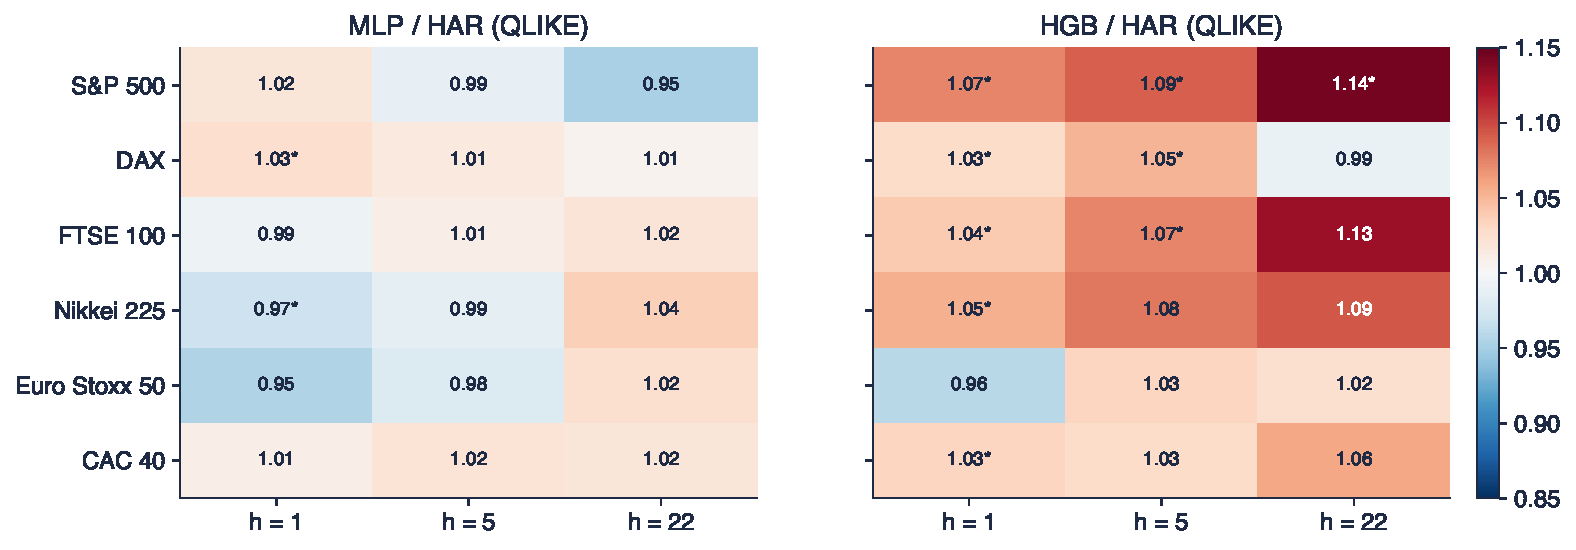
\includegraphics[width=0.97\textwidth,height=0.44\textheight,keepaspectratio]{ats_ch12_ai_case.pdf}
\end{center}
\vspace{-0.25cm}
\begin{itemize}
    \item 36 de celule: șase indici $\times$ trei orizonturi $\times$ doi algoritmi (MLP, boosting), schema cu fereastră extinsă din secțiunea 4; raportul QLIKE față de HAR, o stea unde DM respinge la 5\%
    \item Rapoarte între 0{,}95 și 1{,}14, mediana 1{,}024 (MLP 1{,}009, boosting 1{,}052); 9 celule sub 1, 1 semnificativ mai bune, 10 semnificativ mai slabe: ipoteza este infirmată pentru acești algoritmi
\end{itemize}
\quantlet{ATS\_ch12\_ai\_case}{\qlurl{ATS_ch12_ai_case}}
\end{frame}

\begin{frame}{Idee de proiect}
\itemsize{\small}
\begin{itemize}
    \item \textbf{Deep learning față de HAR pentru volatilitatea din Europa Centrală și de Est}: întîi replicare, apoi extindere
    \begin{itemize}
        \item replicați: HAR \refCor\ și comparația neuronală din \refBuc\ pe indicii Oxford-Man, cu schema din secțiunea 4
        \item extindeți: RV din date intraday pentru BET, WIG20 și EUR/RON; modele globale pe mai multe piețe; predictori exogeni (VIX, știri macro) ca în \refCSV
        \item preînregistrați: piețele, orizonturile, ferestrele, fiecare algoritm și bugetul lui de reglare, QLIKE, DM, MCS, seed-urile
    \end{itemize}
    \item Livrabilele urmează regulile cursului: repository, raport, AI\_USE.md, AI\_ERRORS.md, susținere orală
\end{itemize}
\end{frame}


%=============================================================================
\section{Încheiere}
%=============================================================================

\begin{frame}{Idei de reținut}
\itemsize{\small}
\begin{itemize}
    \item Validarea trebuie să respecte dependența: K subeșantioane doar pentru autoregresii bine specificate; altfel blocuri, purjare și o perioadă finală de test
    \item Modelele globale reunesc seriile și își permit memorie; selecția în dimensiune mare pe eșantioane macro scurte este instabilă
    \item Arborii și rețelele depășesc rar, singure, reperele puternice și structurate (ARX expert, HAR); ajută în combinații și în paneluri mari
    \item Detaliile de arhitectură contează: porți de uitare deschise, segmente în loc de tokeni punctuali, antrenare globală
    \item Atenția nu este explicație; seed-urile și căutările sînt testare multiplă ascunsă
\end{itemize}
\end{frame}

\begin{frame}{Autoevaluare}
\itemsize{\small}
\begin{columns}[T]
\begin{column}{0.58\textwidth}
\begin{block}{Întrebări}
\begin{itemize}
    \item De ce este validă validarea cu K subeșantioane aleatoare pentru un AR(3) estimat pe date AR(3), dar nu pentru ținte de 22 de zile?
    \item Ce condiție elimină lasso-ul adaptiv și cum?
    \item De ce adăugarea de arbori nu reduce varianța unei păduri sub $\rho\sigma^2$?
    \item Care este cîmpul receptiv al unui TCN cu $k = 3$ și cinci niveluri?
    \item De ce poate un Transformer pe segmente să fie mai bun decît DLinear, iar unul cu tokeni punctuali nu?
\end{itemize}
\end{block}
\end{column}
\begin{column}{0.38\textwidth}
\begin{block}{Urmează: \atschlink{https://danpele.github.io/Advanced-Time-Series/RO/Cursuri/capitol13_foundation_models_conformal.pdf}{Capitolul 13}}
\begin{itemize}
    \item Foundation models și predicție conformală
    \item modele preantrenate folosite zero-shot și intervale fără ipoteze de distribuție pentru orice model, inclusiv cele din acest capitol
\end{itemize}
\end{block}
\end{column}
\end{columns}
\end{frame}


%=============================================================================
\section{Anexă}
%=============================================================================

\begin{frame}{Anexă: deplasarea validării cu K subeșantioane sub erori autocorelate}
\itemsize{\small}
\begin{itemize}
    \item Model liniar $y = X\beta + \varepsilon$; omitem rîndul $i$: $e_{(i)} = e_i/(1 - h_{ii})$, $h_{ii}$ efectul de pîrghie
    \item $\E\,e_{(i)}^2 \approx \sigma^2(1 + h_{ii}) - 2\sum_{j\ne i}\frac{H_{ij}}{1 - h_{ii}}\Cov(\varepsilon_i, \varepsilon_j)$, la ordinul întîi
    \item Erori necorelate: al doilea termen dispare, iar LOOCV estimează MSE în afara eșantionului $\sigma^2(1 + h)$: cazul Bergmeir--Hyndman--Koo
    \item Corelație pozitivă între eroarea omisă și erorile de antrenare vecine ($H_{ij} > 0$ pentru vecinii cu laguri asemănătoare): estimația este prea mică; purjarea anulează termenii vecini
\end{itemize}
\end{frame}

\begin{frame}{Anexă: pragul moale și elastic net}
\itemsize{\small}
\begin{itemize}
    \item Cu $X'X = nI$, funcția obiectiv se separă: $\frac12(\beta_j - z_j)^2 + \lambda|\beta_j|$ pentru fiecare $j$, $z_j = x_j'y/n$
    \item Subgradientul: $0 \in \beta_j - z_j + \lambda\,\partial|\beta_j|$; dacă $|z_j| \le \lambda$, $\beta_j = 0$; altfel $\beta_j = z_j - \lambda\,\mathrm{sign}(z_j)$
    \item Elastic net: $\frac12(\beta_j - z_j)^2 + \lambda\alpha|\beta_j| + \frac{\lambda(1 - \alpha)}2\beta_j^2$ dă $\beta_j = S(z_j, \lambda\alpha)/(1 + \lambda(1 - \alpha))$
    \item Lasso adaptiv: pragul $\lambda w_j = \lambda/|\tilde\beta_j|^\gamma$, mic pentru $|\tilde\beta_j|$ mare: deplasarea coeficienților mari dispare, de unde proprietatea de oracol
\end{itemize}
\end{frame}


%=============================================================================
\section{Bibliografie}
%=============================================================================

\begin{frame}{Bibliografie (1/6)}
\itemsize{\tiny}
\begin{itemize}
    \item Bai, S., Kolter, J. Z., \& Koltun, V. (2018). An empirical evaluation of generic convolutional and recurrent networks for sequence modeling. arXiv:1803.01271. \href{https://arxiv.org/abs/1803.01271}{arxiv.org}
    \item Basu, S., \& Michailidis, G. (2015). Regularized estimation in sparse high-dimensional time series models. \textit{The Annals of Statistics}, 43(4), 1535--1567. \href{https://doi.org/10.1214/15-AOS1315}{doi:10.1214/15-AOS1315}
    \item Belloni, A., Chernozhukov, V., \& Hansen, C. (2014). Inference on treatment effects after selection among high-dimensional controls. \textit{The Review of Economic Studies}, 81(2), 608--650. \href{https://doi.org/10.1093/restud/rdt044}{doi:10.1093/restud/rdt044}
    \item Bengio, Y., Simard, P., \& Frasconi, P. (1994). Learning long-term dependencies with gradient descent is difficult. \textit{IEEE Transactions on Neural Networks}, 5(2), 157--166. \href{https://doi.org/10.1109/72.279181}{doi:10.1109/72.279181}
    \item Benidis, K., Rangapuram, S. S., Flunkert, V., Wang, Y., et al.\ (2022). Deep learning for time series forecasting: Tutorial and literature survey. \textit{ACM Computing Surveys}, 55(6), 1--36. \href{https://doi.org/10.1145/3533382}{doi:10.1145/3533382}
    \item Bergmeir, C., \& Benítez, J. M. (2012). On the use of cross-validation for time series predictor evaluation. \textit{Information Sciences}, 191, 192--213. \href{https://doi.org/10.1016/j.ins.2011.12.028}{doi:10.1016/j.ins.2011.12.028}
    \item Bergmeir, C., Hyndman, R. J., \& Koo, B. (2018). A note on the validity of cross-validation for evaluating autoregressive time series prediction. \textit{Computational Statistics \& Data Analysis}, 120, 70--83. \href{https://doi.org/10.1016/j.csda.2017.11.003}{doi:10.1016/j.csda.2017.11.003}
    \item Berk, R., Brown, L., Buja, A., Zhang, K., \& Zhao, L. (2013). Valid post-selection inference. \textit{The Annals of Statistics}, 41(2), 802--837. \href{https://doi.org/10.1214/12-AOS1077}{doi:10.1214/12-AOS1077}
    \item Breiman, L. (1996). Bagging predictors. \textit{Machine Learning}, 24(2), 123--140. \href{https://doi.org/10.1007/BF00058655}{doi:10.1007/BF00058655}
    \item Breiman, L. (2001). Random forests. \textit{Machine Learning}, 45(1), 5--32. \href{https://doi.org/10.1023/A:1010933404324}{doi:10.1023/A:1010933404324}
    \item Bucci, A. (2020). Realized volatility forecasting with neural networks. \textit{Journal of Financial Econometrics}, 18(3), 502--531. \href{https://doi.org/10.1093/jjfinec/nbaa008}{doi:10.1093/jjfinec/nbaa008}
    \item Burman, P., Chow, E., \& Nolan, D. (1994). A cross-validatory method for dependent data. \textit{Biometrika}, 81(2), 351--358. \href{https://doi.org/10.1093/biomet/81.2.351}{doi:10.1093/biomet/81.2.351}
    \item Challu, C., Olivares, K. G., Oreshkin, B. N., Garza Ramirez, F., Mergenthaler Canseco, M., \& Dubrawski, A. (2023). NHITS: Neural hierarchical interpolation for time series forecasting. \textit{Proceedings of the AAAI Conference on Artificial Intelligence}, 37(6), 6989--6997. \href{https://doi.org/10.1609/aaai.v37i6.25854}{doi:10.1609/aaai.v37i6.25854}
    \item Chen, T., \& Guestrin, C. (2016). XGBoost: A scalable tree boosting system. \textit{Proceedings of the 22nd ACM SIGKDD International Conference on Knowledge Discovery and Data Mining}, 785--794. \href{https://doi.org/10.1145/2939672.2939785}{doi:10.1145/2939672.2939785}
\end{itemize}
\end{frame}

\begin{frame}{Bibliografie (2/6)}
\itemsize{\tiny}
\begin{itemize}
    \item Cho, K., van Merriënboer, B., Gulcehre, C., Bahdanau, D., Bougares, F., Schwenk, H., \& Bengio, Y. (2014). Learning phrase representations using RNN encoder--decoder for statistical machine translation. \textit{Proceedings of EMNLP 2014}, 1724--1734. \href{https://doi.org/10.3115/v1/D14-1179}{doi:10.3115/v1/D14-1179}
    \item Christensen, K., Siggaard, M., \& Veliyev, B. (2023). A machine learning approach to volatility forecasting. \textit{Journal of Financial Econometrics}, 21(5), 1680--1727. \href{https://doi.org/10.1093/jjfinec/nbac020}{doi:10.1093/jjfinec/nbac020}
    \item Corsi, F. (2009). A simple approximate long-memory model of realized volatility. \textit{Journal of Financial Econometrics}, 7(2), 174--196. \href{https://doi.org/10.1093/jjfinec/nbp001}{doi:10.1093/jjfinec/nbp001}
    \item Diebold, F. X., \& Mariano, R. S. (1995). Comparing predictive accuracy. \textit{Journal of Business \& Economic Statistics}, 13(3), 253--263. \href{https://doi.org/10.1080/07350015.1995.10524599}{doi:10.1080/07350015.1995.10524599}
    \item Friedman, J. H. (2001). Greedy function approximation: A gradient boosting machine. \textit{The Annals of Statistics}, 29(5), 1189--1232. \href{https://doi.org/10.1214/aos/1013203451}{doi:10.1214/aos/1013203451}
    \item Gers, F. A., Schmidhuber, J., \& Cummins, F. (2000). Learning to forget: Continual prediction with LSTM. \textit{Neural Computation}, 12(10), 2451--2471. \href{https://doi.org/10.1162/089976600300015015}{doi:10.1162/089976600300015015}
    \item Gneiting, T., \& Raftery, A. E. (2007). Strictly proper scoring rules, prediction, and estimation. \textit{Journal of the American Statistical Association}, 102(477), 359--378. \href{https://doi.org/10.1198/016214506000001437}{doi:10.1198/016214506000001437}
    \item Goulet Coulombe, P., Leroux, M., Stevanovic, D., \& Surprenant, S. (2022). How is machine learning useful for macroeconomic forecasting? \textit{Journal of Applied Econometrics}, 37(5), 920--964. \href{https://doi.org/10.1002/jae.2910}{doi:10.1002/jae.2910}
    \item Gu, S., Kelly, B., \& Xiu, D. (2020). Empirical asset pricing via machine learning. \textit{The Review of Financial Studies}, 33(5), 2223--2273. \href{https://doi.org/10.1093/rfs/hhaa009}{doi:10.1093/rfs/hhaa009}
    \item Hansen, P. R. (2005). A test for superior predictive ability. \textit{Journal of Business \& Economic Statistics}, 23(4), 365--380. \href{https://doi.org/10.1198/073500105000000063}{doi:10.1198/073500105000000063}
    \item Hansen, P. R., Lunde, A., \& Nason, J. M. (2011). The model confidence set. \textit{Econometrica}, 79(2), 453--497. \href{https://doi.org/10.3982/ECTA5771}{doi:10.3982/ECTA5771}
    \item Heber, G., Lunde, A., Shephard, N., \& Sheppard, K. K. (2009). Oxford-Man Institute\'s realized library, version 0.3. Oxford-Man Institute, University of Oxford. \href{https://web.archive.org/web/20220301022212/https://realized.oxford-man.ox.ac.uk/}{web.archive.org}
    \item Hewamalage, H., Ackermann, K., \& Bergmeir, C. (2023). Forecast evaluation for data scientists: Common pitfalls and best practices. \textit{Data Mining and Knowledge Discovery}, 37(2), 788--832. \href{https://doi.org/10.1007/s10618-022-00894-5}{doi:10.1007/s10618-022-00894-5}
    \item Hewamalage, H., Bergmeir, C., \& Bandara, K. (2021). Recurrent neural networks for time series forecasting: Current status and future directions. \textit{International Journal of Forecasting}, 37(1), 388--427. \href{https://doi.org/10.1016/j.ijforecast.2020.06.008}{doi:10.1016/j.ijforecast.2020.06.008}
\end{itemize}
\end{frame}

\begin{frame}{Bibliografie (3/6)}
\itemsize{\tiny}
\begin{itemize}
    \item Hochreiter, S., \& Schmidhuber, J. (1997). Long short-term memory. \textit{Neural Computation}, 9(8), 1735--1780. \href{https://doi.org/10.1162/neco.1997.9.8.1735}{doi:10.1162/neco.1997.9.8.1735}
    \item Hyndman, R. J., \& Koehler, A. B. (2006). Another look at measures of forecast accuracy. \textit{International Journal of Forecasting}, 22(4), 679--688. \href{https://doi.org/10.1016/j.ijforecast.2006.03.001}{doi:10.1016/j.ijforecast.2006.03.001}
    \item Jain, S., \& Wallace, B. C. (2019). Attention is not explanation. \textit{Proceedings of NAACL-HLT 2019}, 3543--3556. \href{https://doi.org/10.18653/v1/N19-1357}{doi:10.18653/v1/N19-1357}
    \item Jozefowicz, R., Zaremba, W., \& Sutskever, I. (2015). An empirical exploration of recurrent network architectures. \textit{Proceedings of the 32nd International Conference on Machine Learning}, PMLR 37, 2342--2350. \href{https://proceedings.mlr.press/v37/jozefowicz15.html}{proceedings.mlr.press}
    \item Ke, G., Meng, Q., Finley, T., Wang, T., Chen, W., Ma, W., Ye, Q., \& Liu, T.-Y. (2017). LightGBM: A highly efficient gradient boosting decision tree. \textit{Advances in Neural Information Processing Systems}, 30. \href{https://proceedings.neurips.cc/paper/2017/hash/6449f44a102fde848669bdd9eb6b76fa-Abstract.html}{proceedings.neurips.cc}
    \item Kingma, D. P., \& Ba, J. (2015). Adam: A method for stochastic optimization. \textit{International Conference on Learning Representations}. arXiv:1412.6980. \href{https://arxiv.org/abs/1412.6980}{arxiv.org}
    \item Lago, J., Marcjasz, G., De Schutter, B., \& Weron, R. (2021). Forecasting day-ahead electricity prices: A review of state-of-the-art algorithms, best practices and an open-access benchmark. \textit{Applied Energy}, 293, 116983. \href{https://doi.org/10.1016/j.apenergy.2021.116983}{doi:10.1016/j.apenergy.2021.116983}
    \item Lee, J. D., Sun, D. L., Sun, Y., \& Taylor, J. E. (2016). Exact post-selection inference, with application to the lasso. \textit{The Annals of Statistics}, 44(3), 907--927. \href{https://doi.org/10.1214/15-AOS1371}{doi:10.1214/15-AOS1371}
    \item Lim, B., Arık, S. Ö., Loeff, N., \& Pfister, T. (2021). Temporal fusion transformers for interpretable multi-horizon time series forecasting. \textit{International Journal of Forecasting}, 37(4), 1748--1764. \href{https://doi.org/10.1016/j.ijforecast.2021.03.012}{doi:10.1016/j.ijforecast.2021.03.012}
    \item Lundberg, S. M., \& Lee, S.-I. (2017). A unified approach to interpreting model predictions. \textit{Advances in Neural Information Processing Systems}, 30. \href{https://proceedings.neurips.cc/paper/2017/hash/8a20a8621978632d76c43dfd28b67767-Abstract.html}{proceedings.neurips.cc}
    \item Makridakis, S., Spiliotis, E., \& Assimakopoulos, V. (2022). M5 accuracy competition: Results, findings, and conclusions. \textit{International Journal of Forecasting}, 38(4), 1346--1364. \href{https://doi.org/10.1016/j.ijforecast.2021.11.013}{doi:10.1016/j.ijforecast.2021.11.013}
    \item Makridakis, S., Spiliotis, E., \& Assimakopoulos, V. (2018). Statistical and machine learning forecasting methods: Concerns and ways forward. \textit{PLOS ONE}, 13(3), e0194889. \href{https://doi.org/10.1371/journal.pone.0194889}{doi:10.1371/journal.pone.0194889}
    \item Makridakis, S., Spiliotis, E., \& Assimakopoulos, V. (2020). The M4 Competition: 100,000 time series and 61 forecasting methods. \textit{International Journal of Forecasting}, 36(1), 54--74. \href{https://doi.org/10.1016/j.ijforecast.2019.04.014}{doi:10.1016/j.ijforecast.2019.04.014}
    \item Medeiros, M. C., \& Mendes, E. F. (2016). $\ell_1$-regularization of high-dimensional time-series models with non-Gaussian and heteroskedastic errors. \textit{Journal of Econometrics}, 191(1), 255--271. \href{https://doi.org/10.1016/j.jeconom.2015.10.011}{doi:10.1016/j.jeconom.2015.10.011}
\end{itemize}
\end{frame}

\begin{frame}{Bibliografie (4/6)}
\itemsize{\tiny}
\begin{itemize}
    \item Medeiros, M. C., Vasconcelos, G. F. R., Veiga, Á., \& Zilberman, E. (2021). Forecasting inflation in a data-rich environment: The benefits of machine learning methods. \textit{Journal of Business \& Economic Statistics}, 39(1), 98--119. \href{https://doi.org/10.1080/07350015.2019.1637745}{doi:10.1080/07350015.2019.1637745}
    \item Meinshausen, N. (2006). Quantile regression forests. \textit{Journal of Machine Learning Research}, 7, 983--999. \href{https://jmlr.org/papers/v7/meinshausen06a.html}{jmlr.org}
    \item Mohri, M., \& Rostamizadeh, A. (2010). Stability bounds for stationary $\varphi$-mixing and $\beta$-mixing processes. \textit{Journal of Machine Learning Research}, 11, 789--814. \href{https://jmlr.org/papers/v11/mohri10a.html}{jmlr.org}
    \item Montero-Manso, P., \& Hyndman, R. J. (2021). Principles and algorithms for forecasting groups of time series: Locality and globality. \textit{International Journal of Forecasting}, 37(4), 1632--1653. \href{https://doi.org/10.1016/j.ijforecast.2021.03.004}{doi:10.1016/j.ijforecast.2021.03.004}
    \item Nie, Y., Nguyen, N. H., Sinthong, P., \& Kalagnanam, J. (2023). A time series is worth 64 words: Long-term forecasting with Transformers. \textit{International Conference on Learning Representations}. arXiv:2211.14730. \href{https://arxiv.org/abs/2211.14730}{arxiv.org}
    \item Oreshkin, B. N., Carpov, D., Chapados, N., \& Bengio, Y. (2020). N-BEATS: Neural basis expansion analysis for interpretable time series forecasting. \textit{International Conference on Learning Representations}. arXiv:1905.10437. \href{https://arxiv.org/abs/1905.10437}{arxiv.org}
    \item Pascanu, R., Mikolov, T., \& Bengio, Y. (2013). On the difficulty of training recurrent neural networks. \textit{Proceedings of the 30th International Conference on Machine Learning}, PMLR 28(3), 1310--1318. \href{https://proceedings.mlr.press/v28/pascanu13.html}{proceedings.mlr.press}
    \item Patton, A. J. (2011). Volatility forecast comparison using imperfect volatility proxies. \textit{Journal of Econometrics}, 160(1), 246--256. \href{https://doi.org/10.1016/j.jeconom.2010.03.034}{doi:10.1016/j.jeconom.2010.03.034}
    \item Petropoulos, F., Apiletti, D., Assimakopoulos, V., Babai, M. Z., et al.\ (2022). Forecasting: Theory and practice. \textit{International Journal of Forecasting}, 38(3), 705--871. \href{https://doi.org/10.1016/j.ijforecast.2021.11.001}{doi:10.1016/j.ijforecast.2021.11.001}
    \item Racine, J. (2000). Consistent cross-validatory model-selection for dependent data: hv-block cross-validation. \textit{Journal of Econometrics}, 99(1), 39--61. \href{https://doi.org/10.1016/S0304-4076(00)00030-0}{doi:10.1016/S0304-4076(00)00030-0}
    \item Rumelhart, D. E., Hinton, G. E., \& Williams, R. J. (1986). Learning representations by back-propagating errors. \textit{Nature}, 323(6088), 533--536. \href{https://doi.org/10.1038/323533a0}{doi:10.1038/323533a0}
    \item Salinas, D., Flunkert, V., Gasthaus, J., \& Januschowski, T. (2020). DeepAR: Probabilistic forecasting with autoregressive recurrent networks. \textit{International Journal of Forecasting}, 36(3), 1181--1191. \href{https://doi.org/10.1016/j.ijforecast.2019.07.001}{doi:10.1016/j.ijforecast.2019.07.001}
    \item Scornet, E., Biau, G., \& Vert, J.-P. (2015). Consistency of random forests. \textit{The Annals of Statistics}, 43(4), 1716--1741. \href{https://doi.org/10.1214/15-AOS1321}{doi:10.1214/15-AOS1321}
    \item Shapley, L. S. (1953). A value for $n$-person games. In H. W. Kuhn \& A. W. Tucker (Eds.), \textit{Contributions to the Theory of Games II}, 307--318. Princeton University Press. \href{https://doi.org/10.1515/9781400881970-018}{doi:10.1515/9781400881970-018}
\end{itemize}
\end{frame}

\begin{frame}{Bibliografie (5/6)}
\itemsize{\tiny}
\begin{itemize}
    \item Smyl, S. (2020). A hybrid method of exponential smoothing and recurrent neural networks for time series forecasting. \textit{International Journal of Forecasting}, 36(1), 75--85. \href{https://doi.org/10.1016/j.ijforecast.2019.03.017}{doi:10.1016/j.ijforecast.2019.03.017}
    \item Sutskever, I., Vinyals, O., \& Le, Q. V. (2014). Sequence to sequence learning with neural networks. \textit{Advances in Neural Information Processing Systems}, 27. arXiv:1409.3215. \href{https://arxiv.org/abs/1409.3215}{arxiv.org}
    \item Tibshirani, R. (1996). Regression shrinkage and selection via the lasso. \textit{Journal of the Royal Statistical Society: Series B}, 58(1), 267--288. \href{https://doi.org/10.1111/j.2517-6161.1996.tb02080.x}{doi:10.1111/j.2517-6161.1996.tb02080.x}
    \item van den Oord, A., Dieleman, S., Zen, H., Simonyan, K., Vinyals, O., Graves, A., Kalchbrenner, N., Senior, A., \& Kavukcuoglu, K. (2016). WaveNet: A generative model for raw audio. arXiv:1609.03499. \href{https://arxiv.org/abs/1609.03499}{arxiv.org}
    \item Vaswani, A., Shazeer, N., Parmar, N., Uszkoreit, J., Jones, L., Gomez, A. N., Kaiser, Ł., \& Polosukhin, I. (2017). Attention is all you need. \textit{Advances in Neural Information Processing Systems}, 30. \href{https://proceedings.neurips.cc/paper/2017/hash/3f5ee243547dee91fbd053c1c4a845aa-Abstract.html}{proceedings.neurips.cc}
    \item Wager, S., \& Athey, S. (2018). Estimation and inference of heterogeneous treatment effects using random forests. \textit{Journal of the American Statistical Association}, 113(523), 1228--1242. \href{https://doi.org/10.1080/01621459.2017.1319839}{doi:10.1080/01621459.2017.1319839}
    \item White, H. (2000). A reality check for data snooping. \textit{Econometrica}, 68(5), 1097--1126. \href{https://doi.org/10.1111/1468-0262.00152}{doi:10.1111/1468-0262.00152}
    \item Wiegreffe, S., \& Pinter, Y. (2019). Attention is not not explanation. \textit{Proceedings of EMNLP-IJCNLP 2019}, 11--20. \href{https://doi.org/10.18653/v1/D19-1002}{doi:10.18653/v1/D19-1002}
    \item Wu, H., Xu, J., Wang, J., \& Long, M. (2021). Autoformer: Decomposition transformers with auto-correlation for long-term series forecasting. \textit{Advances in Neural Information Processing Systems}, 34. \href{https://proceedings.neurips.cc/paper/2021/hash/bcc0d400288793e8bdcd7c19a8ac0c2b-Abstract.html}{proceedings.neurips.cc}
    \item Yu, B. (1994). Rates of convergence for empirical processes of stationary mixing sequences. \textit{The Annals of Probability}, 22(1), 94--116. \href{https://doi.org/10.1214/aop/1176988849}{doi:10.1214/aop/1176988849}
    \item Zeng, A., Chen, M., Zhang, L., \& Xu, Q. (2023). Are transformers effective for time series forecasting? \textit{Proceedings of the AAAI Conference on Artificial Intelligence}, 37(9), 11121--11128. \href{https://doi.org/10.1609/aaai.v37i9.26317}{doi:10.1609/aaai.v37i9.26317}
    \item Zhao, P., \& Yu, B. (2006). On model selection consistency of lasso. \textit{Journal of Machine Learning Research}, 7, 2541--2563. \href{https://jmlr.org/papers/v7/zhao06a.html}{jmlr.org}
    \item Zhou, H., Zhang, S., Peng, J., Zhang, S., Li, J., Xiong, H., \& Zhang, W. (2021). Informer: Beyond efficient transformer for long sequence time-series forecasting. \textit{Proceedings of the AAAI Conference on Artificial Intelligence}, 35(12), 11106--11115. \href{https://doi.org/10.1609/aaai.v35i12.17325}{doi:10.1609/aaai.v35i12.17325}
    \item Ziel, F., \& Weron, R. (2018). Day-ahead electricity price forecasting with high-dimensional structures: Univariate vs. multivariate modeling frameworks. \textit{Energy Economics}, 70, 396--420. \href{https://doi.org/10.1016/j.eneco.2017.12.016}{doi:10.1016/j.eneco.2017.12.016}
\end{itemize}
\end{frame}

\begin{frame}{Bibliografie (6/6)}
\itemsize{\tiny}
\begin{itemize}
    \item Zou, H., \& Hastie, T. (2005). Regularization and variable selection via the elastic net. \textit{Journal of the Royal Statistical Society: Series B}, 67(2), 301--320. \href{https://doi.org/10.1111/j.1467-9868.2005.00503.x}{doi:10.1111/j.1467-9868.2005.00503.x}
    \item Zou, H. (2006). The adaptive lasso and its oracle properties. \textit{Journal of the American Statistical Association}, 101(476), 1418--1429. \href{https://doi.org/10.1198/016214506000000735}{doi:10.1198/016214506000000735}
\end{itemize}
\end{frame}

\end{document}
